\documentclass[]{article}
\usepackage{lmodern}
\usepackage{amssymb,amsmath}
\usepackage{ifxetex,ifluatex}
\usepackage{fixltx2e} % provides \textsubscript
\ifnum 0\ifxetex 1\fi\ifluatex 1\fi=0 % if pdftex
  \usepackage[T1]{fontenc}
  \usepackage[utf8]{inputenc}
\else % if luatex or xelatex
  \ifxetex
    \usepackage{mathspec}
  \else
    \usepackage{fontspec}
  \fi
  \defaultfontfeatures{Ligatures=TeX,Scale=MatchLowercase}
\fi
% use upquote if available, for straight quotes in verbatim environments
\IfFileExists{upquote.sty}{\usepackage{upquote}}{}
% use microtype if available
\IfFileExists{microtype.sty}{%
\usepackage{microtype}
\UseMicrotypeSet[protrusion]{basicmath} % disable protrusion for tt fonts
}{}
\usepackage[margin=1in]{geometry}
\usepackage{hyperref}
\hypersetup{unicode=true,
            pdftitle={Mineração de texto aplicada à Lei de Acesso à informação - LAI},
            pdfborder={0 0 0},
            breaklinks=true}
\urlstyle{same}  % don't use monospace font for urls
\usepackage{color}
\usepackage{fancyvrb}
\newcommand{\VerbBar}{|}
\newcommand{\VERB}{\Verb[commandchars=\\\{\}]}
\DefineVerbatimEnvironment{Highlighting}{Verbatim}{commandchars=\\\{\}}
% Add ',fontsize=\small' for more characters per line
\usepackage{framed}
\definecolor{shadecolor}{RGB}{248,248,248}
\newenvironment{Shaded}{\begin{snugshade}}{\end{snugshade}}
\newcommand{\AlertTok}[1]{\textcolor[rgb]{0.94,0.16,0.16}{#1}}
\newcommand{\AnnotationTok}[1]{\textcolor[rgb]{0.56,0.35,0.01}{\textbf{\textit{#1}}}}
\newcommand{\AttributeTok}[1]{\textcolor[rgb]{0.77,0.63,0.00}{#1}}
\newcommand{\BaseNTok}[1]{\textcolor[rgb]{0.00,0.00,0.81}{#1}}
\newcommand{\BuiltInTok}[1]{#1}
\newcommand{\CharTok}[1]{\textcolor[rgb]{0.31,0.60,0.02}{#1}}
\newcommand{\CommentTok}[1]{\textcolor[rgb]{0.56,0.35,0.01}{\textit{#1}}}
\newcommand{\CommentVarTok}[1]{\textcolor[rgb]{0.56,0.35,0.01}{\textbf{\textit{#1}}}}
\newcommand{\ConstantTok}[1]{\textcolor[rgb]{0.00,0.00,0.00}{#1}}
\newcommand{\ControlFlowTok}[1]{\textcolor[rgb]{0.13,0.29,0.53}{\textbf{#1}}}
\newcommand{\DataTypeTok}[1]{\textcolor[rgb]{0.13,0.29,0.53}{#1}}
\newcommand{\DecValTok}[1]{\textcolor[rgb]{0.00,0.00,0.81}{#1}}
\newcommand{\DocumentationTok}[1]{\textcolor[rgb]{0.56,0.35,0.01}{\textbf{\textit{#1}}}}
\newcommand{\ErrorTok}[1]{\textcolor[rgb]{0.64,0.00,0.00}{\textbf{#1}}}
\newcommand{\ExtensionTok}[1]{#1}
\newcommand{\FloatTok}[1]{\textcolor[rgb]{0.00,0.00,0.81}{#1}}
\newcommand{\FunctionTok}[1]{\textcolor[rgb]{0.00,0.00,0.00}{#1}}
\newcommand{\ImportTok}[1]{#1}
\newcommand{\InformationTok}[1]{\textcolor[rgb]{0.56,0.35,0.01}{\textbf{\textit{#1}}}}
\newcommand{\KeywordTok}[1]{\textcolor[rgb]{0.13,0.29,0.53}{\textbf{#1}}}
\newcommand{\NormalTok}[1]{#1}
\newcommand{\OperatorTok}[1]{\textcolor[rgb]{0.81,0.36,0.00}{\textbf{#1}}}
\newcommand{\OtherTok}[1]{\textcolor[rgb]{0.56,0.35,0.01}{#1}}
\newcommand{\PreprocessorTok}[1]{\textcolor[rgb]{0.56,0.35,0.01}{\textit{#1}}}
\newcommand{\RegionMarkerTok}[1]{#1}
\newcommand{\SpecialCharTok}[1]{\textcolor[rgb]{0.00,0.00,0.00}{#1}}
\newcommand{\SpecialStringTok}[1]{\textcolor[rgb]{0.31,0.60,0.02}{#1}}
\newcommand{\StringTok}[1]{\textcolor[rgb]{0.31,0.60,0.02}{#1}}
\newcommand{\VariableTok}[1]{\textcolor[rgb]{0.00,0.00,0.00}{#1}}
\newcommand{\VerbatimStringTok}[1]{\textcolor[rgb]{0.31,0.60,0.02}{#1}}
\newcommand{\WarningTok}[1]{\textcolor[rgb]{0.56,0.35,0.01}{\textbf{\textit{#1}}}}
\usepackage{graphicx,grffile}
\makeatletter
\def\maxwidth{\ifdim\Gin@nat@width>\linewidth\linewidth\else\Gin@nat@width\fi}
\def\maxheight{\ifdim\Gin@nat@height>\textheight\textheight\else\Gin@nat@height\fi}
\makeatother
% Scale images if necessary, so that they will not overflow the page
% margins by default, and it is still possible to overwrite the defaults
% using explicit options in \includegraphics[width, height, ...]{}
\setkeys{Gin}{width=\maxwidth,height=\maxheight,keepaspectratio}
\IfFileExists{parskip.sty}{%
\usepackage{parskip}
}{% else
\setlength{\parindent}{0pt}
\setlength{\parskip}{6pt plus 2pt minus 1pt}
}
\setlength{\emergencystretch}{3em}  % prevent overfull lines
\providecommand{\tightlist}{%
  \setlength{\itemsep}{0pt}\setlength{\parskip}{0pt}}
\setcounter{secnumdepth}{0}
% Redefines (sub)paragraphs to behave more like sections
\ifx\paragraph\undefined\else
\let\oldparagraph\paragraph
\renewcommand{\paragraph}[1]{\oldparagraph{#1}\mbox{}}
\fi
\ifx\subparagraph\undefined\else
\let\oldsubparagraph\subparagraph
\renewcommand{\subparagraph}[1]{\oldsubparagraph{#1}\mbox{}}
\fi

%%% Use protect on footnotes to avoid problems with footnotes in titles
\let\rmarkdownfootnote\footnote%
\def\footnote{\protect\rmarkdownfootnote}

%%% Change title format to be more compact
\usepackage{titling}

% Create subtitle command for use in maketitle
\providecommand{\subtitle}[1]{
  \posttitle{
    \begin{center}\large#1\end{center}
    }
}

\setlength{\droptitle}{-2em}

  \title{Mineração de texto aplicada à Lei de Acesso à informação - LAI}
    \pretitle{\vspace{\droptitle}\centering\huge}
  \posttitle{\par}
    \author{true}
    \preauthor{\centering\large\emph}
  \postauthor{\par}
      \predate{\centering\large\emph}
  \postdate{\par}
    \date{Rio de Janeiro, 30 de outubro de 2019}

\usepackage{booktabs}
\usepackage{longtable}
\usepackage{array}
\usepackage{multirow}
\usepackage{wrapfig}
\usepackage{float}
\usepackage{colortbl}
\usepackage{pdflscape}
\usepackage{tabu}
\usepackage{threeparttable}
\usepackage{threeparttablex}
\usepackage[normalem]{ulem}
\usepackage{makecell}
\usepackage{xcolor}

\begin{document}
\maketitle

\hypertarget{packages-for-this-routine}{%
\subsection{Packages for this routine}\label{packages-for-this-routine}}

\hypertarget{base-de-dados-e-analise-exploratoria}{%
\section{BASE DE DADOS E ANÁLISE
EXPLORATÓRIA}\label{base-de-dados-e-analise-exploratoria}}

\hypertarget{importacao-dos-dados}{%
\subsection{Importação dos dados}\label{importacao-dos-dados}}

Caminho do projeto

\begin{Shaded}
\begin{Highlighting}[]
\NormalTok{PATH = }\StringTok{"..;/proj_eSIC_v10/textmining_pt/DATA/"}
\end{Highlighting}
\end{Shaded}

\hypertarget{importacao-ee-estrutura-dos-dados}{%
\subsection{Importação ee estrutura dos
dados}\label{importacao-ee-estrutura-dos-dados}}

\hypertarget{tabela1-pedidos-e-sic}{%
\paragraph{Tabela1: Pedidos e-SIC}\label{tabela1-pedidos-e-sic}}

\begin{itemize}
\tightlist
\item
  Pedidos e-SIC
\end{itemize}

Estrutura dos dados

\begin{Shaded}
\begin{Highlighting}[]
\KeywordTok{glimpse}\NormalTok{(Pedidos_eSIC)}
\end{Highlighting}
\end{Shaded}

\begin{verbatim}
## Observations: 625
## Variables: 9
## $ Protocolo                                  <chr> "16853006234201716"...
## $ `Órgão Superior`                           <chr> "EPE – Empresa de P...
## $ `Data de Abertura`                         <dttm> 2017-08-19 20:26:4...
## $ `Prazo de Atendimento`                     <dttm> 2017-09-11 23:59:5...
## $ Situação                                   <chr> "Respondido", "Resp...
## $ `Descrição do Pedido`                      <chr> "A Empresa de Pesqu...
## $ `Descrição da Forma de Resposta do Pedido` <chr> "Pelo sistema (com ...
## $ `Resumo da Solicitação`                    <chr> "Empresa de Pesquis...
## $ `Data da Resposta`                         <dttm> 2017-08-30 21:19:1...
\end{verbatim}

\hypertarget{tabela2-respostas-diretorias-da-epe}{%
\paragraph{Tabela2: Respostas Diretorias da
EPE}\label{tabela2-respostas-diretorias-da-epe}}

\begin{itemize}
\tightlist
\item
  Respostas e-SIC (DIRETORIAS EPE)
\end{itemize}

Estrutura dos dados

\begin{Shaded}
\begin{Highlighting}[]
\KeywordTok{glimpse}\NormalTok{(Respostas_EPE)}
\end{Highlighting}
\end{Shaded}

\begin{verbatim}
## Observations: 705
## Variables: 3
## $ ProtocoloPedido                     <chr> "99938000045201565", "9993...
## $ DataRegistro                        <dttm> 2015-07-24, 2015-07-28, 2...
## $ DiretoriaEPE_ResponsavelPelaDemanda <chr> "DGC", "DEA", "DEA", "DEE"...
\end{verbatim}

\hypertarget{tabela3-stopwords}{%
\paragraph{Tabela3: Stopwords}\label{tabela3-stopwords}}

\begin{itemize}
\tightlist
\item
  Stopwords
\end{itemize}

\begin{Shaded}
\begin{Highlighting}[]
\NormalTok{FILE2 =}\StringTok{ "DATA/stopwords_PT_FINAL.csv"}
\NormalTok{stopwords_pt =}\StringTok{ }\KeywordTok{read.csv}\NormalTok{(}\KeywordTok{paste0}\NormalTok{(PATH,FILE2), }\DataTypeTok{sep =} \StringTok{';'}\NormalTok{, }\DataTypeTok{header =}\NormalTok{ F, }\DataTypeTok{encoding =} \StringTok{"UTF-8"}\NormalTok{)}
\NormalTok{stopwords_pt =}\StringTok{ }\NormalTok{stopwords_pt[,}\OperatorTok{-}\DecValTok{2}\NormalTok{]; }
\KeywordTok{cat}\NormalTok{(}\KeywordTok{paste0}\NormalTok{(}\StringTok{"O nosso vetor de stopwords contém "}\NormalTok{,}\KeywordTok{length}\NormalTok{(stopwords_pt), }\StringTok{" palavras únicas"}\NormalTok{))}
\end{Highlighting}
\end{Shaded}

\begin{verbatim}
## O nosso vetor de stopwords contém 734 palavras únicas
\end{verbatim}

\begin{Shaded}
\begin{Highlighting}[]
\CommentTok{## dim(stopwords_pt); class(stopwords_pt)}
\NormalTok{stopwords_pt =}\StringTok{ }\KeywordTok{as.character}\NormalTok{(stopwords_pt)}
\NormalTok{stopwords_pt[}\DecValTok{1}\OperatorTok{:}\DecValTok{14}\NormalTok{]}
\end{Highlighting}
\end{Shaded}

\begin{verbatim}
##  [1] "a"        "à"        "acerca"   "acesso"   "adeus"    "agora"   
##  [7] "agradeço" "agradeco" "aí"       "ai"       "ainda"    "alem"    
## [13] "além"     "algmas"
\end{verbatim}

\hypertarget{tabelas456-dicionarios-de-variaveis-e-sic}{%
\paragraph{Tabelas4,5,6: Dicionários de variáveis
e-SIC}\label{tabelas456-dicionarios-de-variaveis-e-sic}}

\begin{itemize}
\tightlist
\item
  Dicionário \textgreater{} BASE DE DADOS - REAL PRO TEXTO DO TCC
\end{itemize}

Dicionário de variáveis - PEDIDOS

\begin{Shaded}
\begin{Highlighting}[]
\NormalTok{dicionario =}\StringTok{ "DATA/Dicionario-Dados-Exportacao.txt"}
\NormalTok{dic_pedidos =}\StringTok{ }\KeywordTok{read.delim}\NormalTok{(}\KeywordTok{paste0}\NormalTok{(PATH,dicionario), }\DataTypeTok{sep =} \StringTok{"-"}\NormalTok{, }\DataTypeTok{skip =} \DecValTok{3}\NormalTok{, }\DataTypeTok{header =} \OtherTok{FALSE}\NormalTok{, }\DataTypeTok{nrows =} \DecValTok{21}\NormalTok{) }\OperatorTok
\StringTok{  }\KeywordTok{select}\NormalTok{(}\OperatorTok{-}\NormalTok{V1)}
\KeywordTok{colnames}\NormalTok{(dic_pedidos) =}\StringTok{ }\KeywordTok{c}\NormalTok{(}\StringTok{"Nome das variáveis"}\NormalTok{, }\StringTok{"Tipo e descrição da variável"}\NormalTok{)}
\CommentTok{#dimnames(dic_pedidos); View(dic_pedidos)}
\end{Highlighting}
\end{Shaded}

Dicionário de variáveis - RECURSOS

\begin{Shaded}
\begin{Highlighting}[]
\NormalTok{dic_recursos =}\StringTok{ }\KeywordTok{read.delim}\NormalTok{(}\KeywordTok{paste0}\NormalTok{(PATH,dicionario), }\DataTypeTok{sep =} \StringTok{"-"}\NormalTok{, }\DataTypeTok{skip =} \DecValTok{30}\NormalTok{, }\DataTypeTok{header =} \OtherTok{FALSE}\NormalTok{, }\DataTypeTok{nrows =} \DecValTok{17}\NormalTok{) }\OperatorTok
\StringTok{  }\KeywordTok{select}\NormalTok{(}\OperatorTok{-}\NormalTok{V1)}
\KeywordTok{colnames}\NormalTok{(dic_recursos) =}\StringTok{ }\KeywordTok{c}\NormalTok{(}\StringTok{"Nome das variáveis"}\NormalTok{, }\StringTok{"Tipo e descrição da variável"}\NormalTok{)}
\CommentTok{#dimnames(dic_recursos); View(dic_recursos)}
\end{Highlighting}
\end{Shaded}

Dicionário de variáveis - SOLICITANTES

\begin{Shaded}
\begin{Highlighting}[]
\NormalTok{dicionario =}\StringTok{ "DATA/Dicionario-Dados-Exportacao.txt"}
\NormalTok{dic_solicitantes =}\StringTok{ }\KeywordTok{read.delim}\NormalTok{(}\DataTypeTok{file =} \KeywordTok{paste0}\NormalTok{(PATH,dicionario), }\DataTypeTok{sep =} \StringTok{"-"}\NormalTok{, }\DataTypeTok{skip =} \DecValTok{53}\NormalTok{, }\DataTypeTok{header =} \OtherTok{FALSE}\NormalTok{, }\DataTypeTok{nrows =} \DecValTok{10}\NormalTok{) }\OperatorTok
\StringTok{  }\KeywordTok{select}\NormalTok{(}\OperatorTok{-}\NormalTok{V1)}
\KeywordTok{colnames}\NormalTok{(dic_solicitantes) =}\StringTok{ }\KeywordTok{c}\NormalTok{(}\StringTok{"Nome das variáveis"}\NormalTok{, }\StringTok{"Tipo e descrição da variável"}\NormalTok{)}
\CommentTok{#dimnames(dic_solicitantes); View(dic_solicitantes)}
\end{Highlighting}
\end{Shaded}

\hypertarget{transformacao-e-pre-processamento-dos-dados}{%
\subsection{Transformação e pré-processamento dos
dados}\label{transformacao-e-pre-processamento-dos-dados}}

\hypertarget{filtra-transforma-e-unifica-bases}{%
\subsubsection{Filtra, Transforma e Unifica
bases}\label{filtra-transforma-e-unifica-bases}}

\hypertarget{filtro1-tabela-consulta-de-pedidos}{%
\paragraph{Filtro1: tabela consulta de
pedidos}\label{filtro1-tabela-consulta-de-pedidos}}

Filtrando apenas as variáveis de interesse do estudo na tabela de
consulta de pedidos

\begin{Shaded}
\begin{Highlighting}[]
\NormalTok{LAI =}\StringTok{ }\NormalTok{Pedidos_eSIC}
\NormalTok{LAI =}\StringTok{ }\NormalTok{LAI }\OperatorTok\StringTok{ }\KeywordTok{select}\NormalTok{(Protocolo, }\StringTok{`}\DataTypeTok{Data de Abertura}\StringTok{`}\NormalTok{, }\StringTok{`}\DataTypeTok{Prazo de Atendimento}\StringTok{`}\NormalTok{, }\StringTok{`}\DataTypeTok{Descrição do Pedido}\StringTok{`}\NormalTok{, }\StringTok{`}\DataTypeTok{Resumo da Solicitação}\StringTok{`}\NormalTok{, }\StringTok{`}\DataTypeTok{Data da Resposta}\StringTok{`}\NormalTok{)}
\end{Highlighting}
\end{Shaded}

\hypertarget{transformacao1-renomeando-colunas}{%
\paragraph{Transformação1: renomeando
colunas}\label{transformacao1-renomeando-colunas}}

Reescrevendo o nome das variáveis de ambas tablelas

\begin{Shaded}
\begin{Highlighting}[]
\KeywordTok{colnames}\NormalTok{(LAI) =}\StringTok{ }\KeywordTok{c}\NormalTok{(}\StringTok{"Protocolo"}\NormalTok{, }\StringTok{"DATA_REGISTRO"}\NormalTok{, }\StringTok{"DATA_PRAZOATEND"}\NormalTok{, }\StringTok{"DESCRI_PEDIDO"}\NormalTok{,}
                     \StringTok{"RESUMO_PEDIDO"}\NormalTok{, }\StringTok{"DATA_RESPOSTA"}\NormalTok{)}
\NormalTok{LAI1 =}\StringTok{ }\NormalTok{Respostas_EPE}
\KeywordTok{colnames}\NormalTok{(LAI1) =}\StringTok{ }\KeywordTok{c}\NormalTok{(}\StringTok{"Protocolo"}\NormalTok{, }\StringTok{"DATA_REGISTRO"}\NormalTok{, }\StringTok{"DIRETORIAS"}\NormalTok{)}
\CommentTok{# glimpse(LAI1)}
\end{Highlighting}
\end{Shaded}

\hypertarget{transformacao2-transforma-as.factor-variavel-diretorias}{%
\paragraph{Transformação2: transforma as.factor( ) variável
DIRETORIAS}\label{transformacao2-transforma-as.factor-variavel-diretorias}}

character em factor

\hypertarget{transformacao3-cria-a-variavel-pedido-resumo-descricao}{%
\paragraph{Transformação3: cria a variável PEDIDO = RESUMO +
DESCRIÇÃO}\label{transformacao3-cria-a-variavel-pedido-resumo-descricao}}

\begin{Shaded}
\begin{Highlighting}[]
\NormalTok{LAI}\OperatorTok{$}\NormalTok{PEDIDO =}\StringTok{ }\KeywordTok{paste}\NormalTok{(LAI}\OperatorTok{$}\NormalTok{RESUMO_PEDIDO, LAI}\OperatorTok{$}\NormalTok{DESCRI_PEDIDO)}
\end{Highlighting}
\end{Shaded}

\begin{quote}
Análise1: Quantitativo de pedidos por diretoria
\end{quote}

\hypertarget{transformacao3-substitui-na-por-outros-coluna-diretorias}{%
\paragraph{Transformação3: substitui NA por OUTROS (coluna
DIRETORIAS)}\label{transformacao3-substitui-na-por-outros-coluna-diretorias}}

Primeiro conta o número de pedidos por diretoria (observações por
categorias)

\begin{Shaded}
\begin{Highlighting}[]
\NormalTok{LAI1 }\OperatorTok\StringTok{ }
\StringTok{    }\KeywordTok{group_by}\NormalTok{(DIRETORIAS) }\OperatorTok\StringTok{  }\KeywordTok{count}\NormalTok{(}\DataTypeTok{sort =} \OtherTok{TRUE}\NormalTok{) }\OperatorTok
\StringTok{  }\KeywordTok{kable}\NormalTok{(}\StringTok{"latex"}\NormalTok{, }\DataTypeTok{caption =} \StringTok{"Quantitativo de solicitações por Diretoria/EPE via e-SIC - substituição NA em OUTROS"}\NormalTok{, }
        \DataTypeTok{booktabs =}\NormalTok{ T, }\DataTypeTok{format.args =} \KeywordTok{list}\NormalTok{(}\DataTypeTok{decimal.mark =} \StringTok{','}\NormalTok{, }\DataTypeTok{big.mark =} \StringTok{"."}\NormalTok{)) }\OperatorTok
\StringTok{  }\KeywordTok{kable_styling}\NormalTok{(}\DataTypeTok{latex_options =} \KeywordTok{c}\NormalTok{(}\StringTok{"striped"}\NormalTok{, }\StringTok{"hold_position"}\NormalTok{))}
\end{Highlighting}
\end{Shaded}

\begin{verbatim}
## Warning: Factor `DIRETORIAS` contains implicit NA, consider using
## `forcats::fct_explicit_na`

## Warning: Factor `DIRETORIAS` contains implicit NA, consider using
## `forcats::fct_explicit_na`
\end{verbatim}

\begin{table}[!h]

\caption{\label{tab:unnamed-chunk-20}Quantitativo de solicitações por Diretoria/EPE via e-SIC - substituição NA em OUTROS}
\centering
\begin{tabular}{lr}
\toprule
DIRETORIAS & n\\
\midrule
\rowcolor{gray!6}  DEE & 244\\
DEA & 240\\
\rowcolor{gray!6}  DGC & 121\\
OUTROS & 66\\
\rowcolor{gray!6}  DPG & 33\\
\addlinespace
NA & 1\\
\bottomrule
\end{tabular}
\end{table}

Existe um valor NA, vamos subistitui-lo como OUTROS

\begin{Shaded}
\begin{Highlighting}[]
\NormalTok{LAI1 =}\StringTok{ }\NormalTok{LAI1 }\OperatorTok\StringTok{ }
\StringTok{  }\KeywordTok{replace_na}\NormalTok{(}\KeywordTok{list}\NormalTok{(}\DataTypeTok{DIRETORIAS =} \StringTok{"OUTROS"}\NormalTok{))}
\end{Highlighting}
\end{Shaded}

\hypertarget{tabela1-quantitativo-de-pedidos-por-diretoria---sem-reclassificacao}{%
\paragraph{Tabela1: Quantitativo de pedidos por diretoria - sem
reclassificação}\label{tabela1-quantitativo-de-pedidos-por-diretoria---sem-reclassificacao}}

\begin{itemize}
\tightlist
\item
  Tabela 01 número de solcitações/pedidos de informação (sem NA)
\end{itemize}

\begin{Shaded}
\begin{Highlighting}[]
\NormalTok{pedidos_diretoria =}\StringTok{ }\NormalTok{LAI1 }\OperatorTok
\StringTok{ }\KeywordTok{count}\NormalTok{(DIRETORIAS, }\DataTypeTok{sort =} \OtherTok{TRUE}\NormalTok{, }\DataTypeTok{name =} \StringTok{"total_pedidos"}\NormalTok{) }
\NormalTok{pedidos_diretoria }\OperatorTok
\StringTok{  }\KeywordTok{kable}\NormalTok{(}\StringTok{"latex"}\NormalTok{, }\DataTypeTok{caption =} \StringTok{"Quantitativo de solicitações por Diretoria/EPE via e-SIC - sem reclassificação"}\NormalTok{, }
        \DataTypeTok{booktabs =}\NormalTok{ T) }\OperatorTok
\StringTok{  }\KeywordTok{kable_styling}\NormalTok{(}\DataTypeTok{latex_options =} \KeywordTok{c}\NormalTok{(}\StringTok{"striped"}\NormalTok{, }\StringTok{"hold_position"}\NormalTok{))}
\end{Highlighting}
\end{Shaded}

\begin{table}[!h]

\caption{\label{tab:unnamed-chunk-22}Quantitativo de solicitações por Diretoria/EPE via e-SIC - sem reclassificação}
\centering
\begin{tabular}{lr}
\toprule
DIRETORIAS & total\_pedidos\\
\midrule
\rowcolor{gray!6}  DEE & 244\\
DEA & 240\\
\rowcolor{gray!6}  DGC & 121\\
OUTROS & 67\\
\rowcolor{gray!6}  DPG & 33\\
\bottomrule
\end{tabular}
\end{table}

Verificamos a existência de 4 diretorias, sendo elas: \emph{DEA},
\emph{DEE}, \emph{DGC}, \emph{DPG} e \emph{OUTROS}. Essa última é devido
a existência de informações solicitadas que não são de competência de
nenhuma das cinco diretorias, daí a necessidade de uma última categoria
\emph{OUTROS} para atender essas demandas.

Fica nítida o desbalanceamento do número de pedidos por categoria.
Enquanto as diretorias \emph{DEE} e \emph{DEA} possuem, respectivamente,
244 e 240 pedidos verifica-se uma diferença grande do número de pedido
das diretorias \emph{DGC} e \emph{DPG} e também da categoria
\emph{OUTRAS}, onde se forem somadas possuem um total de 221 pedidos
conjuntamente.

A seguir, um passo importante de reclassificação será executado devido
ao número pequeno de solicitações para as diretorias DGC e DPG Apenas
uma solcitação existente no nosso banco de dados para essa diretoria.
Iremos, portanto, unificar essa demanda à categoria \emph{OUTROS}. A
seguir, verificamos nas tabela 01 e 02 a distribuição de pedidos por
diretoria antes e após reclassificação das mesmas.

\hypertarget{tabela1-quantitativo-de-pedidos-por-diretoria---sem-reclassificacao-1}{%
\paragraph{Tabela1: Quantitativo de pedidos por diretoria - sem
reclassificação}\label{tabela1-quantitativo-de-pedidos-por-diretoria---sem-reclassificacao-1}}

Vamos criar uma nova variável: DIRETORIA que é basicamente uma
reclassificação da variável DIRETORIAS

Vamos, primeiro, armazenar um vetor com o nome das categorias de
DIRETORIAS originais.

\begin{Shaded}
\begin{Highlighting}[]
\NormalTok{(}\DataTypeTok{diretorias =} \KeywordTok{levels}\NormalTok{(}\KeywordTok{as.factor}\NormalTok{(LAI1}\OperatorTok{$}\NormalTok{DIRETORIAS)))}
\end{Highlighting}
\end{Shaded}

\begin{verbatim}
## [1] "DEA"    "DEE"    "DGC"    "DPG"    "OUTROS"
\end{verbatim}

\hypertarget{transformacao4---reclassificacao-das-diretorias}{%
\paragraph{Transformação4 - Reclassificação das
Diretorias}\label{transformacao4---reclassificacao-das-diretorias}}

Respostas e-SIC - Reclassificação Diretorias

\begin{Shaded}
\begin{Highlighting}[]
\CommentTok{# LAI1$DIRETORIAS = as.character(LAI1$DIRETORIAS) # glimpse(LAI1)   }
\NormalTok{LAI1 =}\StringTok{ }\NormalTok{LAI1 }\OperatorTok\StringTok{ }
\StringTok{  }\KeywordTok{mutate}\NormalTok{(}\DataTypeTok{DIRETORIA =} \KeywordTok{ifelse}\NormalTok{(DIRETORIAS }\OperatorTok{==}\StringTok{ "DGC"}\NormalTok{, }\StringTok{"OUTROS"}\NormalTok{,}
                            \KeywordTok{ifelse}\NormalTok{(DIRETORIAS }\OperatorTok{==}\StringTok{ "DPG"}\NormalTok{, }\StringTok{"OUTROS"}\NormalTok{,DIRETORIAS)))}
\NormalTok{(}\DataTypeTok{diretorias1 =} \KeywordTok{levels}\NormalTok{(}\KeywordTok{as.factor}\NormalTok{(LAI1}\OperatorTok{$}\NormalTok{DIRETORIA)))}
\end{Highlighting}
\end{Shaded}

\begin{verbatim}
## [1] "1"      "2"      "5"      "OUTROS"
\end{verbatim}

\hypertarget{tabela2-quantitativo-de-pedidos-por-diretoria---apos-reclassificacao}{%
\paragraph{Tabela2: Quantitativo de pedidos por diretoria - após
reclassificação}\label{tabela2-quantitativo-de-pedidos-por-diretoria---apos-reclassificacao}}

\begin{itemize}
\tightlist
\item
  Tabela 02 número de solcitações/pedidos de informação - após
  reclassificação
\end{itemize}

\begin{Shaded}
\begin{Highlighting}[]
\NormalTok{pedidos_diretoria1 =}\StringTok{ }\NormalTok{LAI1 }\OperatorTok
\StringTok{ }\KeywordTok{count}\NormalTok{(DIRETORIA, }\DataTypeTok{sort =} \OtherTok{TRUE}\NormalTok{, }\DataTypeTok{name =} \StringTok{"total_pedidos"}\NormalTok{) }
\NormalTok{pedidos_diretoria1 }\OperatorTok
\StringTok{  }\KeywordTok{kable}\NormalTok{(}\StringTok{"latex"}\NormalTok{, }\DataTypeTok{caption =} \StringTok{"Quantitativo de solicitações por Diretoria/EPE via e-SIC - após reclassificação"}\NormalTok{, }
        \DataTypeTok{booktabs =}\NormalTok{ T) }\OperatorTok
\StringTok{  }\KeywordTok{kable_styling}\NormalTok{(}\DataTypeTok{latex_options =} \KeywordTok{c}\NormalTok{(}\StringTok{"striped"}\NormalTok{, }\StringTok{"hold_position"}\NormalTok{))}
\end{Highlighting}
\end{Shaded}

\begin{table}[!h]

\caption{\label{tab:unnamed-chunk-25}Quantitativo de solicitações por Diretoria/EPE via e-SIC - após reclassificação}
\centering
\begin{tabular}{lr}
\toprule
DIRETORIA & total\_pedidos\\
\midrule
\rowcolor{gray!6}  2 & 244\\
1 & 240\\
\rowcolor{gray!6}  OUTROS & 154\\
5 & 67\\
\bottomrule
\end{tabular}
\end{table}

Temos, finalmente um maior balanceamento nas categorias da nossa
variável resposta com 244, 240 e 221 pedidos que foram destinios à
\emph{DEE}, \emph{DEA} e \emph{OUTROS}, respectivamente. Onde
\emph{OUTROS} é a categoria formada com a união dos pedidos das
diretorias \emph{DGC}, \emph{DPG} e \emph{OUTROS}.

A reclassificação foi, também, uma decisão suportada por análises
préveias do presente estudo. Foi avaliada a viabilidade de aplicar o
estudo com as categorias originais, entretanto na fase de modelagem
preditiva o desempenho do modelo do Random Forest foi muito inferior
comparado ao modelo após reclassificação. Um motivo plausível para a
melhoria de performance pode ser por conta do maior balanceamento entre
as categorias da variável resposta \textbf{Diretoria}, em questão.

\begin{itemize}
\tightlist
\item
  Unificando as Bases
\end{itemize}

É necessário, agora, unificar as bases de dados pertinentes às
solicitações e respostas.

\hypertarget{join1-uniao-das-bases-em-questao}{%
\paragraph{Join1: União das bases em
questão}\label{join1-uniao-das-bases-em-questao}}

\begin{Shaded}
\begin{Highlighting}[]
\NormalTok{LAI1 =}\StringTok{ }\NormalTok{LAI1 }\OperatorTok\StringTok{ }\KeywordTok{select}\NormalTok{(}\OperatorTok{-}\NormalTok{DATA_REGISTRO); }\CommentTok{#dim(LAI1)}
\NormalTok{DB =}\StringTok{ }\KeywordTok{left_join}\NormalTok{(}\DataTypeTok{x =}\NormalTok{ LAI, }\DataTypeTok{y =}\NormalTok{ LAI1, }\DataTypeTok{by =} \StringTok{"Protocolo"}\NormalTok{) }\OperatorTok
\StringTok{  }\KeywordTok{drop_na}\NormalTok{()}
\CommentTok{#View(head(DB))}
\end{Highlighting}
\end{Shaded}

\begin{Shaded}
\begin{Highlighting}[]
\KeywordTok{glimpse}\NormalTok{(DB)}
\end{Highlighting}
\end{Shaded}

\begin{verbatim}
## Observations: 624
## Variables: 9
## $ Protocolo       <chr> "16853006234201716", "18600000523201890", "234...
## $ DATA_REGISTRO   <dttm> 2017-08-19 20:26:47, 2018-03-07 18:29:43, 201...
## $ DATA_PRAZOATEND <dttm> 2017-09-11 23:59:59, 2018-03-28 23:59:59, 201...
## $ DESCRI_PEDIDO   <chr> "A Empresa de Pesquisa Energética (vinculada a...
## $ RESUMO_PEDIDO   <chr> "Empresa de Pesquisa Energética", "Demanda ou ...
## $ DATA_RESPOSTA   <dttm> 2017-08-30 21:19:17, 2018-03-08 16:50:43, 201...
## $ PEDIDO          <chr> "Empresa de Pesquisa Energética A Empresa de P...
## $ DIRETORIAS      <fct> DGC, OUTROS, DEA, DEE, DEA, DPG, DEA, DEE, OUT...
## $ DIRETORIA       <chr> "OUTROS", "5", "1", "2", "1", "OUTROS", "1", "...
\end{verbatim}

\begin{Shaded}
\begin{Highlighting}[]
\KeywordTok{cat}\NormalTok{(}\KeywordTok{paste0}\NormalTok{(}\StringTok{"Existem "}\NormalTok{, }\KeywordTok{dim}\NormalTok{(DB)[}\DecValTok{1}\NormalTok{],}\StringTok{" observações/pedidos na base de dados."}\NormalTok{))}
\end{Highlighting}
\end{Shaded}

\begin{verbatim}
## Existem 624 observações/pedidos na base de dados.
\end{verbatim}

\begin{Shaded}
\begin{Highlighting}[]
\KeywordTok{cat}\NormalTok{(}\KeywordTok{paste0}\NormalTok{(}\StringTok{"Com registros de pedidos datados entre "}\NormalTok{, }\KeywordTok{format}\NormalTok{(}\KeywordTok{min}\NormalTok{(DB}\OperatorTok{$}\NormalTok{DATA_REGISTRO), }\StringTok{'%d de %B de %Y'}\NormalTok{),}\StringTok{" a "}\NormalTok{, }\KeywordTok{format}\NormalTok{(}\KeywordTok{max}\NormalTok{(DB}\OperatorTok{$}\NormalTok{DATA_REGISTRO), }\StringTok{'%d de %B de %Y.'}\NormalTok{)))}
\end{Highlighting}
\end{Shaded}

\begin{verbatim}
## Com registros de pedidos datados entre 07 de Julho de 2015 a 25 de Março de 2019.
\end{verbatim}

Ver Anexo 01 c/ amostra dos dados da tabela que serpá utilizada para
manipulação daqui pra frente.

\begin{itemize}
\tightlist
\item
  Evolução de pedidos:
\end{itemize}

\hypertarget{data-de-registro-do-pedido}{%
\paragraph{Data de registro do
pedido}\label{data-de-registro-do-pedido}}

\begin{Shaded}
\begin{Highlighting}[]
\NormalTok{db_evolPedido = DB %>% select(Protocolo, DIRETORIAS, DIRETORIA, DATA_REGISTRO) %>%}
\NormalTok{  mutate(DIASEMANA_REGISTRO = weekdays(DB$DATA_REGISTRO),}
\NormalTok{         HORA_REGISTRO = hour(DB$DATA_REGISTRO),}
         \FunctionTok{MES_REGISTRO = base:}\AttributeTok{:months.Date(DB$DATA_REGISTRO),}
\NormalTok{         ANO_REGISTRO = year(DB$DATA_REGISTRO))}

\NormalTok{ano_evolution = db_evolPedido %>% }
\NormalTok{  group_by(ANO_REGISTRO) %>% count()}

\NormalTok{hc2_1 <- highchart() %>%}
\NormalTok{  hc_add_series(data = ano_evolution$n, }
\NormalTok{                type = }\StringTok{"column"}\NormalTok{,}
\NormalTok{                name = }\StringTok{"Evolução"}\NormalTok{,}
\NormalTok{                showInLegend = TRUE,}
\NormalTok{                tooltip = list(valueDecimals = 2, valuePrefix = }\StringTok{""}\NormalTok{,}
\NormalTok{                               valueSuffix = }\StringTok{" pedidos registrados"}\NormalTok{),}
\NormalTok{                               color = }\StringTok{"#5F83EE"}\NormalTok{, fillOpacity = 0.1) %>%}
\NormalTok{  hc_yAxis(title = list(text = }\StringTok{"Quantitativo de pedidos registrados"}\NormalTok{), }
\NormalTok{           allowDecimals = FALSE, max = max(ano_evolution$n),}
\NormalTok{           labels = list(format = }\StringTok{"\{value\}"}\NormalTok{)) %>%}
\NormalTok{  hc_xAxis(title = list(text = }\StringTok{"Ano"}\NormalTok{),}
\NormalTok{           categories = ano_evolution$ANO_REGISTRO,}
\NormalTok{           tickmarkPlacement = }\StringTok{"on"}\NormalTok{,}
\NormalTok{           opposite = FALSE) %>%}
\NormalTok{  hc_title(}\CommentTok{#text = "Evolução de pedidos registrados via LAI (EPE)",}
\NormalTok{           style = list(fontWeight = }\StringTok{"bold"}\NormalTok{)) %>% }
\NormalTok{  hc_subtitle(text = paste(}\StringTok{""}\NormalTok{)) %>%}
\NormalTok{      hc_tooltip(valueDecimals = 2,}
                 \FunctionTok{pointFormat = "Importância:}\AttributeTok{ }\KeywordTok{\{}\NormalTok{point.y}\KeywordTok{\}}\StringTok{")%>%}
\StringTok{                 #pointFormat = "}\ErrorTok{Variável: \{point.x\} <br> Importância: \{point.y\}") }
\NormalTok{      hc_credits(enabled = TRUE, }
                 \CommentTok{#text = "Fonte: CGU, e-SIC. Elaboração: Leal, Alize; Pimenta, Ewerson.",}
\NormalTok{                 style = list(fontSize = }\StringTok{"10px"}\NormalTok{)) %>%}
\NormalTok{  hc_exporting(enabled = TRUE, filename = }\StringTok{"F6_1-importance-Pimenta"}\NormalTok{)}
\CommentTok{#hc <- hc %>% }
\CommentTok{#  hc_add_theme(hc_theme_darkunica())}
\NormalTok{hc2_1}

\NormalTok{ano_evolution_DIR = db_evolPedido %>% }
\NormalTok{  group_by(DIRETORIAS, ANO_REGISTRO) %>% count()}


\NormalTok{DEE = ano_evolution_DIR %>% filter(DIRETORIAS == }\StringTok{"DEE"}\NormalTok{) %>% arrange(desc(ANO_REGISTRO), .by_group = TRUE)}
\NormalTok{DEA = ano_evolution_DIR %>% filter(DIRETORIAS == }\StringTok{"DEA"}\NormalTok{) %>% arrange(desc(ANO_REGISTRO), .by_group = TRUE)}
\NormalTok{DGC = ano_evolution_DIR %>% filter(DIRETORIAS == }\StringTok{"DGC"}\NormalTok{) %>% arrange(desc(ANO_REGISTRO), .by_group = TRUE)}
\NormalTok{DPG = ano_evolution_DIR %>% filter(DIRETORIAS == }\StringTok{"DPG"}\NormalTok{) %>% arrange(desc(ANO_REGISTRO), .by_group = TRUE)}
\NormalTok{OUTROS = ano_evolution_DIR %>% filter(DIRETORIAS == }\StringTok{"OUTROS"}\NormalTok{) %>% arrange(desc(ANO_REGISTRO), .by_group = TRUE)}

\NormalTok{hc2_2 <- highchart() %>%}
\NormalTok{  hc_add_series(data = DEE$n, }
\NormalTok{                type = }\StringTok{"line"}\NormalTok{,}
\NormalTok{                name = }\StringTok{"DEE"}\NormalTok{,}
\NormalTok{                showInLegend = TRUE,}
\NormalTok{                tooltip = list(valueDecimals = 0, valuePrefix = }\StringTok{""}\NormalTok{,}
\NormalTok{                               valueSuffix = }\StringTok{" pedidos registrados"}\NormalTok{),}
\NormalTok{                               color = }\StringTok{"#5F83EE"}\NormalTok{, fillOpacity = 0.1) %>%}
\NormalTok{  hc_add_series(data = DEA$n, }
\NormalTok{                type = }\StringTok{"line"}\NormalTok{,}
\NormalTok{                name = }\StringTok{"DEA"}\NormalTok{,}
\NormalTok{                showInLegend = TRUE,}
\NormalTok{                tooltip = list(valueDecimals = 0, valuePrefix = }\StringTok{""}\NormalTok{,}
\NormalTok{                               valueSuffix = }\StringTok{" pedidos registrados"}\NormalTok{),}
\NormalTok{                               color = }\StringTok{"skyblue"}\NormalTok{, fillOpacity = 0.1) %>%}
\NormalTok{  hc_add_series(data = DGC$n, }
\NormalTok{                type = }\StringTok{"line"}\NormalTok{,}
\NormalTok{                name = }\StringTok{"DGC"}\NormalTok{,}
\NormalTok{                showInLegend = TRUE,}
\NormalTok{                tooltip = list(valueDecimals = 0, valuePrefix = }\StringTok{""}\NormalTok{,}
\NormalTok{                               valueSuffix = }\StringTok{" pedidos registrados"}\NormalTok{),}
\NormalTok{                               color = }\StringTok{"green"}\NormalTok{, fillOpacity = 0.1) %>%}
\NormalTok{  hc_add_series(data = DPG$n, }
\NormalTok{                type = }\StringTok{"line"}\NormalTok{,}
\NormalTok{                name = }\StringTok{"DPG"}\NormalTok{,}
\NormalTok{                showInLegend = TRUE,}
\NormalTok{                tooltip = list(valueDecimals = 0, valuePrefix = }\StringTok{""}\NormalTok{,}
\NormalTok{                               valueSuffix = }\StringTok{" pedidos registrados"}\NormalTok{),}
\NormalTok{                               color = }\StringTok{"black"}\NormalTok{, fillOpacity = 0.1) %>%}
\NormalTok{  hc_add_series(data = OUTROS$n, }
\NormalTok{                type = }\StringTok{"area"}\NormalTok{,}
\NormalTok{                name = }\StringTok{"OUTROS"}\NormalTok{,}
\NormalTok{                showInLegend = TRUE,}
\NormalTok{                tooltip = list(valueDecimals = 0, valuePrefix = }\StringTok{""}\NormalTok{,}
\NormalTok{                               valueSuffix = }\StringTok{" pedidos registrados"}\NormalTok{),}
\NormalTok{                               color = }\StringTok{"pink"}\NormalTok{, fillOpacity = 0.5) %>%}
  
\NormalTok{  hc_yAxis(title = list(text = }\StringTok{"Quantitativo de pedidos registrados"}\NormalTok{), }
\NormalTok{           allowDecimals = FALSE, max = max(DEE$n, DEA$n, DGC$n, DPG$n, OUTROS$n),}
\NormalTok{           labels = list(format = }\StringTok{"\{value\}"}\NormalTok{), }\CommentTok{#minorTickInterval = "auto",}
           \CommentTok{#minorGridLineDashStyle = "LongDashDotDot",}
\NormalTok{           showFirstLabel = TRUE,}
\NormalTok{           showLastLabel = TRUE) %>%}
\NormalTok{  hc_xAxis(title = list(text = }\StringTok{"Ano"}\NormalTok{),}
\NormalTok{           categories = ano_evolution$ANO_REGISTRO,}
\NormalTok{           tickmarkPlacement = }\StringTok{"on"}\NormalTok{,}
\NormalTok{           opposite = FALSE) %>%}
\NormalTok{  hc_title(}\CommentTok{#text = "Evolução de pedidos registrados via LAI (EPE)",}
\NormalTok{           style = list(fontWeight = }\StringTok{"bold"}\NormalTok{)) %>% }
\NormalTok{  hc_subtitle(text = paste(}\StringTok{""}\NormalTok{)) %>%}
\NormalTok{      hc_tooltip(valueDecimals = 2,}
\NormalTok{                 pointFormat = }\StringTok{"Número de \{point.y\}"}\NormalTok{)%>%}
                 \CommentTok{#pointFormat = "Variável: \{point.x\} <br> Importância: \{point.y\}") }
\NormalTok{      hc_credits(enabled = TRUE, }
                 \CommentTok{#text = "Fonte: CGU, e-SIC. Elaboração: Leal, Alize; Pimenta, Ewerson.",}
\NormalTok{                 style = list(fontSize = }\StringTok{"10px"}\NormalTok{)) %>%}
\NormalTok{  hc_exporting(enabled = TRUE, filename = }\StringTok{"F6_1-importance-Pimenta"}\NormalTok{)}
\CommentTok{#hc <- hc %>% }
\CommentTok{#  hc_add_theme(hc_theme_darkunica())}
\NormalTok{hc2_2}
\end{Highlighting}
\end{Shaded}

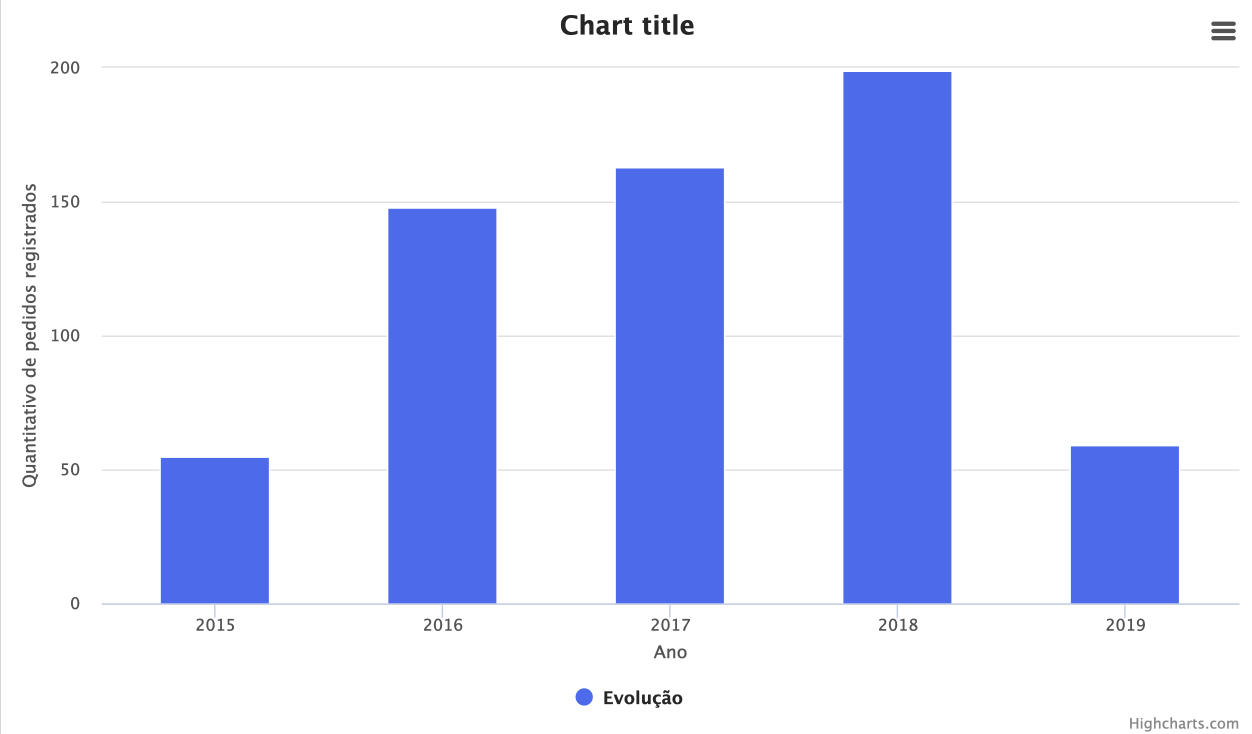
\includegraphics[width=400px]{/Users/ewersonpimenta/Desktop/ESIC_TCC/TCC_v2.1/RMARKDOWN/IMAGENS/Evolucao_pedidos}

\begin{Shaded}
\begin{Highlighting}[]
\NormalTok{summary(DB$DATA_REGISTRO)}
\NormalTok{class()}
\FunctionTok{inic = as.Date(min(DB$DATA_REGISTRO), format = "%m/%d/%y %H:}\AttributeTok{%M:%S", tz = "UTC")}
\NormalTok{fim = max(DB$DATA_REGISTRO), date_format())}
\NormalTok{cat(paste0(}\StringTok{"Período de pedidos registrados que serão utilizados nessa análise "}\NormalTok{, inic, }\StringTok{" até "}\NormalTok{, fim))}

\NormalTok{time_index_h <- seq(from = as.POSIXct(inic), }
\NormalTok{                  to = as.POSIXct(fim), by = }\StringTok{"hour"}\NormalTok{)}
\NormalTok{time_index_w <- weekdays(time_index_h)}
\CommentTok{# or}
\CommentTok{#time_index_w <- lubridate::wday(time_index_h)}
\NormalTok{library(lubridate)}
\FunctionTok{date<-ymd_hms(“2016-06-06 09:}\AttributeTok{45:12”)}
\NormalTok{wday(date)}
\end{Highlighting}
\end{Shaded}

\hypertarget{mineracao-de-texto}{%
\subsection{Mineração de texto}\label{mineracao-de-texto}}

\hypertarget{palavras-por-pedido}{%
\subsubsection{Palavras por pedido}\label{palavras-por-pedido}}

\begin{quote}
Análise2: distribuição de frequência de palavras por diretoria e algumas
estatísticas descritivas
\end{quote}

\hypertarget{ferramentas}{%
\paragraph{Ferramentas}\label{ferramentas}}

Iniciamos as manipulações utilizando recursos da função
\texttt{unnest\_tokens(\ )} do pacote \texttt{library(tidytext)} que nos
permite trabalhar com textos em um formato \texttt{tidy}, ou seja que
coloca uma palavra por linha em uma única coluna, formando, assim,
\emph{termos/palavras} por linha. Utilizamos, também, ainda os recursos
do pacote \texttt{library(diplyr)} para, posteriormente, agrupar esses
termos por diretoria e calcular a frequência dos \emph{termos}.

Verificamos que as 10 palavras mais frequentes em todos os pedidos
realizados são palavras sem acréscimo contextual, pois essas não
acrescentam nenhum sentido semântico como, por exemplo: preposições (de,
da, do, para, em, no), conjunção (e) e artigos(o,a).

Citar o que é preoposição.

\hypertarget{tabela3-palavras-mais-frequentes}{%
\paragraph{Tabela3: Palavras mais
frequentes}\label{tabela3-palavras-mais-frequentes}}

\begin{itemize}
\tightlist
\item
  Tabela 03 Palavras mais frequentes em todo o conjunto de solicitações
\end{itemize}

\begin{Shaded}
\begin{Highlighting}[]
\KeywordTok{library}\NormalTok{(tidytext)}
\NormalTok{palavras <-}\StringTok{ }\NormalTok{DB }\OperatorTok
\StringTok{  }\KeywordTok{unnest_tokens}\NormalTok{(palavra, PEDIDO) }\OperatorTok
\StringTok{  }\KeywordTok{count}\NormalTok{(palavra, }\DataTypeTok{sort =} \OtherTok{TRUE}\NormalTok{) }\OperatorTok
\StringTok{  }\KeywordTok{ungroup}\NormalTok{()}

\NormalTok{palavras[}\DecValTok{0}\OperatorTok{:}\DecValTok{10}\NormalTok{,] }\OperatorTok
\StringTok{  }\KeywordTok{kable}\NormalTok{(}\StringTok{"latex"}\NormalTok{, }\DataTypeTok{caption =} \StringTok{"Principais palavras com stopwords"}\NormalTok{, }
        \DataTypeTok{booktabs =}\NormalTok{ T, }\DataTypeTok{format.args =} \KeywordTok{list}\NormalTok{(}\DataTypeTok{decimal.mark =} \StringTok{','}\NormalTok{, }\DataTypeTok{big.mark =} \StringTok{"."}\NormalTok{)) }\OperatorTok
\StringTok{  }\KeywordTok{kable_styling}\NormalTok{(}\DataTypeTok{latex_options =} \KeywordTok{c}\NormalTok{(}\StringTok{"striped"}\NormalTok{, }\StringTok{"hold_position"}\NormalTok{))}
\end{Highlighting}
\end{Shaded}

\begin{table}[!h]

\caption{\label{tab:unnamed-chunk-30}Principais palavras com stopwords}
\centering
\begin{tabular}{lr}
\toprule
palavra & n\\
\midrule
\rowcolor{gray!6}  de & 4.071\\
a & 1.311\\
\rowcolor{gray!6}  e & 1.162\\
do & 900\\
\rowcolor{gray!6}  o & 891\\
\addlinespace
da & 821\\
\rowcolor{gray!6}  para & 712\\
no & 584\\
\rowcolor{gray!6}  em & 575\\
energia & 553\\
\bottomrule
\end{tabular}
\end{table}

\hypertarget{tabelas456-palavras-mais-frequentes-por-diretoria}{%
\paragraph{Tabelas4,5,6: Palavras mais frequentes por
diretoria}\label{tabelas456-palavras-mais-frequentes-por-diretoria}}

Cria o objeto de palavras por diretoria

\begin{Shaded}
\begin{Highlighting}[]
\NormalTok{palavras_diretoria <-}\StringTok{ }\NormalTok{DB }\OperatorTok
\StringTok{  }\KeywordTok{unnest_tokens}\NormalTok{(palavra, PEDIDO) }\OperatorTok
\StringTok{  }\KeywordTok{count}\NormalTok{(DIRETORIA,palavra, }\DataTypeTok{sort =} \OtherTok{TRUE}\NormalTok{) }\OperatorTok
\StringTok{  }\KeywordTok{ungroup}\NormalTok{() }\OperatorTok\StringTok{  }\KeywordTok{droplevels}\NormalTok{() }\OperatorTok\StringTok{ }\KeywordTok{drop_na}\NormalTok{()}

\NormalTok{palavras_diretoria}\OperatorTok{$}\NormalTok{DIRETORIA =}\StringTok{ }\KeywordTok{as.factor}\NormalTok{(palavras_diretoria}\OperatorTok{$}\NormalTok{DIRETORIA)}
\end{Highlighting}
\end{Shaded}

\hypertarget{tabelas4-palavras-mais-frequentes-dea}{%
\subparagraph{Tabelas4: Palavras mais frequentes
DEA}\label{tabelas4-palavras-mais-frequentes-dea}}

\begin{itemize}
\tightlist
\item
  Tabela 04 Palavras mais frequentes no conjunto de solicitações por
  diretoria
\end{itemize}

\begin{Shaded}
\begin{Highlighting}[]
\NormalTok{DEA_termo =}\StringTok{ }
\NormalTok{palavras_diretoria }\OperatorTok
\StringTok{  }\KeywordTok{filter}\NormalTok{(DIRETORIA }\OperatorTok{==}\StringTok{ "DEA"}\NormalTok{) }\OperatorTok\StringTok{ }\KeywordTok{droplevels}\NormalTok{()}

\NormalTok{DEA_termo }\OperatorTok
\StringTok{    }\KeywordTok{top_n}\NormalTok{(}\DataTypeTok{n =} \DecValTok{10}\NormalTok{) }\OperatorTok
\StringTok{  }\KeywordTok{kable}\NormalTok{(}\StringTok{"latex"}\NormalTok{, }\DataTypeTok{caption =} \StringTok{"Principais palavras com stopwords (DEA)"}\NormalTok{, }
        \DataTypeTok{booktabs =}\NormalTok{ T, }\DataTypeTok{format.args =} \KeywordTok{list}\NormalTok{(}\DataTypeTok{decimal.mark =} \StringTok{','}\NormalTok{, }\DataTypeTok{big.mark =} \StringTok{"."}\NormalTok{)) }\OperatorTok
\StringTok{  }\KeywordTok{kable_styling}\NormalTok{(}\DataTypeTok{latex_options =} \KeywordTok{c}\NormalTok{(}\StringTok{"striped"}\NormalTok{, }\StringTok{"hold_position"}\NormalTok{))}
\end{Highlighting}
\end{Shaded}

\begin{verbatim}
## Selecting by n
\end{verbatim}

\begin{table}[!h]

\caption{\label{tab:unnamed-chunk-32}Principais palavras com stopwords (DEA)}
\centering
\begin{tabular}{llr}
\toprule
\rowcolor{gray!6}  DIRETORIA & palavra & n\\


\bottomrule
\end{tabular}
\end{table}

\hypertarget{tabelas5-palavras-mais-frequentes-dee}{%
\subparagraph{Tabelas5: Palavras mais frequentes
DEE}\label{tabelas5-palavras-mais-frequentes-dee}}

\begin{itemize}
\tightlist
\item
  Tabela 05 Palavras mais frequentes no conjunto de solicitações por
  diretoria
\end{itemize}

\begin{Shaded}
\begin{Highlighting}[]
\NormalTok{DEE_termo =}\StringTok{ }
\NormalTok{palavras_diretoria }\OperatorTok
\StringTok{  }\KeywordTok{filter}\NormalTok{(DIRETORIA }\OperatorTok{==}\StringTok{ "DEE"}\NormalTok{) }\OperatorTok\StringTok{ }\KeywordTok{droplevels}\NormalTok{()}
  
\NormalTok{DEE_termo }\OperatorTok\StringTok{ }
\StringTok{    }\KeywordTok{top_n}\NormalTok{(}\DataTypeTok{n =} \DecValTok{10}\NormalTok{) }\OperatorTok
\StringTok{  }\KeywordTok{kable}\NormalTok{(}\StringTok{"latex"}\NormalTok{, }\DataTypeTok{caption =} \StringTok{"Principais palavras com stopwords (DEA)"}\NormalTok{, }
        \DataTypeTok{booktabs =}\NormalTok{ T, }\DataTypeTok{format.args =} \KeywordTok{list}\NormalTok{(}\DataTypeTok{decimal.mark =} \StringTok{','}\NormalTok{, }\DataTypeTok{big.mark =} \StringTok{"."}\NormalTok{)) }\OperatorTok
\StringTok{  }\KeywordTok{kable_styling}\NormalTok{(}\DataTypeTok{latex_options =} \KeywordTok{c}\NormalTok{(}\StringTok{"striped"}\NormalTok{, }\StringTok{"hold_position"}\NormalTok{))}
\end{Highlighting}
\end{Shaded}

\begin{verbatim}
## Selecting by n
\end{verbatim}

\begin{table}[!h]

\caption{\label{tab:unnamed-chunk-33}Principais palavras com stopwords (DEA)}
\centering
\begin{tabular}{llr}
\toprule
\rowcolor{gray!6}  DIRETORIA & palavra & n\\


\bottomrule
\end{tabular}
\end{table}

\hypertarget{tabelas6-palavras-mais-frequentes-outros}{%
\subparagraph{Tabelas6: Palavras mais frequentes
OUTROS}\label{tabelas6-palavras-mais-frequentes-outros}}

\begin{itemize}
\tightlist
\item
  Tabela 06 Palavras mais frequentes no conjunto de solicitações por
  diretoria
\end{itemize}

\begin{Shaded}
\begin{Highlighting}[]
\NormalTok{OUTROS =}\StringTok{ }
\NormalTok{palavras_diretoria }\OperatorTok
\StringTok{  }\KeywordTok{filter}\NormalTok{(DIRETORIA }\OperatorTok{==}\StringTok{ "OUTROS"}\NormalTok{) }\OperatorTok\StringTok{ }\KeywordTok{droplevels}\NormalTok{()}
  
\NormalTok{OUTROS }\OperatorTok
\StringTok{    }\KeywordTok{top_n}\NormalTok{(}\DataTypeTok{n =} \DecValTok{10}\NormalTok{) }\OperatorTok
\StringTok{  }\KeywordTok{kable}\NormalTok{(}\StringTok{"latex"}\NormalTok{, }\DataTypeTok{caption =} \StringTok{"Principais palavras com stopwords (OUTROS)"}\NormalTok{, }
        \DataTypeTok{booktabs =}\NormalTok{ T, }\DataTypeTok{format.args =} \KeywordTok{list}\NormalTok{(}\DataTypeTok{decimal.mark =} \StringTok{','}\NormalTok{, }\DataTypeTok{big.mark =} \StringTok{"."}\NormalTok{)) }\OperatorTok
\StringTok{  }\KeywordTok{kable_styling}\NormalTok{(}\DataTypeTok{latex_options =} \KeywordTok{c}\NormalTok{(}\StringTok{"striped"}\NormalTok{, }\StringTok{"hold_position"}\NormalTok{))}
\end{Highlighting}
\end{Shaded}

\begin{verbatim}
## Selecting by n
\end{verbatim}

\begin{table}[!h]

\caption{\label{tab:unnamed-chunk-34}Principais palavras com stopwords (OUTROS)}
\centering
\begin{tabular}{llr}
\toprule
DIRETORIA & palavra & n\\
\midrule
\rowcolor{gray!6}  OUTROS & de & 1.073\\
OUTROS & a & 384\\
\rowcolor{gray!6}  OUTROS & e & 359\\
OUTROS & o & 261\\
\rowcolor{gray!6}  OUTROS & da & 224\\
\addlinespace
OUTROS & do & 207\\
\rowcolor{gray!6}  OUTROS & para & 162\\
OUTROS & ou & 160\\
\rowcolor{gray!6}  OUTROS & em & 158\\
OUTROS & que & 152\\
\bottomrule
\end{tabular}
\end{table}

Mesmo assim, abrindo para cada uma das 3 possíveis cateogorias da
variável \textbf{Diretoria} temos que as principais palavras não agregam
nenhum valor semântico, exceto pela palavra energia que apareceu na
oitava e nona colocação de maior frequência dos documentos de pedidos
enviados à \emph{DEA} e \emph{DEE}, respectivamente. Isso devido ao
excesso de uso de \textbf{stop words} em textos humanos.

Em passos mais adiante serão removidas essas palavras, \textbf{stop
words}, e a partir da remoção o trabalho se dará apenas com palavras de
sentido semântico relevante aos subjetivos solicitados às diretorias,
acrescentando assim maior assertividade do modelo de classificação.

Verificamos, antes disso, o total, freq. e média de palavras por
diretoria, bem como comparações 2 a 2 para cada uma das categorias. E
avançamos um pouco com gráficos da contagem de frequência e a lei de
\textbf{Zipf} que dá suporte as conclusões do passo anterior e, a por
conseguinte, é definida a estatística de \textbf{tf\_idf} (\textbf{term
frequency times inverse document frequency}), uma estatística utilizada
para ressaltar termos relevantes para um documento em particular.

\hypertarget{analise2-comparacao-de-freq.-de-palavras-por-diretoria}{%
\subsubsection{Análise2: Comparação de freq. de palavras por
diretoria}\label{analise2-comparacao-de-freq.-de-palavras-por-diretoria}}

\begin{itemize}
\tightlist
\item
  Total de palavras por diretoria, total de pedidos por diretoria e
  número médio de palavras por pedido e diretoria
\end{itemize}

\begin{Shaded}
\begin{Highlighting}[]
\NormalTok{total_palavras =}\StringTok{ }\NormalTok{palavras_diretoria }\OperatorTok
\StringTok{  }\KeywordTok{group_by}\NormalTok{(DIRETORIA) }\OperatorTok
\StringTok{  }\KeywordTok{summarize}\NormalTok{(}\DataTypeTok{total_palavras =} \KeywordTok{sum}\NormalTok{(n))}

\NormalTok{total_palavras}\OperatorTok{$}\NormalTok{DIRETORIA =}\StringTok{ }\KeywordTok{as.character}\NormalTok{(total_palavras}\OperatorTok{$}\NormalTok{DIRETORIA)}
\NormalTok{total_palavras =}\StringTok{ }\KeywordTok{left_join}\NormalTok{(}\DataTypeTok{x =}\NormalTok{ total_palavras, }\DataTypeTok{y =}\NormalTok{ pedidos_diretoria1, }
                           \DataTypeTok{by =} \StringTok{"DIRETORIA"}\NormalTok{) }\OperatorTok
\KeywordTok{mutate}\NormalTok{(}\DataTypeTok{media_palavras_porpedidoEdiretoria =}\NormalTok{ total_palavras}\OperatorTok{/}\NormalTok{total_pedidos)}
\end{Highlighting}
\end{Shaded}

\hypertarget{tabelas7-total-de-palavras-por-diretoria-total-de-pedidos-por-diretoria-e-numero-medio-de-palavras-por-pedido-e-diretoria}{%
\paragraph{Tabelas7: Total de palavras por diretoria, total de pedidos
por diretoria e número médio de palavras por pedido e
diretoria}\label{tabelas7-total-de-palavras-por-diretoria-total-de-pedidos-por-diretoria-e-numero-medio-de-palavras-por-pedido-e-diretoria}}

\begin{itemize}
\tightlist
\item
  Total de palavras por diretoria, total de pedidos por diretoria e
  número médio de palavras por pedido e diretoria
\end{itemize}

\begin{Shaded}
\begin{Highlighting}[]
\NormalTok{total_palavras }\OperatorTok
\StringTok{  }\KeywordTok{kable}\NormalTok{(}\StringTok{"latex"}\NormalTok{, }\DataTypeTok{caption =} \StringTok{"Total de palavras, total de pedidos e número médio de palavras}
\StringTok{        por pedido e diretoria"}\NormalTok{, }
        \DataTypeTok{booktabs =}\NormalTok{ T, }\DataTypeTok{format.args =} \KeywordTok{list}\NormalTok{(}\DataTypeTok{decimal.mark =} \StringTok{','}\NormalTok{, }\DataTypeTok{big.mark =} \StringTok{"."}\NormalTok{)) }\OperatorTok
\StringTok{  }\KeywordTok{kable_styling}\NormalTok{(}\DataTypeTok{latex_options =} \KeywordTok{c}\NormalTok{(}\StringTok{"striped"}\NormalTok{, }\StringTok{"hold_position"}\NormalTok{))}
\end{Highlighting}
\end{Shaded}

\begin{table}[!h]

\caption{\label{tab:unnamed-chunk-36}Total de palavras, total de pedidos e número médio de palavras
        por pedido e diretoria}
\centering
\begin{tabular}{lrrr}
\toprule
DIRETORIA & total\_palavras & total\_pedidos & media\_palavras\_porpedidoEdiretoria\\
\midrule
\rowcolor{gray!6}  1 & 17.211 & 240 & 71,71250\\
2 & 15.536 & 244 & 63,67213\\
\rowcolor{gray!6}  5 & 3.619 & 67 & 54,01493\\
OUTROS & 13.351 & 154 & 86,69481\\
\bottomrule
\end{tabular}
\end{table}

Temos que o número médio de palavras por pedido é parecido entre as
diretorias. com médias de 55 palavras por pedido para DEE e 69,7 e 61,7,
respectivamente para DEA e OUTROS.

\hypertarget{figura1-distribuicao-de-frequencia-de-termos-por-diretoria}{%
\paragraph{Figura1: Distribuição de frequência de termos por
diretoria}\label{figura1-distribuicao-de-frequencia-de-termos-por-diretoria}}

\begin{itemize}
\tightlist
\item
  Distribuição da freq. de palavras usadas em solicitações por diretoria
  (histograma)
\end{itemize}

\begin{Shaded}
\begin{Highlighting}[]
\NormalTok{diretoria_palavras <-}\StringTok{ }\NormalTok{DB }\OperatorTok
\StringTok{  }\KeywordTok{unnest_tokens}\NormalTok{(palavra, PEDIDO) }\OperatorTok
\StringTok{  }\KeywordTok{count}\NormalTok{(DIRETORIA, palavra, }\DataTypeTok{sort =} \OtherTok{TRUE}\NormalTok{) }\OperatorTok
\StringTok{  }\KeywordTok{ungroup}\NormalTok{()}

\NormalTok{diretoria_palavras =}\StringTok{ }\KeywordTok{left_join}\NormalTok{(diretoria_palavras, total_palavras, }\DataTypeTok{by =} \StringTok{"DIRETORIA"}\NormalTok{)}

\KeywordTok{library}\NormalTok{(ggplot2)}
\NormalTok{gcomma <-}\StringTok{ }\ControlFlowTok{function}\NormalTok{(x) }\KeywordTok{format}\NormalTok{(x, }\DataTypeTok{big.mark =} \StringTok{"."}\NormalTok{, }\DataTypeTok{decimal.mark =} \StringTok{","}\NormalTok{, }\DataTypeTok{scientific =} \OtherTok{FALSE}\NormalTok{)}

\KeywordTok{ggplot}\NormalTok{(diretoria_palavras, }\KeywordTok{aes}\NormalTok{(n}\OperatorTok{/}\NormalTok{total_palavras, }\DataTypeTok{fill =}\NormalTok{ DIRETORIA)) }\OperatorTok{+}\StringTok{ }
\StringTok{  }\KeywordTok{geom_histogram}\NormalTok{(}\DataTypeTok{show.legend =} \OtherTok{FALSE}\NormalTok{) }\OperatorTok{+}\StringTok{ }\KeywordTok{xlim}\NormalTok{(}\OtherTok{NA}\NormalTok{, }\FloatTok{0.0021}\NormalTok{) }\OperatorTok{+}
\KeywordTok{facet_wrap}\NormalTok{(}\OperatorTok{~}\NormalTok{DIRETORIA, }\DataTypeTok{ncol =} \DecValTok{2}\NormalTok{, }\DataTypeTok{scales =} \StringTok{"free_y"}\NormalTok{) }\OperatorTok{+}\StringTok{ }
\StringTok{  }\KeywordTok{scale_y_continuous}\NormalTok{(}\DataTypeTok{labels=}\NormalTok{gcomma)  }\OperatorTok{+}
\StringTok{  }\KeywordTok{scale_x_continuous}\NormalTok{(}\DataTypeTok{labels=}\NormalTok{gcomma, }\DataTypeTok{limits =} \KeywordTok{c}\NormalTok{(}\OtherTok{NA}\NormalTok{, }\FloatTok{0.0021}\NormalTok{)) }\OperatorTok{+}
\StringTok{  }\KeywordTok{labs}\NormalTok{(}\DataTypeTok{y =} \StringTok{"frequência de termos"}\NormalTok{)}
\end{Highlighting}
\end{Shaded}

\begin{verbatim}
## Scale for 'x' is already present. Adding another scale for 'x', which
## will replace the existing scale.
\end{verbatim}

\begin{verbatim}
## `stat_bin()` using `bins = 30`. Pick better value with `binwidth`.
\end{verbatim}

\begin{verbatim}
## Warning: Removed 249 rows containing non-finite values (stat_bin).
\end{verbatim}

\begin{verbatim}
## Warning: Removed 4 rows containing missing values (geom_bar).
\end{verbatim}

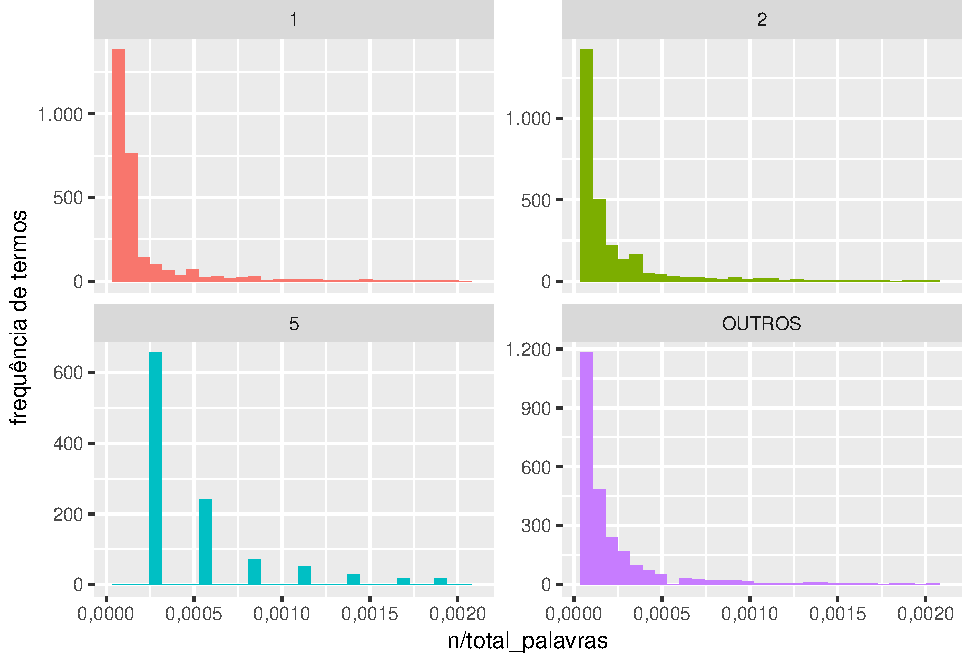
\includegraphics{markdown_v50_files/figure-latex/unnamed-chunk-37-1.pdf}

Pelos histogramas fica claro que as distribuições da frequência de
termos por diretoria possuem caudas mais alongadas à direita. Além
disso, algumas frequências não foram evidenciadas no gráfico por
questões de escala. De fato, as palavras/termos de maior recorrência nos
documentos/textos são as de menor relevância em contexto semântica.

Sabemos, portanto, que queremos encontrar valor exatamente nas partes
mais longas à direita das distribuições de frequência de termos, uma vez
que ali se encontram as palavras de maior relevância contextual.

Logo, a seguir, usamos da definição da lei \textbf{Zipf} que afirma que
a frequência que uma palavra (ou termo) aparece em um documento é
inversamente proporcional ao seu ranque.

\begin{quote}
lei de Zipf's
\end{quote}

Citar, aqui, ``There are very long tails to the right for these novels
(those extremely common words!) that we have not shown in these plots.
These plots exhibit similar distributions for all the novels, with many
words that occur rarely and fewer words that occur frequently.'' pág. 31
(Silge, Robinson). Que averigua que documentos de texto tendem a ter
distribuições de frequência de palavras similar, por conta das
stopwords.

Ainda de acordo com os autores, ``Distributions like those shown in
Figure 3-1 are typical in language. In fact, those types of long-tailed
distributions are so common in any given corpus of natural lan‐ guage
(like a book, or a lot of text from a website, or spoken words) that the
relation‐ ship between the frequency that a word is used and its rank
has been the subject of study.'' e por essa razão e a relação verificada
por George Zipf da relação inversa entre freq. de palavra e ranque
tiramos valor dos documentos partindo dessas premissas.

\begin{itemize}
\tightlist
\item
  Ranque de palavras pela pela lei de \textbf{Zipf}
\end{itemize}

\begin{Shaded}
\begin{Highlighting}[]
\NormalTok{freq_by_rank <-}\StringTok{ }\NormalTok{diretoria_palavras }\OperatorTok
\KeywordTok{group_by}\NormalTok{(DIRETORIA) }\OperatorTok
\KeywordTok{mutate}\NormalTok{(}\DataTypeTok{ranque =} \KeywordTok{row_number}\NormalTok{(),}
\StringTok{`}\DataTypeTok{frequência de termos}\StringTok{`}\NormalTok{ =}\StringTok{ }\NormalTok{n}\OperatorTok{/}\NormalTok{total_palavras)}
\end{Highlighting}
\end{Shaded}

\hypertarget{figura1-lei-de-zipf}{%
\paragraph{Figura1: Lei de Zipf}\label{figura1-lei-de-zipf}}

\begin{itemize}
\tightlist
\item
  Zipf's law
\end{itemize}

\begin{Shaded}
\begin{Highlighting}[]
\CommentTok{#plot1}
\NormalTok{freq_by_rank }\OperatorTok
\KeywordTok{ggplot}\NormalTok{(}\KeywordTok{aes}\NormalTok{(ranque, }\StringTok{`}\DataTypeTok{frequência de termos}\StringTok{`}\NormalTok{, }\DataTypeTok{color =}\NormalTok{ DIRETORIA)) }\OperatorTok{+}
\StringTok{  }\KeywordTok{geom_line}\NormalTok{(}\DataTypeTok{size =} \FloatTok{1.1}\NormalTok{, }\DataTypeTok{alpha =} \FloatTok{0.8}\NormalTok{, }\DataTypeTok{show.legend =} \OtherTok{FALSE}\NormalTok{) }\OperatorTok{+}\StringTok{ }\KeywordTok{scale_x_log10}\NormalTok{() }\OperatorTok{+}
\StringTok{  }\KeywordTok{scale_y_log10}\NormalTok{(}\DataTypeTok{labels=}\NormalTok{gcomma) }\OperatorTok{+}
\StringTok{  }\KeywordTok{scale_x_log10}\NormalTok{(}\DataTypeTok{labels=}\NormalTok{gcomma) }\OperatorTok{+}
\StringTok{  }\KeywordTok{labs}\NormalTok{(}\DataTypeTok{y =} \StringTok{"frequência de termos (log)"}\NormalTok{, }\DataTypeTok{x =} \StringTok{"ranque (log)"}\NormalTok{)}
\end{Highlighting}
\end{Shaded}

\begin{verbatim}
## Scale for 'x' is already present. Adding another scale for 'x', which
## will replace the existing scale.
\end{verbatim}

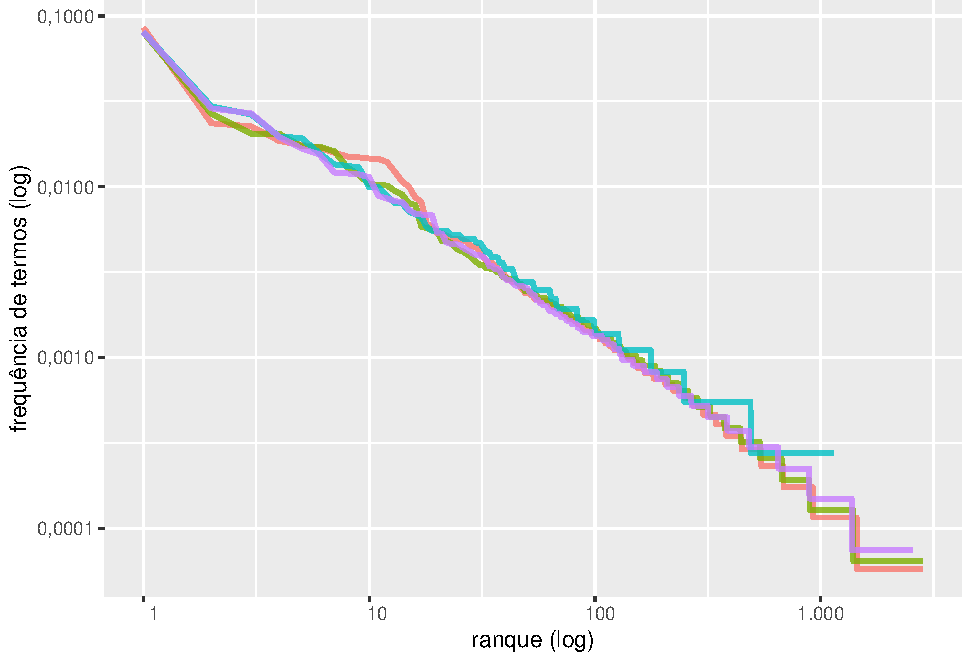
\includegraphics{markdown_v50_files/figure-latex/unnamed-chunk-39-1.pdf}

Vemos que exatamente nas extremidades do gráfico tem-se uma não
sobreposição de frequências por diretoria. Detalhe que o gráfico, em
questão, está na escala logarítmica no eixo x (ranque) e eixo y (freq.
de termos). Plotando desta forma, a relação inversamente proporcional
terá uma inclinação constante e negativa.

Tendo em vista, portanto, que o gráfico referido está em cordenadas
log-log e dado a semelhança de todos os documentos de texto das
diferentes diretorias, afirmamos que para todas as diretorias pela Lei
de \textbf{Zipf} a relação entre ranque e freq. de termos assumirá,
sempre, uma inclinação negativa, ou seja,

Daí, aplicando a escala log-log temos que e podemos aplicar um ajuste a
fim de encontrar um intercepto e coef. angular para traçar no gráfico
anterior.

\[
frequência \propto \frac{1}{ranque} \implies log(frequência) \propto log\left(\frac{1}{ranque}\right)
\]

Reescrever e exlicar a seguimentação em 3 partes como uma ``lei de
potenciacao dividida em 3 partes'' e então utilizar do seguimento do
meio, onde as freq. de ternos sao mais semelhantes para diferentes
ranques das diferentes diretorias. Fica claro pela eq.

``Notice that Figure 3-2 is in log-log coordinates. We see that all six
of Jane Austen's novels are similar to each other, and that the
relationship between rank and fre‐ quency does have negative slope. It
is not quite constant, though; perhaps we could view this as a broken
power law with, say, three sections. Let's see what the exponent of the
power law is for the middle section of the rank range.''

\begin{Shaded}
\begin{Highlighting}[]
\NormalTok{rank_subset <-}\StringTok{ }\NormalTok{freq_by_rank }\OperatorTok
\StringTok{      }\KeywordTok{filter}\NormalTok{(ranque }\OperatorTok{<}\StringTok{ }\DecValTok{500}\NormalTok{, ranque }\OperatorTok{>}\StringTok{ }\DecValTok{50}\NormalTok{)}

\NormalTok{(zipf_ajusteloglog <-}\StringTok{ }\KeywordTok{lm}\NormalTok{(}\KeywordTok{log10}\NormalTok{(}\StringTok{`}\DataTypeTok{frequência de termos}\StringTok{`}\NormalTok{) }\OperatorTok{~}\StringTok{ }\KeywordTok{log10}\NormalTok{(ranque), }
                         \DataTypeTok{data =}\NormalTok{ rank_subset))}
\end{Highlighting}
\end{Shaded}

\begin{verbatim}
## 
## Call:
## lm(formula = log10(`frequência de termos`) ~ log10(ranque), 
##     data = rank_subset)
## 
## Coefficients:
##   (Intercept)  log10(ranque)  
##       -1.0832        -0.8837
\end{verbatim}

Finalmente, traçando e sobrepondo o gráfico anterior com os valores de
initercepto e coeficiente angular obtidos no ajuste do passo anterior
temos a figura a seguir.

\hypertarget{figura1-lei-de-zipf-ajuste-log-log}{%
\paragraph{Figura1: Lei de Zipf + ajuste
log-log}\label{figura1-lei-de-zipf-ajuste-log-log}}

\begin{Shaded}
\begin{Highlighting}[]
\NormalTok{freq_by_rank }\OperatorTok
\KeywordTok{ggplot}\NormalTok{(}\KeywordTok{aes}\NormalTok{(ranque, }\StringTok{`}\DataTypeTok{frequência de termos}\StringTok{`}\NormalTok{, }\DataTypeTok{color =}\NormalTok{ DIRETORIA)) }\OperatorTok{+}
\KeywordTok{geom_abline}\NormalTok{(}\DataTypeTok{intercept =} \KeywordTok{coefficients}\NormalTok{(zipf_ajusteloglog)[}\DecValTok{1}\NormalTok{], }\DataTypeTok{slope =} \KeywordTok{coefficients}\NormalTok{(zipf_ajusteloglog)[}\DecValTok{2}\NormalTok{], }\DataTypeTok{color =} \StringTok{"gray50"}\NormalTok{, }\DataTypeTok{linetype =} \DecValTok{2}\NormalTok{) }\OperatorTok{+}
\KeywordTok{geom_line}\NormalTok{(}\DataTypeTok{size =} \FloatTok{1.1}\NormalTok{, }\DataTypeTok{alpha =} \FloatTok{0.8}\NormalTok{, }\DataTypeTok{show.legend =} \OtherTok{TRUE}\NormalTok{) }\OperatorTok{+}
\StringTok{  }\KeywordTok{scale_y_log10}\NormalTok{(}\DataTypeTok{labels=}\NormalTok{gcomma) }\OperatorTok{+}
\StringTok{  }\KeywordTok{scale_x_log10}\NormalTok{(}\DataTypeTok{labels=}\NormalTok{gcomma) }\OperatorTok{+}
\StringTok{  }\KeywordTok{labs}\NormalTok{(}\DataTypeTok{y =} \StringTok{"frequência de termos (log)"}\NormalTok{, }\DataTypeTok{x =} \StringTok{"ranque (log)"}\NormalTok{)}
\end{Highlighting}
\end{Shaded}

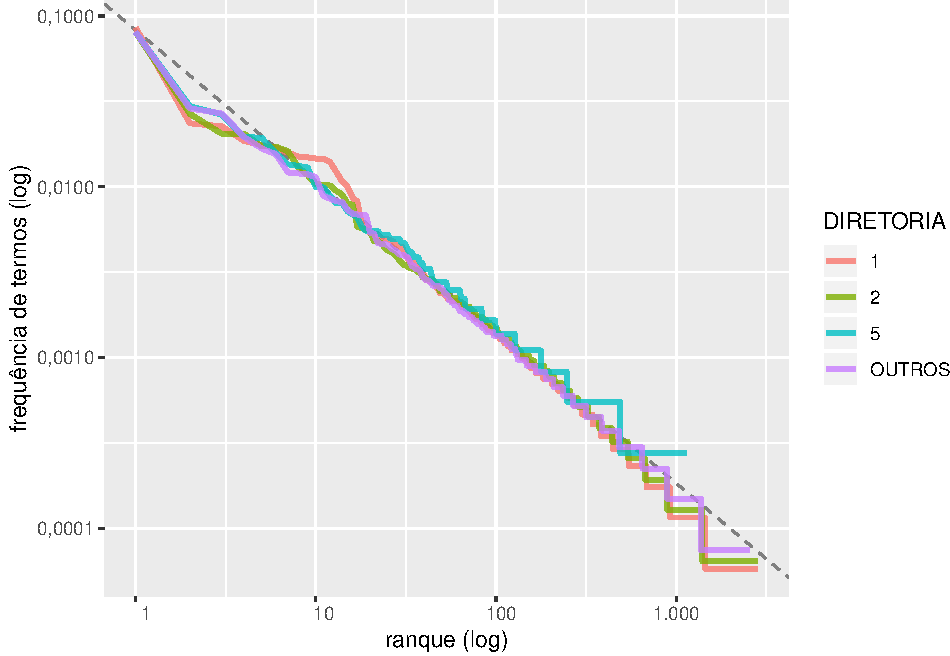
\includegraphics{markdown_v50_files/figure-latex/unnamed-chunk-41-1.pdf}

\hypertarget{the-bind-tf_idf}{%
\paragraph{\texorpdfstring{The Bind
\textbf{tf\_idf}}{The Bind tf\_idf}}\label{the-bind-tf_idf}}

Fundamentar o uso da estatística \textbf{tf\_idf}, bem como descrever a
definição.

\begin{quote}
The idea of tf-idf is to find the important words for the content of
each document by decreasing the weight for commonly used words and
increasing the weight for words that are not used very much in a
collection or corpus of documents, in this case, the group of Jane
Austen's novels as a whole. Calculating tf-idf attempts to find the
words that are important (i.e., common) in a text, but not too common.
Let's do that now. The bind\_tf\_idf function in the tidytext package
takes a tidy text dataset as input with one row per token (term), per
document. One column (word here) contains the terms/tokens, one column
contains the documents (book in this case), and the last necessary
column contains the counts, or how many times each document contains
each term (n in this example). We calculated a total for each book for
our explora‐ tions in previous sections, but it is not necessary for the
bind\_tf\_idf function; the table only needs to contain all the words in
each document.
\end{quote}

\begin{Shaded}
\begin{Highlighting}[]
\NormalTok{round_df <-}\StringTok{ }\ControlFlowTok{function}\NormalTok{(x, digits) \{}
    \CommentTok{# round all numeric variables}
    \CommentTok{# x: data frame }
    \CommentTok{# digits: number of digits to round}
\NormalTok{    numeric_columns <-}\StringTok{ }\KeywordTok{sapply}\NormalTok{(x, mode) }\OperatorTok{==}\StringTok{ 'numeric'}
\NormalTok{    x[numeric_columns] <-}\StringTok{  }\KeywordTok{round}\NormalTok{(x[numeric_columns], digits)}
\NormalTok{    x}
\NormalTok{\}}
\end{Highlighting}
\end{Shaded}

\begin{itemize}
\tightlist
\item
  Palavras mais relevantes de acordo com a estatística \textbf{tf\_idf}
\end{itemize}

\begin{Shaded}
\begin{Highlighting}[]
\NormalTok{diretoria_palavras_tfidf <-}\StringTok{ }\NormalTok{diretoria_palavras }\OperatorTok
\StringTok{  }\KeywordTok{bind_tf_idf}\NormalTok{(palavra, DIRETORIA, n) }\OperatorTok
\StringTok{  }\KeywordTok{select}\NormalTok{(}\OperatorTok{-}\NormalTok{total_palavras, }\OperatorTok{-}\NormalTok{total_pedidos, }\OperatorTok{-}\NormalTok{media_palavras_porpedidoEdiretoria) }\OperatorTok
\StringTok{  }\KeywordTok{arrange}\NormalTok{(}\KeywordTok{desc}\NormalTok{(tf_idf))}

\CommentTok{#options(digits=4)}
\KeywordTok{set.seed}\NormalTok{(}\DecValTok{7456}\NormalTok{)}
\NormalTok{amostra1 =}\StringTok{ }\KeywordTok{sample}\NormalTok{(}\KeywordTok{seq}\NormalTok{(}\DecValTok{1}\OperatorTok{:}\KeywordTok{dim}\NormalTok{(diretoria_palavras_tfidf)[}\DecValTok{1}\NormalTok{]), }\DecValTok{10}\NormalTok{, }\DataTypeTok{replace =} \OtherTok{FALSE}\NormalTok{)}
\KeywordTok{round_df}\NormalTok{(diretoria_palavras_tfidf[amostra1,],}\DecValTok{6}\NormalTok{)  }\OperatorTok
\StringTok{  }\KeywordTok{kable}\NormalTok{(}\StringTok{"latex"}\NormalTok{, }\DataTypeTok{caption =} \StringTok{"Total de palavras, total de pedidos e número médio de palavras }
\StringTok{        por pedido e diretoria"}\NormalTok{, }
        \DataTypeTok{booktabs =}\NormalTok{ T, }\DataTypeTok{format.args =} \KeywordTok{list}\NormalTok{(}\DataTypeTok{decimal.mark =} \StringTok{','}\NormalTok{, }\DataTypeTok{big.mark =} \StringTok{"."}\NormalTok{)) }\OperatorTok
\StringTok{  }\KeywordTok{kable_styling}\NormalTok{(}\DataTypeTok{latex_options =} \KeywordTok{c}\NormalTok{(}\StringTok{"striped"}\NormalTok{, }\StringTok{"hold_position"}\NormalTok{))}
\end{Highlighting}
\end{Shaded}

\begin{table}[!h]

\caption{\label{tab:unnamed-chunk-43}Total de palavras, total de pedidos e número médio de palavras 
        por pedido e diretoria}
\centering
\begin{tabular}{llrrrr}
\toprule
DIRETORIA & palavra & n & tf & idf & tf\_idf\\
\midrule
\rowcolor{gray!6}  1 & verão & 3 & 0,000174 & 1,386294 & 0,000242\\
1 & contratar & 1 & 0,000058 & 0,693147 & 0,000040\\
\rowcolor{gray!6}  5 & pública & 2 & 0,000553 & 0,000000 & 0,000000\\
2 & prezados & 58 & 0,003733 & 0,000000 & 0,000000\\
\rowcolor{gray!6}  5 & apresentação & 1 & 0,000276 & 0,693147 & 0,000192\\
\addlinespace
2 & coelba & 1 & 0,000064 & 0,693147 & 0,000045\\
\rowcolor{gray!6}  1 & fazendo & 9 & 0,000523 & 0,287682 & 0,000150\\
2 & power & 1 & 0,000064 & 1,386294 & 0,000089\\
\rowcolor{gray!6}  OUTROS & encontro & 1 & 0,000075 & 0,287682 & 0,000022\\
2 & prezado & 4 & 0,000257 & 0,287682 & 0,000074\\
\bottomrule
\end{tabular}
\end{table}

A estatística faz um trabalho brilhante ao ressaltar as palavras mais
relevantes dentro de cada conjunto de documentos (diretorias). As
tabelas a seguir mostram as 10 palavras mais relevantes de acordo com a
estatística tf\_idf por diretoria

\hypertarget{tabela8-top-12-termos-ordenados-pela-estatistica-tf_idf-dee}{%
\subparagraph{\texorpdfstring{Tabela8: top 12 termos ordenados pela
estatística \textbf{tf\_idf}
(DEE)}{Tabela8: top 12 termos ordenados pela estatística tf\_idf (DEE)}}\label{tabela8-top-12-termos-ordenados-pela-estatistica-tf_idf-dee}}

\begin{Shaded}
\begin{Highlighting}[]
\KeywordTok{round_df}\NormalTok{(diretoria_palavras_tfidf,}\DecValTok{5}\NormalTok{) }\OperatorTok
\StringTok{  }\KeywordTok{filter}\NormalTok{(DIRETORIA }\OperatorTok{==}\StringTok{ "DEE"}\NormalTok{) }\OperatorTok
\StringTok{  }\KeywordTok{top_n}\NormalTok{(}\DecValTok{12}\NormalTok{,tf_idf) }\OperatorTok
\StringTok{  }\KeywordTok{kable}\NormalTok{(}\StringTok{"latex"}\NormalTok{, }\DataTypeTok{caption =} \StringTok{"Top 10 termos (DEE)"}\NormalTok{, }
        \DataTypeTok{booktabs =}\NormalTok{ T, }\DataTypeTok{format.args =} \KeywordTok{list}\NormalTok{(}\DataTypeTok{decimal.mark =} \StringTok{','}\NormalTok{, }\DataTypeTok{big.mark =} \StringTok{"."}\NormalTok{)) }\OperatorTok
\StringTok{  }\KeywordTok{kable_styling}\NormalTok{(}\DataTypeTok{latex_options =} \KeywordTok{c}\NormalTok{(}\StringTok{"striped"}\NormalTok{, }\StringTok{"hold_position"}\NormalTok{))}
\end{Highlighting}
\end{Shaded}

\begin{table}[!h]

\caption{\label{tab:unnamed-chunk-44}Top 10 termos (DEE)}
\centering
\begin{tabular}{llrrrr}
\toprule
\rowcolor{gray!6}  DIRETORIA & palavra & n & tf & idf & tf\_idf\\


\bottomrule
\end{tabular}
\end{table}

\hypertarget{tabela9-top-12-termos-ordenados-pela-estatistica-tf_idf-dea}{%
\subparagraph{\texorpdfstring{Tabela9: top 12 termos ordenados pela
estatística \textbf{tf\_idf}
(DEA)}{Tabela9: top 12 termos ordenados pela estatística tf\_idf (DEA)}}\label{tabela9-top-12-termos-ordenados-pela-estatistica-tf_idf-dea}}

\begin{Shaded}
\begin{Highlighting}[]
\KeywordTok{round_df}\NormalTok{(diretoria_palavras_tfidf,}\DecValTok{5}\NormalTok{) }\OperatorTok
\StringTok{  }\KeywordTok{filter}\NormalTok{(DIRETORIA }\OperatorTok{==}\StringTok{ "DEA"}\NormalTok{) }\OperatorTok
\StringTok{  }\KeywordTok{top_n}\NormalTok{(}\DecValTok{12}\NormalTok{,tf_idf) }\OperatorTok
\StringTok{  }\KeywordTok{kable}\NormalTok{(}\StringTok{"latex"}\NormalTok{, }\DataTypeTok{caption =} \StringTok{"Top 10 termos (DEA)"}\NormalTok{, }
        \DataTypeTok{booktabs =}\NormalTok{ T, }\DataTypeTok{format.args =} \KeywordTok{list}\NormalTok{(}\DataTypeTok{decimal.mark =} \StringTok{','}\NormalTok{, }\DataTypeTok{big.mark =} \StringTok{"."}\NormalTok{)) }\OperatorTok
\StringTok{  }\KeywordTok{kable_styling}\NormalTok{(}\DataTypeTok{latex_options =} \KeywordTok{c}\NormalTok{(}\StringTok{"striped"}\NormalTok{, }\StringTok{"hold_position"}\NormalTok{))}
\end{Highlighting}
\end{Shaded}

\begin{table}[!h]

\caption{\label{tab:unnamed-chunk-45}Top 10 termos (DEA)}
\centering
\begin{tabular}{llrrrr}
\toprule
\rowcolor{gray!6}  DIRETORIA & palavra & n & tf & idf & tf\_idf\\


\bottomrule
\end{tabular}
\end{table}

\hypertarget{tabela10-top-10-termos-ordenados-pela-estatistica-tf_idf-outros}{%
\subparagraph{\texorpdfstring{Tabela10: top 10 termos ordenados pela
estatística \textbf{tf\_idf}
(OUTROS)}{Tabela10: top 10 termos ordenados pela estatística tf\_idf (OUTROS)}}\label{tabela10-top-10-termos-ordenados-pela-estatistica-tf_idf-outros}}

\begin{Shaded}
\begin{Highlighting}[]
\KeywordTok{round_df}\NormalTok{(diretoria_palavras_tfidf,}\DecValTok{5}\NormalTok{) }\OperatorTok
\StringTok{  }\KeywordTok{filter}\NormalTok{(DIRETORIA }\OperatorTok{==}\StringTok{ "OUTROS"}\NormalTok{) }\OperatorTok
\StringTok{  }\KeywordTok{top_n}\NormalTok{(}\DecValTok{12}\NormalTok{,tf_idf) }\OperatorTok
\StringTok{  }\KeywordTok{kable}\NormalTok{(}\StringTok{"latex"}\NormalTok{, }\DataTypeTok{caption =} \StringTok{"Top 10 termos (DEA)"}\NormalTok{, }
        \DataTypeTok{booktabs =}\NormalTok{ T, }\DataTypeTok{format.args =} \KeywordTok{list}\NormalTok{(}\DataTypeTok{decimal.mark =} \StringTok{','}\NormalTok{, }\DataTypeTok{big.mark =} \StringTok{"."}\NormalTok{)) }\OperatorTok
\StringTok{  }\KeywordTok{kable_styling}\NormalTok{(}\DataTypeTok{latex_options =} \KeywordTok{c}\NormalTok{(}\StringTok{"striped"}\NormalTok{, }\StringTok{"hold_position"}\NormalTok{))}
\end{Highlighting}
\end{Shaded}

\begin{table}[!h]

\caption{\label{tab:unnamed-chunk-46}Top 10 termos (DEA)}
\centering
\begin{tabular}{llrrrr}
\toprule
DIRETORIA & palavra & n & tf & idf & tf\_idf\\
\midrule
\rowcolor{gray!6}  OUTROS & funcionários & 37 & 0,00277 & 1,38629 & 0,00384\\
OUTROS & entidade & 27 & 0,00202 & 1,38629 & 0,00280\\
\rowcolor{gray!6}  OUTROS & contratos & 53 & 0,00397 & 0,69315 & 0,00275\\
OUTROS & empregados & 20 & 0,00150 & 1,38629 & 0,00208\\
\rowcolor{gray!6}  OUTROS & locação & 18 & 0,00135 & 1,38629 & 0,00187\\
\addlinespace
OUTROS & salários & 16 & 0,00120 & 1,38629 & 0,00166\\
\rowcolor{gray!6}  OUTROS & pessoal & 12 & 0,00090 & 1,38629 & 0,00125\\
OUTROS & cargos & 22 & 0,00165 & 0,69315 & 0,00114\\
\rowcolor{gray!6}  OUTROS & prestação & 11 & 0,00082 & 1,38629 & 0,00114\\
OUTROS & cargo & 20 & 0,00150 & 0,69315 & 0,00104\\
\addlinespace
\rowcolor{gray!6}  OUTROS & pagamento & 10 & 0,00075 & 1,38629 & 0,00104\\
OUTROS & passagens & 10 & 0,00075 & 1,38629 & 0,00104\\
\rowcolor{gray!6}  OUTROS & viagem & 10 & 0,00075 & 1,38629 & 0,00104\\
\bottomrule
\end{tabular}
\end{table}

Ou simplesmente verificamos através de um gráfico

\hypertarget{figura2-termos-mais-relevantes-por-diretoria-pela-estatistica-tf_idf}{%
\subparagraph{\texorpdfstring{Figura2: Termos mais relevantes por
diretoria pela estatística
\textbf{tf\_idf}}{Figura2: Termos mais relevantes por diretoria pela estatística tf\_idf}}\label{figura2-termos-mais-relevantes-por-diretoria-pela-estatistica-tf_idf}}

\begin{Shaded}
\begin{Highlighting}[]
\NormalTok{diretoria_palavras <-}\StringTok{ }\NormalTok{DB }\OperatorTok
\StringTok{  }\KeywordTok{unnest_tokens}\NormalTok{(palavra, PEDIDO) }\OperatorTok
\StringTok{  }\KeywordTok{count}\NormalTok{(DIRETORIA, palavra, }\DataTypeTok{sort =} \OtherTok{TRUE}\NormalTok{) }\OperatorTok
\StringTok{  }\KeywordTok{ungroup}\NormalTok{()}
\NormalTok{diretoria_palavras =}\StringTok{ }\KeywordTok{left_join}\NormalTok{(diretoria_palavras, total_palavras, }\DataTypeTok{by =} \StringTok{"DIRETORIA"}\NormalTok{)}
\end{Highlighting}
\end{Shaded}

\hypertarget{figura3-top-10-termos-por-diretoria-ordenados-pela-estatistica-tf_idf-e-com-stop-words-e-sem-stemming}{%
\subparagraph{\texorpdfstring{Figura3: Top 10 termos por diretoria
(ordenados pela estatística \textbf{tf\_idf} e com \textbf{stop words} e
sem
\textbf{stemming}}{Figura3: Top 10 termos por diretoria (ordenados pela estatística tf\_idf e com stop words e sem stemming}}\label{figura3-top-10-termos-por-diretoria-ordenados-pela-estatistica-tf_idf-e-com-stop-words-e-sem-stemming}}

\begin{Shaded}
\begin{Highlighting}[]
\NormalTok{plot_diretoria_palavras <-}\StringTok{ }\NormalTok{diretoria_palavras }\OperatorTok
\StringTok{  }\KeywordTok{bind_tf_idf}\NormalTok{(palavra, DIRETORIA, n) }\OperatorTok
\StringTok{  }\KeywordTok{arrange}\NormalTok{(}\KeywordTok{desc}\NormalTok{(tf_idf)) }\OperatorTok
\StringTok{  }\KeywordTok{mutate}\NormalTok{(}\DataTypeTok{palavra =} \KeywordTok{factor}\NormalTok{(palavra, }\DataTypeTok{levels =} \KeywordTok{rev}\NormalTok{(}\KeywordTok{unique}\NormalTok{(palavra)))) }\OperatorTok
\StringTok{  }\KeywordTok{mutate}\NormalTok{(}\DataTypeTok{DIRETORIA =} \KeywordTok{factor}\NormalTok{(DIRETORIA, }\DataTypeTok{levels =} \KeywordTok{c}\NormalTok{(}\StringTok{"DEA"}\NormalTok{,}\StringTok{"DEE"}\NormalTok{,}\StringTok{"OUTROS"}\NormalTok{)))}
\CommentTok{#View(head(plot_diretoria_palavras))}
\CommentTok{#jpeg("02_freq_palavras_dir.jpeg")}
\NormalTok{plot_diretoria_palavras }\OperatorTok
\StringTok{  }\KeywordTok{group_by}\NormalTok{(DIRETORIA) }\OperatorTok
\StringTok{  }\KeywordTok{top_n}\NormalTok{(}\DecValTok{10}\NormalTok{, tf_idf) }\OperatorTok
\StringTok{  }\KeywordTok{ungroup}\NormalTok{() }\OperatorTok
\StringTok{  }\KeywordTok{mutate}\NormalTok{(}\DataTypeTok{palavra =} \KeywordTok{reorder}\NormalTok{(palavra, tf_idf)) }\OperatorTok
\StringTok{  }\KeywordTok{ggplot}\NormalTok{(}\KeywordTok{aes}\NormalTok{(palavra, tf_idf, }\DataTypeTok{fill =}\NormalTok{ DIRETORIA)) }\OperatorTok{+}
\StringTok{  }\KeywordTok{geom_col}\NormalTok{(}\DataTypeTok{show.legend =} \OtherTok{FALSE}\NormalTok{) }\OperatorTok{+}
\StringTok{  }\KeywordTok{labs}\NormalTok{(}\DataTypeTok{x =} \OtherTok{NULL}\NormalTok{, }\DataTypeTok{y =} \StringTok{"tf-idf"}\NormalTok{) }\OperatorTok{+}
\StringTok{  }\KeywordTok{facet_wrap}\NormalTok{(}\OperatorTok{~}\NormalTok{DIRETORIA, }\DataTypeTok{ncol =} \DecValTok{2}\NormalTok{, }\DataTypeTok{scales =} \StringTok{"free"}\NormalTok{) }\OperatorTok{+}
\StringTok{  }\KeywordTok{coord_flip}\NormalTok{() }\OperatorTok{+}\StringTok{ }
\StringTok{  }\KeywordTok{scale_y_continuous}\NormalTok{(}\DataTypeTok{labels=}\NormalTok{gcomma)}
\end{Highlighting}
\end{Shaded}

\begin{verbatim}
## Warning: Factor `DIRETORIA` contains implicit NA, consider using
## `forcats::fct_explicit_na`
\end{verbatim}

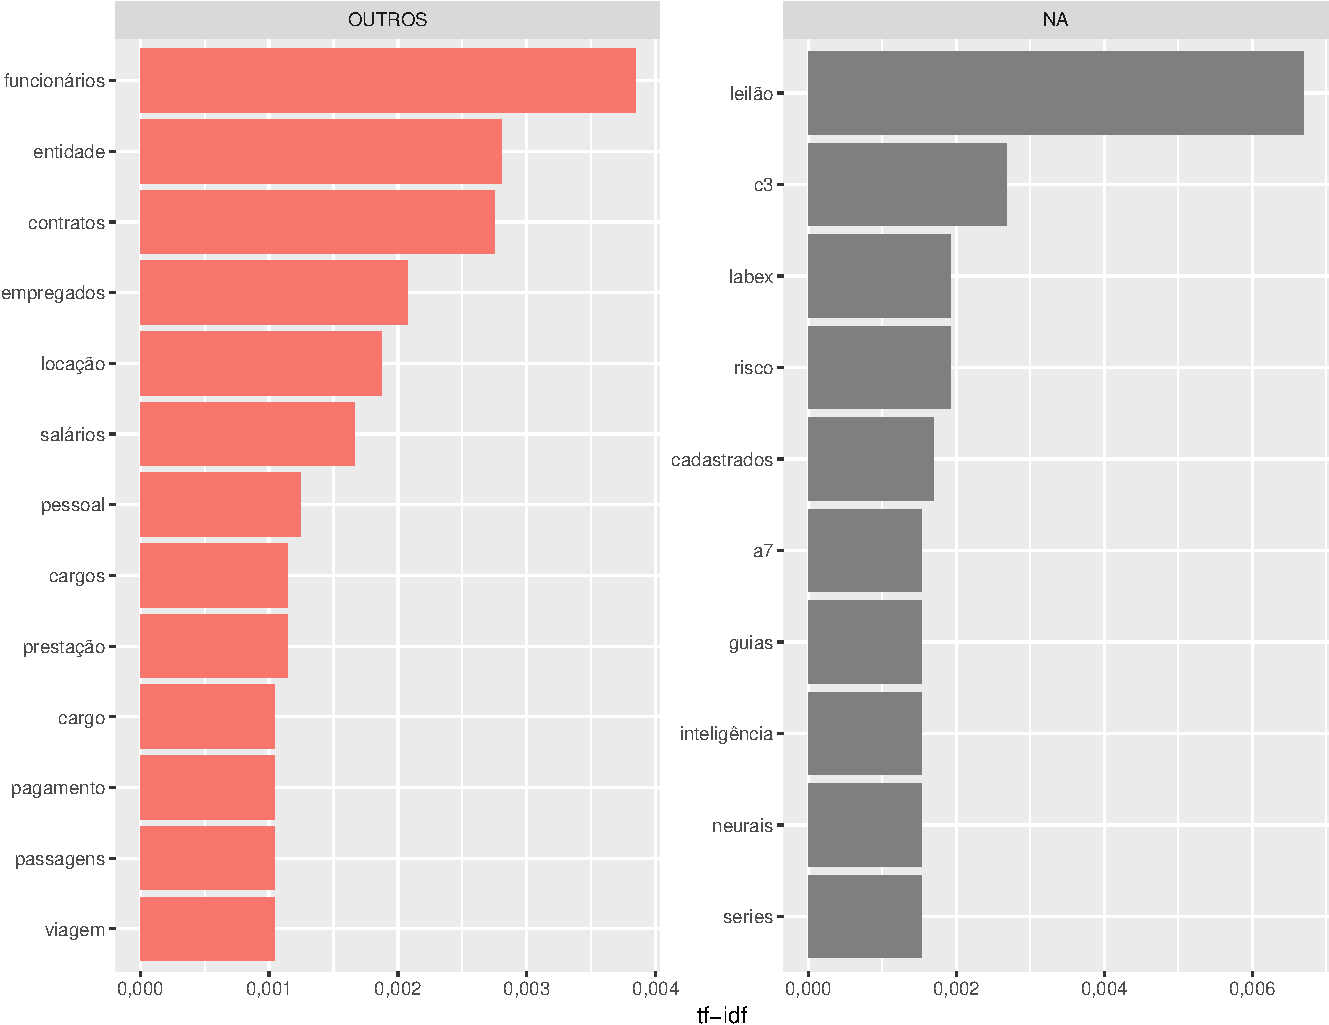
\includegraphics{markdown_v50_files/figure-latex/02_freq_palavras_dir-1.pdf}

\begin{Shaded}
\begin{Highlighting}[]
\CommentTok{#dev.off()}
\end{Highlighting}
\end{Shaded}

\hypertarget{filtrando-um-pedaco-de-texto}{%
\paragraph{Filtrando um pedaço de
texto}\label{filtrando-um-pedaco-de-texto}}

\begin{Shaded}
\begin{Highlighting}[]
\NormalTok{DB }\OperatorTok
\StringTok{  }\KeywordTok{filter}\NormalTok{(}\KeywordTok{str_detect}\NormalTok{(PEDIDO, }\StringTok{"in"}\NormalTok{)) }\OperatorTok
\StringTok{  }\KeywordTok{select}\NormalTok{(PEDIDO) }\OperatorTok
\StringTok{  }\KeywordTok{head}\NormalTok{()}
\end{Highlighting}
\end{Shaded}

\begin{verbatim}
## # A tibble: 6 x 1
##   PEDIDO                                                                   
##   <chr>                                                                    
## 1 "Empresa de Pesquisa Energética A Empresa de Pesquisa Energética (vincul~
## 2 Demanda ou carga Energética total (comercial, industrial, residencial e ~
## 3 "para EPE empresa de pesquisa energética - dados sobre custos de energia~
## 4 "Dados sobre Consumo de Energia por Unidades da Federação Boa tarde,\n\n~
## 5 Manifestação no processo de licenciamento da UHE Castanheira (processo n~
## 6 "Dados sobre quantidade de energia consumida e dinheiro pago pelo consum~
\end{verbatim}

Uma limpeza removendo palavras sem significado semântico (\textbf{stop
words}) pode auxiliar o algoritmo a retornar palavras ainda mais
acertivas, bem como o tratamento de \textbf{stemming}, abordados a
seguir.

Colocar tudo em minúsculo

\begin{Shaded}
\begin{Highlighting}[]
\NormalTok{DB}\OperatorTok{$}\NormalTok{PEDIDO1 =}\StringTok{ }\KeywordTok{tolower}\NormalTok{(DB}\OperatorTok{$}\NormalTok{PEDIDO)}
\end{Highlighting}
\end{Shaded}

\hypertarget{stopwords}{%
\subsubsection{Stopwords}\label{stopwords}}

Com o arquivo de \textbf{stop words} , vamos remover as palavras sem
sentido semântico

\begin{Shaded}
\begin{Highlighting}[]
\NormalTok{mystopwords <- data_frame(palavra = stopwords_pt)}
\FunctionTok{for (j in 1:}\AttributeTok{dim(DB)[1]) \{}
  \FunctionTok{for(i in 1:}\AttributeTok{dim(mystopwords)[1])\{}
\NormalTok{  stopw = as.character(mystopwords}\KeywordTok{[}\NormalTok{i}\KeywordTok{,}\NormalTok{1}\KeywordTok{]}\NormalTok{)}
\NormalTok{  DB$PEDIDO1}\KeywordTok{[}\NormalTok{j}\KeywordTok{]}\NormalTok{ = gsub(paste0(}\StringTok{"\textbackslash{}\textbackslash{} "}\NormalTok{,stopw,}\StringTok{" "}\NormalTok{), }\StringTok{" "}\NormalTok{, as.character(DB$PEDIDO1}\KeywordTok{[}\NormalTok{j}\KeywordTok{]}\NormalTok{))}
\NormalTok{\}}
\NormalTok{\}}
\end{Highlighting}
\end{Shaded}

Ou simplesmente

\begin{Shaded}
\begin{Highlighting}[]
\NormalTok{mystopwords <-}\StringTok{ }\KeywordTok{data_frame}\NormalTok{(}\DataTypeTok{palavra =}\NormalTok{ stopwords_pt)}
\end{Highlighting}
\end{Shaded}

\begin{verbatim}
## Warning: `data_frame()` is deprecated, use `tibble()`.
## This warning is displayed once per session.
\end{verbatim}

\begin{Shaded}
\begin{Highlighting}[]
\NormalTok{DB}\OperatorTok{$}\NormalTok{PEDIDO1 <-}\StringTok{ }\KeywordTok{removeWords}\NormalTok{(DB}\OperatorTok{$}\NormalTok{PEDIDO1, mystopwords}\OperatorTok{$}\NormalTok{palavra)}
\CommentTok{#View(head(DB))}
\end{Highlighting}
\end{Shaded}

\hypertarget{stemming}{%
\subsubsection{Stemming}\label{stemming}}

Podemos diminuir redundâncias por parte do algoritmo ensinando-o a
compreender palavras que podem estar escritas de forma diferente mas que
em significado semântico são semelhantes. Para isso, analisamos o
radical de palavras com um mesmo prefixo mas com sufixos diferentes seja
por quisistos como gênero ou plural.

Exemplos:

leilão \(\propto\) leilões estado \(\propto\) estados região \(\propto\)
regiões

Usando o pacote \texttt{ptstem}

\begin{Shaded}
\begin{Highlighting}[]
\KeywordTok{library}\NormalTok{(ptstem)}
\NormalTok{temp_stem1 =}\StringTok{ }\KeywordTok{proc.time}\NormalTok{()}
\NormalTok{stemming1 =}\StringTok{ }\KeywordTok{ptstem}\NormalTok{(DB}\OperatorTok{$}\NormalTok{PEDIDO1)}
\NormalTok{tempo_stem1 =}\StringTok{ }\KeywordTok{proc.time}\NormalTok{() }\OperatorTok{-}\StringTok{ }\NormalTok{temp_stem1}
\end{Highlighting}
\end{Shaded}

\begin{itemize}
\tightlist
\item
  Frequência de palavras por diretoria do stemming 1
\end{itemize}

\begin{Shaded}
\begin{Highlighting}[]
\NormalTok{diretoria_palavras_stem1 <-}\StringTok{ }\NormalTok{DB }\OperatorTok
\StringTok{  }\KeywordTok{mutate}\NormalTok{(}\DataTypeTok{PEDIDO1 =}\NormalTok{ stemming1) }\OperatorTok
\StringTok{  }\KeywordTok{unnest_tokens}\NormalTok{(palavra, PEDIDO1) }\OperatorTok
\StringTok{  }\KeywordTok{count}\NormalTok{(palavra, }\DataTypeTok{sort =} \OtherTok{TRUE}\NormalTok{) }\OperatorTok
\StringTok{  }\KeywordTok{ungroup}\NormalTok{()}
\end{Highlighting}
\end{Shaded}

\begin{Shaded}
\begin{Highlighting}[]
\KeywordTok{cat}\NormalTok{(}\KeywordTok{paste0}\NormalTok{(}\StringTok{"Utilizando o algoritmo de stemming do pacote 'ptstem' o número de palavras chaves sem stemming reduziu de "}\NormalTok{, }\KeywordTok{dim}\NormalTok{(diretoria_palavras)[}\DecValTok{1}\NormalTok{], }\StringTok{" para "}\NormalTok{, }\KeywordTok{dim}\NormalTok{(diretoria_palavras_stem1)[}\DecValTok{1}\NormalTok{], }\StringTok{", após stemming. Uma redução de "}\NormalTok{,}\KeywordTok{round}\NormalTok{(}\DecValTok{100}\OperatorTok{-}\KeywordTok{dim}\NormalTok{(diretoria_palavras_stem1)[}\DecValTok{1}\NormalTok{]}\OperatorTok{*}\DecValTok{100}\OperatorTok{/}\KeywordTok{dim}\NormalTok{(diretoria_palavras)[}\DecValTok{1}\NormalTok{],}\DecValTok{0}\NormalTok{),}\StringTok{"%."}\NormalTok{))}
\end{Highlighting}
\end{Shaded}

\begin{verbatim}
## Utilizando o algoritmo de stemming do pacote 'ptstem' o número de palavras chaves sem stemming reduziu de 9344 para 3244, após stemming. Uma redução de 65%.
\end{verbatim}

Usando o pacote \texttt{rslp}

\begin{Shaded}
\begin{Highlighting}[]
\KeywordTok{library}\NormalTok{(rslp)}
\NormalTok{temp_stem2 =}\StringTok{ }\KeywordTok{proc.time}\NormalTok{()}
\NormalTok{stemming2 =}\StringTok{ }\KeywordTok{rslp}\NormalTok{(DB}\OperatorTok{$}\NormalTok{PEDIDO1)}
\NormalTok{tempo_stem2 =}\StringTok{ }\KeywordTok{proc.time}\NormalTok{() }\OperatorTok{-}\StringTok{ }\NormalTok{temp_stem2}
\end{Highlighting}
\end{Shaded}

\begin{itemize}
\tightlist
\item
  Frequência de palavras por diretoria do stemming 2
\end{itemize}

\begin{Shaded}
\begin{Highlighting}[]
\NormalTok{diretoria_palavras_stem2 <-}\StringTok{ }\NormalTok{DB }\OperatorTok
\StringTok{  }\KeywordTok{mutate}\NormalTok{(}\DataTypeTok{PEDIDO1 =}\NormalTok{ stemming2) }\OperatorTok
\StringTok{  }\KeywordTok{unnest_tokens}\NormalTok{(palavra, PEDIDO1) }\OperatorTok
\StringTok{  }\KeywordTok{count}\NormalTok{(palavra, }\DataTypeTok{sort =} \OtherTok{TRUE}\NormalTok{) }\OperatorTok
\StringTok{  }\KeywordTok{ungroup}\NormalTok{()}
\end{Highlighting}
\end{Shaded}

\begin{Shaded}
\begin{Highlighting}[]
\KeywordTok{cat}\NormalTok{(}\KeywordTok{paste0}\NormalTok{(}\StringTok{"Utilizando o algoritmo de stemming do pacote 'rslp' o número de palavras chaves sem stemming reduziu de "}\NormalTok{, }\KeywordTok{dim}\NormalTok{(diretoria_palavras)[}\DecValTok{1}\NormalTok{], }\StringTok{" para "}\NormalTok{, }\KeywordTok{dim}\NormalTok{(diretoria_palavras_stem2)[}\DecValTok{1}\NormalTok{], }\StringTok{", após stemming. Uma redução de "}\NormalTok{, }\KeywordTok{round}\NormalTok{(}\DecValTok{100}\OperatorTok{-}\KeywordTok{dim}\NormalTok{(diretoria_palavras_stem2)[}\DecValTok{1}\NormalTok{]}\OperatorTok{*}\DecValTok{100}\OperatorTok{/}\KeywordTok{dim}\NormalTok{(diretoria_palavras)[}\DecValTok{1}\NormalTok{],}\DecValTok{0}\NormalTok{),}\StringTok{"%."}\NormalTok{))}
\end{Highlighting}
\end{Shaded}

\begin{verbatim}
## Utilizando o algoritmo de stemming do pacote 'rslp' o número de palavras chaves sem stemming reduziu de 9344 para 5235, após stemming. Uma redução de 44%.
\end{verbatim}

Uma redução considerável no número de termos ocorreu ao usar o algoritmo
\texttt{ptstem}, cerca de \(61\%\) de redução de termos versus \(36\%\)
utilziando o algoritmo \texttt{rslp}, ou seja, o algoritmo ptstem foi
mais eficiente na tarefa de agrupar os semelhantes (termos únicos).

Vale ressaltar, tabmbém, o tempo de processamento que ambos os
algoritmos requerem.

\begin{Shaded}
\begin{Highlighting}[]
\KeywordTok{cat}\NormalTok{(}\KeywordTok{paste0}\NormalTok{(}\StringTok{"O tempo de processamento do stemming rslp( ) foi de "}\NormalTok{,}\KeywordTok{round}\NormalTok{(tempo_stem1[}\DecValTok{3}\NormalTok{],}\DecValTok{2}\NormalTok{), }\StringTok{' segundos decorridos.'}\NormalTok{))}
\end{Highlighting}
\end{Shaded}

\begin{verbatim}
## O tempo de processamento do stemming rslp( ) foi de 10.51 segundos decorridos.
\end{verbatim}

\begin{Shaded}
\begin{Highlighting}[]
\KeywordTok{remove}\NormalTok{(tempo_stem1)}
\end{Highlighting}
\end{Shaded}

\begin{Shaded}
\begin{Highlighting}[]
\KeywordTok{cat}\NormalTok{(}\KeywordTok{paste0}\NormalTok{(}\StringTok{"O tempo de processamento do stemming rslp( ) foi de "}\NormalTok{,}\KeywordTok{round}\NormalTok{(tempo_stem2[}\DecValTok{3}\NormalTok{],}\DecValTok{2}\NormalTok{), }\StringTok{' segundos decorridos.'}\NormalTok{))}
\end{Highlighting}
\end{Shaded}

\begin{verbatim}
## O tempo de processamento do stemming rslp( ) foi de 0.82 segundos decorridos.
\end{verbatim}

\begin{Shaded}
\begin{Highlighting}[]
\KeywordTok{remove}\NormalTok{(tempo_stem2)}
\end{Highlighting}
\end{Shaded}

O tempo decorrido para processamento do algoritmo do \texttt{ptstem} foi
de aproximadamente 12 segundos versus 1 segundo decorrido para o
processamento do algoritmo do \texttt{rslp}. Logo, o \texttt{rslp} é
quase 12 vezes mais eficiente em termos de tempo de processamento. Além
disso, o \texttt{rslp} remove acentuações e caracteres como ``ç''. Isso
irá nos ajudar mais a frente quando utilizarmos os principais termos
como variáveis binárias e preditoras do modelo de classificação.

Entretanto, o algoritmo mais lento, \texttt{ptstem}, foi mais
interessante em termos de redução do número de termos únicos, cerca de
\(25\%\) menos termos únicos em relação ao outro algoritmo. Além disso,
por se tratar de uma base de dados relativamente pequena, 625 pedidos, e
pouco mais de 4 mil termos únicos em todo o conjunto de texto, além
disso vamos utilizar de um alto poder de processamento da máquina no
referido estudo. Optamos, portanto, por utilizar ambos algoritmos.
Vamos, primeiro, aplicar o removedor de sufixos da lingua portuguesa
\texttt{rslp} seguido do \texttt{ptstem}.

Comparação do texto original c/ os 2 algoritmos e o final implementados
após diferentes \textbf{stemmings}

\begin{Shaded}
\begin{Highlighting}[]
\NormalTok{DB}\OperatorTok{$}\NormalTok{PEDIDO[}\DecValTok{227}\NormalTok{]}
\end{Highlighting}
\end{Shaded}

\begin{verbatim}
## [1] "Destino dos honorários sucumbências Prezados, boa tarde. Desejo obter informações acerca da destinação dada aos honorários de sucumbência no âmbito desta empresa. Caso eles sejam repartidos entre os advogados de carreira integrantes do quadro de pessoal, desejo ter acesso à norma e/ou regulamento da empresa que trate do assunto. Desde já agradeço."
\end{verbatim}

\begin{Shaded}
\begin{Highlighting}[]
\CommentTok{#stemming1[227]}
\CommentTok{#stemming2[227]}
\NormalTok{DB}\OperatorTok{$}\NormalTok{PEDIDO1[}\DecValTok{227}\NormalTok{]}
\end{Highlighting}
\end{Shaded}

\begin{verbatim}
## [1] "destino  honorários sucumbências ,  . desejo obter    destinação dada  honorários  sucumbência  âmbito  empresa.    repartidos   advogados  carreira integrantes  quadro  pessoal, desejo    norma / regulamento  empresa  trate  assunto.   ."
\end{verbatim}

\begin{Shaded}
\begin{Highlighting}[]
\NormalTok{DB}\OperatorTok{$}\NormalTok{PEDIDO[}\DecValTok{350}\NormalTok{]}
\end{Highlighting}
\end{Shaded}

\begin{verbatim}
## [1] "SOLICITAÇÃO DE NOTAS TÉCNICAS Prezados(as) Senhores(as),\n\nsou o Eng° Eletricista Lidinei Sergio Mesquita Neri (ex-Colaborador da ELETROBRAS ELETRONUCLEAR).\n\nSolicito a gentileza de informar de que forma poderei conseguir, para informação e estudo, cópias impressas ou eletrônicas das seguintes Notas Técnicas:\n\n1) Demanda de Energia - 2050\n\n2) Recursos Energéticos - 2050\n\n3) Oferta de Combustíveis - 2050\n\n4) Oferta de Eletricidade - 2050\n\nEsses 4 (quatro) documentos juntamente com o documento \"Cenário Econômico - 2050\" (que já possuo) constituem o Plano Nacional de Energia - 2050.\n\nDesde já, agradeço ao atendimento.\n\nAtenciosamente\n\nEng° Lidinei Sergio Mesquita Neri"
\end{verbatim}

\begin{Shaded}
\begin{Highlighting}[]
\CommentTok{#stemming1[350]}
\CommentTok{#stemming2[350]}
\NormalTok{DB}\OperatorTok{$}\NormalTok{PEDIDO1[}\DecValTok{350}\NormalTok{]}
\end{Highlighting}
\end{Shaded}

\begin{verbatim}
## [1] "  notas técnicas () senhores(),\n\n  eng° eletricista lidinei sergio mesquita neri (ex-colaborador  eletrobras eletronuclear).\n\n  gentileza  informar    poderei conseguir,    estudo, cópias impressas  eletrônicas  seguintes notas técnicas:\n\n) demanda   - 2050\n\n) recursos energéticos - 2050\n\n) oferta  combustíveis - 2050\n\n) oferta  eletricidade - 2050\n\n  () documentos juntamente   documento \"cenário econômico - 2050\" (  possuo) constituem  plano nacional   - 2050.\n\n ,   atendimento.\n\natenciosamente\n\neng° lidinei sergio mesquita neri"
\end{verbatim}

\begin{Shaded}
\begin{Highlighting}[]
\NormalTok{DB}\OperatorTok{$}\NormalTok{PEDIDO[}\DecValTok{615}\NormalTok{]}
\end{Highlighting}
\end{Shaded}

\begin{verbatim}
## [1] "Gás do pré-sal Com fundamento na Lei 12.527/2011 (Lei de Acesso a\nInformações Públicas) venho a requerer o acesso, em até 20 dias corridos (artigo 11, parágrafo 1º da Lei 12.527/11), aos seguintes dados:\n\n- Previsão de qual será o custo da energia de eventuais usinas térmicas movidas a gás natural do pré-sal, em R$/MWh, considerando o custo final do gás (incluindo extração, transporte desse gás etc). \n\nSolicito que as informações sejam fornecidas em formato digital,\nquando disponíveis, conforme estabelece o artigo 11, parágrafo 5º\nda lei 12.527/2011.\nNa eventualidade de as informações solicitadas não serem\nfornecidas, requeiro que seja apontada a razão da negativa bem\ncomo, se for o caso, eventual grau de classificação de sigilo\n(ultrassecreto, secreto ou reservado), tudo nos termos do artigo\n24, parágrafo 1º da Lei 12.527/2011.\nDesde logo agradeço pela atenção e peço deferimento."
\end{verbatim}

\begin{Shaded}
\begin{Highlighting}[]
\CommentTok{#stemming1[615]}
\CommentTok{#stemming2[615]}
\NormalTok{DB}\OperatorTok{$}\NormalTok{PEDIDO1[}\DecValTok{615}\NormalTok{]}
\end{Highlighting}
\end{Shaded}

\begin{verbatim}
## [1] "gás  pré-sal  fundamento  lei 12.527/2011 (lei   \n públicas)   requerer  ,   20 dias corridos (artigo 11, parágrafo 1º  lei 12.527/11),  seguintes :\n\n- previsão     custo    eventuais usinas térmicas movidas  gás natural  pré-sal,  $/mwh, considerando  custo   gás (incluindo extração, transporte  gás etc). \n\n     fornecidas   digital,\n disponíveis,  estabelece  artigo 11, parágrafo 5º\n lei 12.527/2011.\n eventualidade    solicitadas  serem\nfornecidas,    apontada  razão  negativa \n,    , eventual grau  classificação  sigilo\n(ultrassecreto, secreto  reservado),   termos  artigo\n24, parágrafo 1º  lei 12.527/2011.\n    atenção  peço deferimento."
\end{verbatim}

\begin{Shaded}
\begin{Highlighting}[]
\NormalTok{DB}\OperatorTok{$}\NormalTok{PEDIDO[}\DecValTok{617}\NormalTok{]}
\end{Highlighting}
\end{Shaded}

\begin{verbatim}
## [1] "Questionamento sobre dados do PIB apresentados em Planos Decenais de Expansão Energética (PDEs) publicados pela EPE. Gostaria de explicações sobre alguns valores da taxa de crescimento do PIB Nacional apresentados em alguns PDEs já publicados pela EPE.\nPor exemplo, na tabela 10 do PDE 2008-2017 (pag 34) é apresentado um valor histórico dos últimos 5 anos (2003 a 2007) de 3,2% a.a.. Já na tabela 1 do PDE 2023 (pag 17) é apresentado um valor histórico para o mesmo período, de 4% a.a.\nOutro exemplo pode ser visto na tabela 4 do PDE 2019 (pag 20) apresentando histórico para o período de 2004 a 2008, um valor de 4,7% a.a.; e na tabela 1 do PDE 2024 (pag 20), para o mesmo período, um valor de 4,8% a.a..\n \nVisto que se tratam de dados históricos, de períodos já passados, gostaria de saber o porquê destas divergências de valores.\n \nNo aguardo."
\end{verbatim}

\begin{Shaded}
\begin{Highlighting}[]
\CommentTok{#stemming1[617]}
\CommentTok{#stemming2[617]}
\NormalTok{DB}\OperatorTok{$}\NormalTok{PEDIDO1[}\DecValTok{617}\NormalTok{]}
\end{Highlighting}
\end{Shaded}

\begin{verbatim}
## [1] "questionamento    pib apresentados  planos decenais  expansão energética (pdes) publicados  .   explicações   valores  taxa  crescimento  pib nacional apresentados   pdes  publicados  .\n ,  tabela 10  pde 2008-2017 (pag 34)  apresentado   histórico  últimos   (2003  2007)  ,% ...   tabela   pde 2023 (pag 17)  apresentado   histórico    período,  % ..\n    visto  tabela   pde 2019 (pag 20) apresentando histórico   período  2004  2008,    ,% ..;   tabela   pde 2024 (pag 20),    período,    ,% ...\n \nvisto   tratam   históricos,  períodos  passados,       divergências  valores.\n \n aguardo."
\end{verbatim}

\begin{Shaded}
\begin{Highlighting}[]
\NormalTok{DB}\OperatorTok{$}\NormalTok{PEDIDO[}\DecValTok{619}\NormalTok{]}
\end{Highlighting}
\end{Shaded}

\begin{verbatim}
## [1] "Dados distribuição de energia- UF Amapá Verifiquei que no Plano Decenal de Expansão de Energia (2006/ 2015) tem uma tabela 2-25 - \"Brasil - Consumo de Energia Elétrica por Classe (GWh) – Trajetória de Referência\" (p. 44).\n\nPergunto se teriam essas informações sobre consumo por unidade de federação, caso específico no Amapá? Ou informações sobre distribuição de energia por setor produtivo nas unidades de federação?"
\end{verbatim}

\begin{Shaded}
\begin{Highlighting}[]
\CommentTok{#stemming1[619]}
\CommentTok{#stemming2[619]}
\NormalTok{DB}\OperatorTok{$}\NormalTok{PEDIDO1[}\DecValTok{619}\NormalTok{]}
\end{Highlighting}
\end{Shaded}

\begin{verbatim}
## [1] " distribuição  - uf amapá verifiquei   plano decenal  expansão   (2006/ 2015)   tabela -25 - \" - consumo   elétrica  classe (gwh) – trajetória  referência\" (. 44).\n\n      consumo  unidade  federação,  específico  amapá?    distribuição    setor produtivo  unidades  federação?"
\end{verbatim}

Cria, antes, uma variáveil PEDIDO1 que repete os passos feitos aos
termos quanto ao stemming so que no texto fonte.

\begin{Shaded}
\begin{Highlighting}[]
\NormalTok{DB}\OperatorTok{$}\NormalTok{PEDIDO1 =}\StringTok{ }\KeywordTok{tolower}\NormalTok{(DB}\OperatorTok{$}\NormalTok{PEDIDO)}
\NormalTok{mystopwords <-}\StringTok{ }\KeywordTok{data_frame}\NormalTok{(}\DataTypeTok{palavra =}\NormalTok{ stopwords_pt)}
\NormalTok{DB}\OperatorTok{$}\NormalTok{PEDIDO1 <-}\StringTok{ }\KeywordTok{removeWords}\NormalTok{(DB}\OperatorTok{$}\NormalTok{PEDIDO1, mystopwords}\OperatorTok{$}\NormalTok{palavra) }\CommentTok{# Remove Stop Words}
\NormalTok{DB}\OperatorTok{$}\NormalTok{PEDIDO1 <-}\StringTok{ }\KeywordTok{removePunctuation}\NormalTok{(DB}\OperatorTok{$}\NormalTok{PEDIDO1) }\CommentTok{# Remove Punctuation}
 
\NormalTok{rm_accent <-}\StringTok{ }\ControlFlowTok{function}\NormalTok{(str,}\DataTypeTok{pattern=}\StringTok{"all"}\NormalTok{) \{ }
   \ControlFlowTok{if}\NormalTok{(}\OperatorTok{!}\KeywordTok{is.character}\NormalTok{(str))}
\NormalTok{    str <-}\StringTok{ }\KeywordTok{as.character}\NormalTok{(str)}

\NormalTok{  pattern <-}\StringTok{ }\KeywordTok{unique}\NormalTok{(pattern)}

  \ControlFlowTok{if}\NormalTok{(}\KeywordTok{any}\NormalTok{(pattern}\OperatorTok{==}\StringTok{"Ç"}\NormalTok{))}
\NormalTok{    pattern[pattern}\OperatorTok{==}\StringTok{"Ç"}\NormalTok{] <-}\StringTok{ "ç"}

\NormalTok{  symbols <-}\StringTok{ }\KeywordTok{c}\NormalTok{(}
    \DataTypeTok{acute =} \StringTok{"áéíóúÁÉÍÓÚýÝ"}\NormalTok{,}
    \DataTypeTok{grave =} \StringTok{"àèìòùÀÈÌÒÙ"}\NormalTok{,}
    \DataTypeTok{circunflex =} \StringTok{"âêîôûÂÊÎÔÛ"}\NormalTok{,}
    \DataTypeTok{tilde =} \StringTok{"ãõÃÕñÑ"}\NormalTok{,}
    \DataTypeTok{umlaut =} \StringTok{"äëïöüÄËÏÖÜÿ"}\NormalTok{,}
    \DataTypeTok{cedil =} \StringTok{"çÇ"}
\NormalTok{  )}

\NormalTok{  nudeSymbols <-}\StringTok{ }\KeywordTok{c}\NormalTok{(}
    \DataTypeTok{acute =} \StringTok{"aeiouAEIOUyY"}\NormalTok{,}
    \DataTypeTok{grave =} \StringTok{"aeiouAEIOU"}\NormalTok{,}
    \DataTypeTok{circunflex =} \StringTok{"aeiouAEIOU"}\NormalTok{,}
    \DataTypeTok{tilde =} \StringTok{"aoAOnN"}\NormalTok{,}
    \DataTypeTok{umlaut =} \StringTok{"aeiouAEIOUy"}\NormalTok{,}
    \DataTypeTok{cedil =} \StringTok{"cC"}
\NormalTok{  )}

\NormalTok{  accentTypes <-}\StringTok{ }\KeywordTok{c}\NormalTok{(}\StringTok{"´"}\NormalTok{,}\StringTok{"`"}\NormalTok{,}\StringTok{"^"}\NormalTok{,}\StringTok{"~"}\NormalTok{,}\StringTok{"¨"}\NormalTok{,}\StringTok{"ç"}\NormalTok{)}

  \ControlFlowTok{if}\NormalTok{(}\KeywordTok{any}\NormalTok{(}\KeywordTok{c}\NormalTok{(}\StringTok{"all"}\NormalTok{,}\StringTok{"al"}\NormalTok{,}\StringTok{"a"}\NormalTok{,}\StringTok{"todos"}\NormalTok{,}\StringTok{"t"}\NormalTok{,}\StringTok{"to"}\NormalTok{,}\StringTok{"tod"}\NormalTok{,}\StringTok{"todo"}\NormalTok{)}\OperatorTok\NormalTok{pattern)) }\CommentTok{# opcao retirar todos}
    \KeywordTok{return}\NormalTok{(}\KeywordTok{chartr}\NormalTok{(}\KeywordTok{paste}\NormalTok{(symbols, }\DataTypeTok{collapse=}\StringTok{""}\NormalTok{), }\KeywordTok{paste}\NormalTok{(nudeSymbols, }\DataTypeTok{collapse=}\StringTok{""}\NormalTok{), str))}

  \ControlFlowTok{for}\NormalTok{(i }\ControlFlowTok{in} \KeywordTok{which}\NormalTok{(accentTypes}\OperatorTok\NormalTok{pattern))}
\NormalTok{    str <-}\StringTok{ }\KeywordTok{chartr}\NormalTok{(symbols[i],nudeSymbols[i], str) }

  \KeywordTok{return}\NormalTok{(str)}
\NormalTok{\}}


\NormalTok{DB}\OperatorTok{$}\NormalTok{PEDIDO1 <-}\StringTok{ }\KeywordTok{rm_accent}\NormalTok{(DB}\OperatorTok{$}\NormalTok{PEDIDO1) }\CommentTok{# Remove accent patterns}
\CommentTok{#View(head(DB))}
\CommentTok{#View(DB$PEDIDO1)}
\end{Highlighting}
\end{Shaded}

\begin{Shaded}
\begin{Highlighting}[]
\CommentTok{#View(head(DB))}
\CommentTok{### CARACTERES}
\NormalTok{DB}\OperatorTok{$}\NormalTok{PEDIDO1 =}\StringTok{ }\KeywordTok{gsub}\NormalTok{(}\StringTok{"-"}\NormalTok{,}\StringTok{" "}\NormalTok{,DB}\OperatorTok{$}\NormalTok{PEDIDO1)}
\NormalTok{DB}\OperatorTok{$}\NormalTok{PEDIDO1 =}\StringTok{ }\KeywordTok{gsub}\NormalTok{(}\StringTok{"[:.:]"}\NormalTok{,}\StringTok{""}\NormalTok{,DB}\OperatorTok{$}\NormalTok{PEDIDO1)}
\NormalTok{DB}\OperatorTok{$}\NormalTok{PEDIDO1 =}\StringTok{ }\KeywordTok{gsub}\NormalTok{(}\StringTok{"[:,:]"}\NormalTok{,}\StringTok{""}\NormalTok{,DB}\OperatorTok{$}\NormalTok{PEDIDO1)}
\NormalTok{DB}\OperatorTok{$}\NormalTok{PEDIDO1 =}\StringTok{ }\KeywordTok{gsub}\NormalTok{(}\StringTok{"[:':]"}\NormalTok{,}\StringTok{" "}\NormalTok{,DB}\OperatorTok{$}\NormalTok{PEDIDO1)}
\NormalTok{DB}\OperatorTok{$}\NormalTok{PEDIDO1 =}\StringTok{ }\KeywordTok{gsub}\NormalTok{(}\StringTok{"[:!:]"}\NormalTok{,}\StringTok{""}\NormalTok{,DB}\OperatorTok{$}\NormalTok{PEDIDO1)}
\NormalTok{DB}\OperatorTok{$}\NormalTok{PEDIDO1 =}\StringTok{ }\KeywordTok{gsub}\NormalTok{(}\StringTok{"[:?:]"}\NormalTok{,}\StringTok{""}\NormalTok{,DB}\OperatorTok{$}\NormalTok{PEDIDO1)}
\CommentTok{#DB$PEDIDO1 = gsub("[:-:]","_",DB$PEDIDO1)}
\NormalTok{DB}\OperatorTok{$}\NormalTok{PEDIDO1 =}\StringTok{ }\KeywordTok{gsub}\NormalTok{(}\StringTok{"[:_:]"}\NormalTok{,}\StringTok{" "}\NormalTok{,DB}\OperatorTok{$}\NormalTok{PEDIDO1)}
\NormalTok{DB}\OperatorTok{$}\NormalTok{PEDIDO1 =}\StringTok{ }\KeywordTok{gsub}\NormalTok{(}\StringTok{"[:__:]"}\NormalTok{,}\StringTok{""}\NormalTok{,DB}\OperatorTok{$}\NormalTok{PEDIDO1)}
\NormalTok{DB}\OperatorTok{$}\NormalTok{PEDIDO1 =}\StringTok{ }\KeywordTok{gsub}\NormalTok{(}\StringTok{"[:;:]"}\NormalTok{,}\StringTok{""}\NormalTok{,DB}\OperatorTok{$}\NormalTok{PEDIDO1)}
\NormalTok{DB}\OperatorTok{$}\NormalTok{PEDIDO1 =}\StringTok{ }\KeywordTok{gsub}\NormalTok{(}\StringTok{"[:&:]"}\NormalTok{,}\StringTok{" "}\NormalTok{,DB}\OperatorTok{$}\NormalTok{PEDIDO1)}
\NormalTok{DB}\OperatorTok{$}\NormalTok{PEDIDO1 =}\StringTok{ }\KeywordTok{gsub}\NormalTok{(}\StringTok{"[:/:]"}\NormalTok{,}\StringTok{" "}\NormalTok{,DB}\OperatorTok{$}\NormalTok{PEDIDO1)}
\NormalTok{DB}\OperatorTok{$}\NormalTok{PEDIDO1 =}\StringTok{ }\KeywordTok{gsub}\NormalTok{(}\StringTok{"[:(:]"}\NormalTok{,}\StringTok{""}\NormalTok{,DB}\OperatorTok{$}\NormalTok{PEDIDO1)}
\NormalTok{DB}\OperatorTok{$}\NormalTok{PEDIDO1 =}\StringTok{ }\KeywordTok{gsub}\NormalTok{(}\StringTok{"[:):]"}\NormalTok{,}\StringTok{""}\NormalTok{,DB}\OperatorTok{$}\NormalTok{PEDIDO1)}
\NormalTok{DB}\OperatorTok{$}\NormalTok{PEDIDO1 =}\StringTok{ }\KeywordTok{gsub}\NormalTok{(}\StringTok{"[:%:]"}\NormalTok{,}\StringTok{""}\NormalTok{,DB}\OperatorTok{$}\NormalTok{PEDIDO1)}
\NormalTok{DB}\OperatorTok{$}\NormalTok{PEDIDO1 =}\StringTok{ }\KeywordTok{gsub}\NormalTok{(}\StringTok{"[:º:]"}\NormalTok{,}\StringTok{""}\NormalTok{,DB}\OperatorTok{$}\NormalTok{PEDIDO1)}
\NormalTok{DB}\OperatorTok{$}\NormalTok{PEDIDO1 =}\StringTok{ }\KeywordTok{gsub}\NormalTok{(}\StringTok{"[:°:]"}\NormalTok{,}\StringTok{""}\NormalTok{,DB}\OperatorTok{$}\NormalTok{PEDIDO1)}
\NormalTok{DB}\OperatorTok{$}\NormalTok{PEDIDO1 =}\StringTok{ }\KeywordTok{gsub}\NormalTok{(}\StringTok{"[:ª:]"}\NormalTok{,}\StringTok{""}\NormalTok{,DB}\OperatorTok{$}\NormalTok{PEDIDO1)}
\NormalTok{DB}\OperatorTok{$}\NormalTok{PEDIDO1 =}\StringTok{ }\KeywordTok{gsub}\NormalTok{(}\StringTok{"}\CharTok{\textbackslash{}\textbackslash{}}\StringTok{d+"}\NormalTok{,}\StringTok{""}\NormalTok{,DB}\OperatorTok{$}\NormalTok{PEDIDO1)}
\NormalTok{DB}\OperatorTok{$}\NormalTok{PEDIDO1 =}\StringTok{ }\KeywordTok{gsub}\NormalTok{(}\StringTok{"[0-9]"}\NormalTok{,}\StringTok{" "}\NormalTok{,DB}\OperatorTok{$}\NormalTok{PEDIDO1)}
\NormalTok{DB}\OperatorTok{$}\NormalTok{PEDIDO1 =}\StringTok{ }\KeywordTok{gsub}\NormalTok{(}\StringTok{"[:}\CharTok{\textbackslash{}n\textbackslash{}t}\StringTok{:]"}\NormalTok{,}\StringTok{" "}\NormalTok{,DB}\OperatorTok{$}\NormalTok{PEDIDO1)}
\NormalTok{DB}\OperatorTok{$}\NormalTok{PEDIDO1 =}\StringTok{ }\KeywordTok{gsub}\NormalTok{(}\StringTok{"[:}\CharTok{\textbackslash{}t}\StringTok{:]"}\NormalTok{,}\StringTok{""}\NormalTok{,DB}\OperatorTok{$}\NormalTok{PEDIDO1)}
\NormalTok{DB}\OperatorTok{$}\NormalTok{PEDIDO1 =}\StringTok{ }\KeywordTok{gsub}\NormalTok{(}\StringTok{"[:}\CharTok{\textbackslash{}n}\StringTok{:]"}\NormalTok{,}\StringTok{""}\NormalTok{,DB}\OperatorTok{$}\NormalTok{PEDIDO1)}
\NormalTok{DB}\OperatorTok{$}\NormalTok{PEDIDO1 =}\StringTok{ }\KeywordTok{gsub}\NormalTok{(}\StringTok{"[:§:]"}\NormalTok{,}\StringTok{""}\NormalTok{,DB}\OperatorTok{$}\NormalTok{PEDIDO1)}
\NormalTok{DB}\OperatorTok{$}\NormalTok{PEDIDO1 =}\StringTok{ }\KeywordTok{gsub}\NormalTok{(}\StringTok{"}\CharTok{\textbackslash{}\textbackslash{}}\StringTok{s+"}\NormalTok{,}\StringTok{" "}\NormalTok{,DB}\OperatorTok{$}\NormalTok{PEDIDO1)}
\NormalTok{DB}\OperatorTok{$}\NormalTok{PEDIDO1 =}\StringTok{ }\KeywordTok{gsub}\NormalTok{(}\StringTok{"}\CharTok{\textbackslash{}"}\StringTok{"}\NormalTok{,}\StringTok{" "}\NormalTok{,DB}\OperatorTok{$}\NormalTok{PEDIDO1)}


\CommentTok{### STEMMINGS}
\CommentTok{#DB$PEDIDO1[143]}
\CommentTok{#DB$PEDIDOz = rslp(DB$PEDIDO1)}
\CommentTok{#DB$PEDIDOz = ptstem(DB$PEDIDO1, complete = FALSE)}
\NormalTok{DB}\OperatorTok{$}\NormalTok{PEDIDO1 =}\StringTok{ }\KeywordTok{ptstem}\NormalTok{(}\KeywordTok{rslp}\NormalTok{(DB}\OperatorTok{$}\NormalTok{PEDIDO1), }\DataTypeTok{complete =} \OtherTok{FALSE}\NormalTok{)}
\NormalTok{DB}\OperatorTok{$}\NormalTok{PEDIDO1 =}\StringTok{ }\KeywordTok{gsub}\NormalTok{(}\StringTok{"}\CharTok{\textbackslash{}\textbackslash{}}\StringTok{s+"}\NormalTok{,}\StringTok{" "}\NormalTok{,DB}\OperatorTok{$}\NormalTok{PEDIDO1)}
\CommentTok{#teste1 = ptstem(rslp(DB$PEDIDO1), complete = FALSE)}
\CommentTok{#DB$PEDIDOz[143]}
\CommentTok{#DB$PEDIDOz[537]}

\CommentTok{## REMOVE STOP WORDS novamente}
\NormalTok{mystopwords <-}\StringTok{ }\KeywordTok{data_frame}\NormalTok{(}\DataTypeTok{palavra =}\NormalTok{ stopwords_pt)}
\NormalTok{DB}\OperatorTok{$}\NormalTok{PEDIDO1 <-}\StringTok{ }\KeywordTok{removeWords}\NormalTok{(DB}\OperatorTok{$}\NormalTok{PEDIDO1, mystopwords}\OperatorTok{$}\NormalTok{palavra)}
\end{Highlighting}
\end{Shaded}

\begin{Shaded}
\begin{Highlighting}[]
\CommentTok{### PALAVRAS}
\CommentTok{#DB$PEDIDO1 =gsub("\textbackslash{}\textbackslash{}b(Leiloes)", "leilao", DB$PEDIDO1)}
\CommentTok{#DB$PEDIDO1 =gsub("\textbackslash{}\textbackslash{}b(Leiloar)", "leilao", DB$PEDIDO1)}
\NormalTok{DB$PEDIDO1 =gsub(}\StringTok{"\textbackslash{}\textbackslash{}b(leiloes)"}\NormalTok{, }\StringTok{"leilao"}\NormalTok{, DB$PEDIDO1)}
\NormalTok{DB$PEDIDO1 =gsub(}\StringTok{"\textbackslash{}\textbackslash{}b(leiloar)"}\NormalTok{, }\StringTok{"leilao"}\NormalTok{, DB$PEDIDO1)}
\NormalTok{DB$PEDIDO1 =gsub(}\StringTok{"\textbackslash{}\textbackslash{}b(leiloes)"}\NormalTok{, }\StringTok{"leilao"}\NormalTok{, DB$PEDIDO1)}
\CommentTok{#DB$PEDIDO1 =gsub("\textbackslash{}\textbackslash{}b(Energetica)", "eletrica", DB$PEDIDO1)}
\NormalTok{DB$PEDIDO1 =gsub(}\StringTok{"\textbackslash{}\textbackslash{}b(energetica)"}\NormalTok{, }\StringTok{"eletrica"}\NormalTok{, DB$PEDIDO1)}
\CommentTok{#DB$PEDIDO1 =gsub("\textbackslash{}\textbackslash{}b(Eletricas)", "eletrica", DB$PEDIDO1)}
\NormalTok{DB$PEDIDO1 =gsub(}\StringTok{"\textbackslash{}\textbackslash{}b(eletricas)"}\NormalTok{, }\StringTok{"eletrica"}\NormalTok{, DB$PEDIDO1)}
\CommentTok{#DB$PEDIDO1 =gsub("\textbackslash{}\textbackslash{}b(Eletricos)", "eletrica", DB$PEDIDO1)}
\NormalTok{DB$PEDIDO1 =gsub(}\StringTok{"\textbackslash{}\textbackslash{}b(eletricos)"}\NormalTok{, }\StringTok{"eletrica"}\NormalTok{, DB$PEDIDO1)}
\CommentTok{#DB$PEDIDO1 =gsub("\textbackslash{}\textbackslash{}b(Eletrico)", "eletrica", DB$PEDIDO1)}
\NormalTok{DB$PEDIDO1 =gsub(}\StringTok{"\textbackslash{}\textbackslash{}b(eletrico)"}\NormalTok{, }\StringTok{"eletrica"}\NormalTok{, DB$PEDIDO1)}
\CommentTok{#DB$PEDIDO1 =gsub("\textbackslash{}\textbackslash{}b(Eletricidade)", "eletrica", DB$PEDIDO1)}
\NormalTok{DB$PEDIDO1 =gsub(}\StringTok{"\textbackslash{}\textbackslash{}b(eletricidade)"}\NormalTok{, }\StringTok{"eletrica"}\NormalTok{, DB$PEDIDO1)}
\NormalTok{DB$PEDIDO1 =gsub(}\StringTok{"\textbackslash{}\textbackslash{}b(energetica)"}\NormalTok{, }\StringTok{"eletrica"}\NormalTok{, DB$PEDIDO1)}
\NormalTok{DB$PEDIDO1 =gsub(}\StringTok{"\textbackslash{}\textbackslash{}b(energeticas)"}\NormalTok{, }\StringTok{"eletrica"}\NormalTok{, DB$PEDIDO1)}
\NormalTok{DB$PEDIDO1 =gsub(}\StringTok{"\textbackslash{}\textbackslash{}b(energetico)"}\NormalTok{, }\StringTok{"eletrica"}\NormalTok{, DB$PEDIDO1)}
\NormalTok{DB$PEDIDO1 =gsub(}\StringTok{"\textbackslash{}\textbackslash{}b(energeticos)"}\NormalTok{, }\StringTok{"eletrica"}\NormalTok{, DB$PEDIDO1)}
\NormalTok{DB$PEDIDO1 =gsub(}\StringTok{"\textbackslash{}\textbackslash{}b(energia)"}\NormalTok{, }\StringTok{"eletrica"}\NormalTok{, DB$PEDIDO1)}
\NormalTok{DB$PEDIDO1 =gsub(}\StringTok{"\textbackslash{}\textbackslash{}b(energias)"}\NormalTok{, }\StringTok{"eletrica"}\NormalTok{, DB$PEDIDO1)}
\NormalTok{DB$PEDIDO1 =gsub(}\StringTok{"\textbackslash{}\textbackslash{}b(energy)"}\NormalTok{, }\StringTok{"eletrica"}\NormalTok{, DB$PEDIDO1)}
\NormalTok{DB$PEDIDO1 =gsub(}\StringTok{"\textbackslash{}\textbackslash{}b(energies)"}\NormalTok{, }\StringTok{"eletrica"}\NormalTok{, DB$PEDIDO1)}
\NormalTok{x}\CommentTok{#DB$PEDIDO1 =gsub("\textbackslash{}\textbackslash{}b(Termoeletricas)", "termoeletrica", DB$PEDIDO1)}
\NormalTok{DB$PEDIDO1 =gsub(}\StringTok{"\textbackslash{}\textbackslash{}b(termoeletricas)"}\NormalTok{, }\StringTok{"termoeletrica"}\NormalTok{, DB$PEDIDO1)}
\CommentTok{#DB$PEDIDO1 =gsub("\textbackslash{}\textbackslash{}b(Termeletrica)", "termoeletrica", DB$PEDIDO1)}
\NormalTok{DB$PEDIDO1 =gsub(}\StringTok{"\textbackslash{}\textbackslash{}b(termeletrica)"}\NormalTok{, }\StringTok{"termoeletrica"}\NormalTok{, DB$PEDIDO1)}
\CommentTok{#DB$PEDIDO1 =gsub("\textbackslash{}\textbackslash{}b(Termeletricas)", "termoeletrica", DB$PEDIDO1)}
\NormalTok{DB$PEDIDO1 =gsub(}\StringTok{"\textbackslash{}\textbackslash{}b(termeletricas)"}\NormalTok{, }\StringTok{"termoeletrica"}\NormalTok{, DB$PEDIDO1)}
\CommentTok{#DB$PEDIDO1 =gsub("\textbackslash{}\textbackslash{}b(Hidreletricas)", "hidreletrica", DB$PEDIDO1)}
\NormalTok{DB$PEDIDO1 =gsub(}\StringTok{"\textbackslash{}\textbackslash{}b(hidreletricas)"}\NormalTok{, }\StringTok{"hidreletrica"}\NormalTok{, DB$PEDIDO1)}
\CommentTok{#DB$PEDIDO1 =gsub("\textbackslash{}\textbackslash{}b(Hidroeletricas)", "hidreletrica", DB$PEDIDO1)}
\NormalTok{DB$PEDIDO1 =gsub(}\StringTok{"\textbackslash{}\textbackslash{}b(hidroeletricas)"}\NormalTok{, }\StringTok{"hidreletrica"}\NormalTok{, DB$PEDIDO1)}
\CommentTok{#DB$PEDIDO1 =gsub("\textbackslash{}\textbackslash{}b(Hidroeletricos)", "hidreletrica", DB$PEDIDO1)}
\NormalTok{DB$PEDIDO1 =gsub(}\StringTok{"\textbackslash{}\textbackslash{}b(hidroeletricos)"}\NormalTok{, }\StringTok{"hidreletrica"}\NormalTok{, DB$PEDIDO1)}
\CommentTok{#DB$PEDIDO1 =gsub("\textbackslash{}\textbackslash{}b(Hidroeletrica)", "hidreletrica", DB$PEDIDO1)}
\NormalTok{DB$PEDIDO1 =gsub(}\StringTok{"\textbackslash{}\textbackslash{}b(hidroeletrica)"}\NormalTok{, }\StringTok{"hidreletrica"}\NormalTok{, DB$PEDIDO1)}
\CommentTok{#DB$PEDIDO1 =gsub("\textbackslash{}\textbackslash{}b(Administracao)", "administracao", DB$PEDIDO1)}
\NormalTok{DB$PEDIDO1 =gsub(}\StringTok{"\textbackslash{}\textbackslash{}b(administracao)"}\NormalTok{, }\StringTok{"administracao"}\NormalTok{, DB$PEDIDO1)}
\CommentTok{#DB$PEDIDO1 =gsub("\textbackslash{}\textbackslash{}b(Administrativo)", "administracao", DB$PEDIDO1)}
\NormalTok{DB$PEDIDO1 =gsub(}\StringTok{"\textbackslash{}\textbackslash{}b(administrativo)"}\NormalTok{, }\StringTok{"administracao"}\NormalTok{, DB$PEDIDO1)}
\CommentTok{#DB$PEDIDO1 =gsub("\textbackslash{}\textbackslash{}b(Administrativos)", "administracao", DB$PEDIDO1)}
\NormalTok{DB$PEDIDO1 =gsub(}\StringTok{"\textbackslash{}\textbackslash{}b(administrativos)"}\NormalTok{, }\StringTok{"administracao"}\NormalTok{, DB$PEDIDO1)}
\CommentTok{#DB$PEDIDO1 =gsub("\textbackslash{}\textbackslash{}b(Administrativa)", "administracao", DB$PEDIDO1)}
\NormalTok{DB$PEDIDO1 =gsub(}\StringTok{"\textbackslash{}\textbackslash{}b(administrativa)"}\NormalTok{, }\StringTok{"administracao"}\NormalTok{, DB$PEDIDO1)}
\CommentTok{#DB$PEDIDO1 =gsub("\textbackslash{}\textbackslash{}b(Administrativas)", "administracao", DB$PEDIDO1)}
\NormalTok{DB$PEDIDO1 =gsub(}\StringTok{"\textbackslash{}\textbackslash{}b(administrativas)"}\NormalTok{, }\StringTok{"administracao"}\NormalTok{, DB$PEDIDO1)}
\CommentTok{#DB$PEDIDO1 =gsub("\textbackslash{}\textbackslash{}b(Consumo)", "consumo", DB$PEDIDO1)}
\CommentTok{#DB$PEDIDO1 =gsub("\textbackslash{}\textbackslash{}b(Consumidores)", "consumo", DB$PEDIDO1)}
\NormalTok{DB$PEDIDO1 =gsub(}\StringTok{"\textbackslash{}\textbackslash{}b(consumidores)"}\NormalTok{, }\StringTok{"consumo"}\NormalTok{, DB$PEDIDO1)}
\CommentTok{#DB$PEDIDO1 =gsub("\textbackslash{}\textbackslash{}b(Consumidor)", "consumo", DB$PEDIDO1)}
\NormalTok{DB$PEDIDO1 =gsub(}\StringTok{"\textbackslash{}\textbackslash{}b(consumidor)"}\NormalTok{, }\StringTok{"consumo"}\NormalTok{, DB$PEDIDO1)}
\CommentTok{#DB$PEDIDO1 =gsub("\textbackslash{}\textbackslash{}b(Consumir)", "consumo", DB$PEDIDO1)}
\NormalTok{DB$PEDIDO1 =gsub(}\StringTok{"\textbackslash{}\textbackslash{}b(consumir)"}\NormalTok{, }\StringTok{"consumo"}\NormalTok{, DB$PEDIDO1)}
\CommentTok{#DB$PEDIDO1 =gsub("\textbackslash{}\textbackslash{}b(http)>", "", DB$PEDIDO1)}
\CommentTok{#View(DB$PEDIDO1)}


\NormalTok{DB$PEDIDO1 =gsub(}\StringTok{"\textbackslash{}\textbackslash{} leiloes "}\NormalTok{, }\StringTok{"leilao"}\NormalTok{, DB$PEDIDO1)}
\NormalTok{DB$PEDIDO1 =gsub(}\StringTok{"\textbackslash{}\textbackslash{} leiloar "}\NormalTok{, }\StringTok{"leilao"}\NormalTok{, DB$PEDIDO1)}
\NormalTok{DB$PEDIDO1 =gsub(}\StringTok{"\textbackslash{}\textbackslash{} leiloes "}\NormalTok{, }\StringTok{"leilao"}\NormalTok{, DB$PEDIDO1)}
\CommentTok{#DB$PEDIDO1 =gsub("\textbackslash{}\textbackslash{} Energetica ", "eletrica", DB$PEDIDO1)}
\NormalTok{DB$PEDIDO1 =gsub(}\StringTok{"\textbackslash{}\textbackslash{} energetica "}\NormalTok{, }\StringTok{"eletrica"}\NormalTok{, DB$PEDIDO1)}
\CommentTok{#DB$PEDIDO1 =gsub("\textbackslash{}\textbackslash{} Eletricas ", "eletrica", DB$PEDIDO1)}
\NormalTok{DB$PEDIDO1 =gsub(}\StringTok{"\textbackslash{}\textbackslash{} eletricas "}\NormalTok{, }\StringTok{"eletrica"}\NormalTok{, DB$PEDIDO1)}
\CommentTok{#DB$PEDIDO1 =gsub("\textbackslash{}\textbackslash{} Eletricos ", "eletrica", DB$PEDIDO1)}
\NormalTok{DB$PEDIDO1 =gsub(}\StringTok{"\textbackslash{}\textbackslash{} eletricos "}\NormalTok{, }\StringTok{"eletrica"}\NormalTok{, DB$PEDIDO1)}
\CommentTok{#DB$PEDIDO1 =gsub("\textbackslash{}\textbackslash{} Eletrico ", "eletrica", DB$PEDIDO1)}
\NormalTok{DB$PEDIDO1 =gsub(}\StringTok{"\textbackslash{}\textbackslash{} eletrico "}\NormalTok{, }\StringTok{"eletrica"}\NormalTok{, DB$PEDIDO1)}
\CommentTok{#DB$PEDIDO1 =gsub("\textbackslash{}\textbackslash{} Eletricidade ", "eletrica", DB$PEDIDO1)}
\NormalTok{DB$PEDIDO1 =gsub(}\StringTok{"\textbackslash{}\textbackslash{} eletricidade "}\NormalTok{, }\StringTok{"eletrica"}\NormalTok{, DB$PEDIDO1)}
\NormalTok{DB$PEDIDO1 =gsub(}\StringTok{"\textbackslash{}\textbackslash{} energetica "}\NormalTok{, }\StringTok{"eletrica"}\NormalTok{, DB$PEDIDO1)}
\NormalTok{DB$PEDIDO1 =gsub(}\StringTok{"\textbackslash{}\textbackslash{} energeticas "}\NormalTok{, }\StringTok{"eletrica"}\NormalTok{, DB$PEDIDO1)}
\NormalTok{DB$PEDIDO1 =gsub(}\StringTok{"\textbackslash{}\textbackslash{} energetico "}\NormalTok{, }\StringTok{"eletrica"}\NormalTok{, DB$PEDIDO1)}
\NormalTok{DB$PEDIDO1 =gsub(}\StringTok{"\textbackslash{}\textbackslash{} energeticos "}\NormalTok{, }\StringTok{"eletrica"}\NormalTok{, DB$PEDIDO1)}
\NormalTok{DB$PEDIDO1 =gsub(}\StringTok{"\textbackslash{}\textbackslash{} energia "}\NormalTok{, }\StringTok{"eletrica"}\NormalTok{, DB$PEDIDO1)}
\NormalTok{DB$PEDIDO1 =gsub(}\StringTok{"\textbackslash{}\textbackslash{} energias "}\NormalTok{, }\StringTok{"eletrica"}\NormalTok{, DB$PEDIDO1)}
\NormalTok{DB$PEDIDO1 =gsub(}\StringTok{"\textbackslash{}\textbackslash{} energy "}\NormalTok{, }\StringTok{"eletrica"}\NormalTok{, DB$PEDIDO1)}
\NormalTok{DB$PEDIDO1 =gsub(}\StringTok{"\textbackslash{}\textbackslash{} energies "}\NormalTok{, }\StringTok{"eletrica"}\NormalTok{, DB$PEDIDO1)}
\NormalTok{x}\CommentTok{#DB$PEDIDO1 =gsub("\textbackslash{}\textbackslash{} Termoeletricas ", "termoeletrica", DB$PEDIDO1)}
\NormalTok{DB$PEDIDO1 =gsub(}\StringTok{"\textbackslash{}\textbackslash{} termoeletricas "}\NormalTok{, }\StringTok{"termoeletrica"}\NormalTok{, DB$PEDIDO1)}
\CommentTok{#DB$PEDIDO1 =gsub("\textbackslash{}\textbackslash{} Termeletrica ", "termoeletrica", DB$PEDIDO1)}
\NormalTok{DB$PEDIDO1 =gsub(}\StringTok{"\textbackslash{}\textbackslash{} termeletrica "}\NormalTok{, }\StringTok{"termoeletrica"}\NormalTok{, DB$PEDIDO1)}
\CommentTok{#DB$PEDIDO1 =gsub("\textbackslash{}\textbackslash{} Termeletricas ", "termoeletrica", DB$PEDIDO1)}
\NormalTok{DB$PEDIDO1 =gsub(}\StringTok{"\textbackslash{}\textbackslash{} termeletricas "}\NormalTok{, }\StringTok{"termoeletrica"}\NormalTok{, DB$PEDIDO1)}
\CommentTok{#DB$PEDIDO1 =gsub("\textbackslash{}\textbackslash{} Hidreletricas ", "hidreletrica", DB$PEDIDO1)}
\NormalTok{DB$PEDIDO1 =gsub(}\StringTok{"\textbackslash{}\textbackslash{} hidreletricas "}\NormalTok{, }\StringTok{"hidreletrica"}\NormalTok{, DB$PEDIDO1)}
\CommentTok{#DB$PEDIDO1 =gsub("\textbackslash{}\textbackslash{} Hidroeletricas ", "hidreletrica", DB$PEDIDO1)}
\NormalTok{DB$PEDIDO1 =gsub(}\StringTok{"\textbackslash{}\textbackslash{} hidroeletricas "}\NormalTok{, }\StringTok{"hidreletrica"}\NormalTok{, DB$PEDIDO1)}
\CommentTok{#DB$PEDIDO1 =gsub("\textbackslash{}\textbackslash{} Hidroeletricos ", "hidreletrica", DB$PEDIDO1)}
\NormalTok{DB$PEDIDO1 =gsub(}\StringTok{"\textbackslash{}\textbackslash{} hidroeletricos "}\NormalTok{, }\StringTok{"hidreletrica"}\NormalTok{, DB$PEDIDO1)}
\CommentTok{#DB$PEDIDO1 =gsub("\textbackslash{}\textbackslash{} Hidroeletrica ", "hidreletrica", DB$PEDIDO1)}
\NormalTok{DB$PEDIDO1 =gsub(}\StringTok{"\textbackslash{}\textbackslash{} hidroeletrica "}\NormalTok{, }\StringTok{"hidreletrica"}\NormalTok{, DB$PEDIDO1)}
\CommentTok{#DB$PEDIDO1 =gsub("\textbackslash{}\textbackslash{} Administracao ", "administracao", DB$PEDIDO1)}
\NormalTok{DB$PEDIDO1 =gsub(}\StringTok{"\textbackslash{}\textbackslash{} administracao "}\NormalTok{, }\StringTok{"administracao"}\NormalTok{, DB$PEDIDO1)}
\CommentTok{#DB$PEDIDO1 =gsub("\textbackslash{}\textbackslash{} Administrativo ", "administracao", DB$PEDIDO1)}
\NormalTok{DB$PEDIDO1 =gsub(}\StringTok{"\textbackslash{}\textbackslash{} administrativo "}\NormalTok{, }\StringTok{"administracao"}\NormalTok{, DB$PEDIDO1)}
\CommentTok{#DB$PEDIDO1 =gsub("\textbackslash{}\textbackslash{} Administrativos ", "administracao", DB$PEDIDO1)}
\NormalTok{DB$PEDIDO1 =gsub(}\StringTok{"\textbackslash{}\textbackslash{} administrativos "}\NormalTok{, }\StringTok{"administracao"}\NormalTok{, DB$PEDIDO1)}
\CommentTok{#DB$PEDIDO1 =gsub("\textbackslash{}\textbackslash{} Administrativa ", "administracao", DB$PEDIDO1)}
\NormalTok{DB$PEDIDO1 =gsub(}\StringTok{"\textbackslash{}\textbackslash{} administrativa "}\NormalTok{, }\StringTok{"administracao"}\NormalTok{, DB$PEDIDO1)}
\CommentTok{#DB$PEDIDO1 =gsub("\textbackslash{}\textbackslash{} Administrativas ", "administracao", DB$PEDIDO1)}
\NormalTok{DB$PEDIDO1 =gsub(}\StringTok{"\textbackslash{}\textbackslash{} administrativas "}\NormalTok{, }\StringTok{"administracao"}\NormalTok{, DB$PEDIDO1)}
\CommentTok{#DB$PEDIDO1 =gsub("\textbackslash{}\textbackslash{} Consumo ", "consumo", DB$PEDIDO1)}
\CommentTok{#DB$PEDIDO1 =gsub("\textbackslash{}\textbackslash{} Consumidores ", "consumo", DB$PEDIDO1)}
\NormalTok{DB$PEDIDO1 =gsub(}\StringTok{"\textbackslash{}\textbackslash{} consumidores "}\NormalTok{, }\StringTok{"consumo"}\NormalTok{, DB$PEDIDO1)}
\CommentTok{#DB$PEDIDO1 =gsub("\textbackslash{}\textbackslash{} Consumidor ", "consumo", DB$PEDIDO1)}
\NormalTok{DB$PEDIDO1 =gsub(}\StringTok{"\textbackslash{}\textbackslash{} consumidor "}\NormalTok{, }\StringTok{"consumo"}\NormalTok{, DB$PEDIDO1)}
\CommentTok{#DB$PEDIDO1 =gsub("\textbackslash{}\textbackslash{} Consumir ", "consumo", DB$PEDIDO1)}
\NormalTok{DB$PEDIDO1 =gsub(}\StringTok{"\textbackslash{}\textbackslash{} consumir "}\NormalTok{, }\StringTok{"consumo"}\NormalTok{, DB$PEDIDO1)}
\end{Highlighting}
\end{Shaded}

\hypertarget{frequencia-de-palavras-por-diretoria}{%
\paragraph{Frequência de palavras por
diretoria}\label{frequencia-de-palavras-por-diretoria}}

\begin{Shaded}
\begin{Highlighting}[]
\NormalTok{diretoria_palavras_stem3 <-}\StringTok{ }\NormalTok{DB }\OperatorTok
\StringTok{  }\KeywordTok{unnest_tokens}\NormalTok{(palavra, PEDIDO1) }\OperatorTok
\StringTok{  }\KeywordTok{count}\NormalTok{(DIRETORIA, palavra, }\DataTypeTok{sort =} \OtherTok{TRUE}\NormalTok{) }\OperatorTok
\StringTok{  }\KeywordTok{ungroup}\NormalTok{()}
\end{Highlighting}
\end{Shaded}

\hypertarget{stopwords-1}{%
\subsubsection{Stopwords}\label{stopwords-1}}

Com o arquivo de \textbf{stop words} previamente inserido vamos,
primeiramente, transforma-lo em um data\_frame a fim de futuramente
utilizá-lo para extrair do texto palavras em comum.

\hypertarget{freq.-de-palavras-sem-stopwords-por-diretoria}{%
\paragraph{\texorpdfstring{Freq. de palavras sem \textbf{stopwords} por
diretoria}{Freq. de palavras sem stopwords por diretoria}}\label{freq.-de-palavras-sem-stopwords-por-diretoria}}

\begin{Shaded}
\begin{Highlighting}[]
\NormalTok{mystopwords <-}\StringTok{ }\KeywordTok{data_frame}\NormalTok{(}\DataTypeTok{palavra =}\NormalTok{ stopwords_pt)}
\NormalTok{diretoria_palavras_noSTOP <-}\StringTok{ }\KeywordTok{anti_join}\NormalTok{(diretoria_palavras_stem3, mystopwords, }
                                       \DataTypeTok{by =} \StringTok{"palavra"}\NormalTok{)}
\end{Highlighting}
\end{Shaded}

\hypertarget{filtrando-um-pedaco-de-texto-1}{%
\paragraph{Filtrando um pedaço de
texto}\label{filtrando-um-pedaco-de-texto-1}}

\begin{Shaded}
\begin{Highlighting}[]
\NormalTok{DB %>%}
\NormalTok{  filter(str_detect(PEDIDO1, }\StringTok{"leiloes"}\NormalTok{)) %>%}
\NormalTok{  select(PEDIDO1) %>%}
\NormalTok{  head()}
\end{Highlighting}
\end{Shaded}

Comparação do texto original c/ os 2 algoritmos e o final implementados
após diferentes \textbf{stemmings}

\begin{Shaded}
\begin{Highlighting}[]
\NormalTok{DB}\OperatorTok{$}\NormalTok{PEDIDO[}\DecValTok{227}\NormalTok{]}
\end{Highlighting}
\end{Shaded}

\begin{verbatim}
## [1] "Destino dos honorários sucumbências Prezados, boa tarde. Desejo obter informações acerca da destinação dada aos honorários de sucumbência no âmbito desta empresa. Caso eles sejam repartidos entre os advogados de carreira integrantes do quadro de pessoal, desejo ter acesso à norma e/ou regulamento da empresa que trate do assunto. Desde já agradeço."
\end{verbatim}

\begin{Shaded}
\begin{Highlighting}[]
\KeywordTok{ptstem}\NormalTok{(DB}\OperatorTok{$}\NormalTok{PEDIDO[}\DecValTok{227}\NormalTok{])}
\end{Highlighting}
\end{Shaded}

\begin{verbatim}
## [1] "Destino dos honorários sucumbências Prezados, boa tarde. Desejo obter informações acerca da destino dada aos honorários de sucumbências no âmbito desta empresa. Caso eles sejam repartidos entre os advogados de carreira integrantes do quadro de pessoal, desejo ter acesso à norma e/ou regulamento da empresa que trate do assunto. Desde já agradeço."
\end{verbatim}

\begin{Shaded}
\begin{Highlighting}[]
\KeywordTok{rslp}\NormalTok{(DB}\OperatorTok{$}\NormalTok{PEDIDO[}\DecValTok{227}\NormalTok{])}
\end{Highlighting}
\end{Shaded}

\begin{verbatim}
## [1] "Destino dos honorarios sucumbencias Prezados, boa tarde. Desejo obter informacoes acerca da destinacao dada aos honorarios de sucumbencia no ambito desta empresa. Caso eles sejam repartidos entre os advogados de carreira integrantes do quadro de pessoal, desejo ter acesso a norma e/ou regulamento da empresa que trate do assunto. Desde ja agradeco."
\end{verbatim}

\begin{Shaded}
\begin{Highlighting}[]
\NormalTok{DB}\OperatorTok{$}\NormalTok{PEDIDO1[}\DecValTok{227}\NormalTok{]}
\end{Highlighting}
\end{Shaded}

\begin{verbatim}
## [1] "destin honora sucumbenc desej obt destinaca dad honora sucumbenc ambit empr repart advog carr integr quadr pessoal desej norm regul empr trat assunt "
\end{verbatim}

\begin{Shaded}
\begin{Highlighting}[]
\NormalTok{DB}\OperatorTok{$}\NormalTok{PEDIDO[}\DecValTok{350}\NormalTok{]}
\end{Highlighting}
\end{Shaded}

\begin{verbatim}
## [1] "SOLICITAÇÃO DE NOTAS TÉCNICAS Prezados(as) Senhores(as),\n\nsou o Eng° Eletricista Lidinei Sergio Mesquita Neri (ex-Colaborador da ELETROBRAS ELETRONUCLEAR).\n\nSolicito a gentileza de informar de que forma poderei conseguir, para informação e estudo, cópias impressas ou eletrônicas das seguintes Notas Técnicas:\n\n1) Demanda de Energia - 2050\n\n2) Recursos Energéticos - 2050\n\n3) Oferta de Combustíveis - 2050\n\n4) Oferta de Eletricidade - 2050\n\nEsses 4 (quatro) documentos juntamente com o documento \"Cenário Econômico - 2050\" (que já possuo) constituem o Plano Nacional de Energia - 2050.\n\nDesde já, agradeço ao atendimento.\n\nAtenciosamente\n\nEng° Lidinei Sergio Mesquita Neri"
\end{verbatim}

\begin{Shaded}
\begin{Highlighting}[]
\KeywordTok{ptstem}\NormalTok{(DB}\OperatorTok{$}\NormalTok{PEDIDO[}\DecValTok{350}\NormalTok{])}
\end{Highlighting}
\end{Shaded}

\begin{verbatim}
## [1] "SOLICITAÇÃO DE NOTAS TÉCNICAS Prezados(as) Senhores(as),\n\nsou o Eng° Eletricista Lidinei Sergio Mesquita Neri (ex-Colaborador da ELETROBRAS ELETRONUCLEAR).\n\nSolicito a gentileza de informar de que forma poderei conseguir, para informar e estudo, cópias impressas ou eletrônicas das seguintes Notas Técnicas:\n\n1) Demanda de Energia - 2050\n\n2) Recursos Energéticos - 2050\n\n3) Oferta de Combustíveis - 2050\n\n4) Oferta de Eletricidade - 2050\n\nEsses 4 (quatro) documentos juntamente com o documentos \"Cenário Econômico - 2050\" (que já possuo) constituem o Plano Nacional de Energia - 2050.\n\nDesde já, agradeço ao atendimento.\n\nAtenciosamente\n\nEng° Lidinei Sergio Mesquita Neri"
\end{verbatim}

\begin{Shaded}
\begin{Highlighting}[]
\KeywordTok{rslp}\NormalTok{(DB}\OperatorTok{$}\NormalTok{PEDIDO[}\DecValTok{350}\NormalTok{])}
\end{Highlighting}
\end{Shaded}

\begin{verbatim}
## [1] "SOLICITACAO DE NOTAS TECNICAS Prezados(as) Senhores(as),\n\nsou o Eng° Eletricista Lidinei Sergio Mesquita Neri (ex-Colaborador da ELETROBRAS ELETRONUCLEAR).\n\nSolicito a gentileza de informar de que forma poderei conseguir, para informacao e estudo, copias impressas ou eletronicas das seguintes Notas Tecnicas:\n\n1) Demanda de Energia - 2050\n\n2) Recursos Energeticos - 2050\n\n3) Oferta de Combustiveis - 2050\n\n4) Oferta de Eletricidade - 2050\n\nEsses 4 (quatro) documentos juntamente com o documento \"Cenario Economico - 2050\" (que ja possuo) constituem o Plano Nacional de Energia - 2050.\n\nDesde ja, agradeco ao atendimento.\n\nAtenciosamente\n\nEng° Lidinei Sergio Mesquita Ner"
\end{verbatim}

\begin{Shaded}
\begin{Highlighting}[]
\NormalTok{DB}\OperatorTok{$}\NormalTok{PEDIDO1[}\DecValTok{350}\NormalTok{]}
\end{Highlighting}
\end{Shaded}

\begin{verbatim}
## [1] " not tecn senh eng eletric lidin sergi mesquit ner excolabor eletrobr eletronucl gentil inform pod consegu estud cop impress eletron seguint not tecn demand recurs energ ofert combusti ofert eletric document junt document cenari econom possu constitu plan nacion atend atenci eng lidin sergi mesquit ner"
\end{verbatim}

\begin{Shaded}
\begin{Highlighting}[]
\NormalTok{DB}\OperatorTok{$}\NormalTok{PEDIDO[}\DecValTok{617}\NormalTok{]}
\end{Highlighting}
\end{Shaded}

\begin{verbatim}
## [1] "Questionamento sobre dados do PIB apresentados em Planos Decenais de Expansão Energética (PDEs) publicados pela EPE. Gostaria de explicações sobre alguns valores da taxa de crescimento do PIB Nacional apresentados em alguns PDEs já publicados pela EPE.\nPor exemplo, na tabela 10 do PDE 2008-2017 (pag 34) é apresentado um valor histórico dos últimos 5 anos (2003 a 2007) de 3,2% a.a.. Já na tabela 1 do PDE 2023 (pag 17) é apresentado um valor histórico para o mesmo período, de 4% a.a.\nOutro exemplo pode ser visto na tabela 4 do PDE 2019 (pag 20) apresentando histórico para o período de 2004 a 2008, um valor de 4,7% a.a.; e na tabela 1 do PDE 2024 (pag 20), para o mesmo período, um valor de 4,8% a.a..\n \nVisto que se tratam de dados históricos, de períodos já passados, gostaria de saber o porquê destas divergências de valores.\n \nNo aguardo."
\end{verbatim}

\begin{Shaded}
\begin{Highlighting}[]
\NormalTok{DB}\OperatorTok{$}\NormalTok{PEDIDO1[}\DecValTok{617}\NormalTok{]}
\end{Highlighting}
\end{Shaded}

\begin{verbatim}
## [1] "question pib apresent plan decen expansa energ pde public explicaco val tax cresc pib nacion apresent pde public tabel pde pag apresent histor ult tabel pde pag apresent histor period vist tabel pde pag apresent histor period tabel pde pag period vist trat histor period pass divergenc val aguard"
\end{verbatim}

\hypertarget{figura4-termos-mais-relevantes-por-diretoria-pela-estatistica-tf_idf-apos-stemming-porem-ainda-com-stop-words}{%
\subparagraph{\texorpdfstring{Figura4: Termos mais relevantes por
diretoria pela estatística \textbf{tf\_idf}, após \textbf{stemming}
porém ainda com \textbf{stop
words}}{Figura4: Termos mais relevantes por diretoria pela estatística tf\_idf, após stemming porém ainda com stop words}}\label{figura4-termos-mais-relevantes-por-diretoria-pela-estatistica-tf_idf-apos-stemming-porem-ainda-com-stop-words}}

Vamos, agora, plotar as quinze palavras mais relevantes de acordo com a
estatística \textbf{tf\_idf}, por diretoria

\begin{Shaded}
\begin{Highlighting}[]
\NormalTok{plot_diretoria_palavras_stem <-}\StringTok{ }\NormalTok{diretoria_palavras_stem3 }\OperatorTok
\StringTok{  }\KeywordTok{bind_tf_idf}\NormalTok{(palavra, DIRETORIA, n) }\OperatorTok
\StringTok{  }\KeywordTok{arrange}\NormalTok{(}\KeywordTok{desc}\NormalTok{(tf_idf)) }\OperatorTok
\StringTok{  }\KeywordTok{mutate}\NormalTok{(}\DataTypeTok{palavra =} \KeywordTok{factor}\NormalTok{(palavra, }\DataTypeTok{levels =} \KeywordTok{rev}\NormalTok{(}\KeywordTok{unique}\NormalTok{(palavra)))) }\OperatorTok
\StringTok{  }\KeywordTok{mutate}\NormalTok{(}\DataTypeTok{DIRETORIA =} \KeywordTok{factor}\NormalTok{(DIRETORIA, }\DataTypeTok{levels =} \KeywordTok{c}\NormalTok{(}\StringTok{"DEA"}\NormalTok{,}\StringTok{"DEE"}\NormalTok{,}\StringTok{"OUTROS"}\NormalTok{)))}
\CommentTok{#View(head(plot_diretoria_palavras))}
\CommentTok{#jpeg("02_freq_palavras_dir.jpeg")}
\NormalTok{plot_diretoria_palavras_stem }\OperatorTok
\StringTok{  }\KeywordTok{group_by}\NormalTok{(DIRETORIA) }\OperatorTok
\StringTok{  }\KeywordTok{top_n}\NormalTok{(}\DecValTok{4}\NormalTok{, tf_idf) }\OperatorTok
\StringTok{  }\KeywordTok{ungroup}\NormalTok{() }\OperatorTok
\StringTok{  }\KeywordTok{mutate}\NormalTok{(}\DataTypeTok{palavra =} \KeywordTok{reorder}\NormalTok{(palavra, tf_idf)) }\OperatorTok
\StringTok{  }\KeywordTok{ggplot}\NormalTok{(}\KeywordTok{aes}\NormalTok{(palavra, tf_idf, }\DataTypeTok{fill =}\NormalTok{ DIRETORIA)) }\OperatorTok{+}
\StringTok{  }\KeywordTok{geom_col}\NormalTok{(}\DataTypeTok{show.legend =} \OtherTok{FALSE}\NormalTok{) }\OperatorTok{+}
\StringTok{  }\KeywordTok{labs}\NormalTok{(}\DataTypeTok{x =} \OtherTok{NULL}\NormalTok{, }\DataTypeTok{y =} \StringTok{"tf-idf"}\NormalTok{) }\OperatorTok{+}
\StringTok{  }\KeywordTok{facet_wrap}\NormalTok{(}\OperatorTok{~}\NormalTok{DIRETORIA, }\DataTypeTok{ncol =} \DecValTok{2}\NormalTok{, }\DataTypeTok{scales =} \StringTok{"free"}\NormalTok{) }\OperatorTok{+}
\StringTok{  }\KeywordTok{coord_flip}\NormalTok{() }\OperatorTok{+}\StringTok{ }
\StringTok{  }\KeywordTok{scale_y_continuous}\NormalTok{(}\DataTypeTok{labels=}\NormalTok{gcomma)}
\end{Highlighting}
\end{Shaded}

\begin{verbatim}
## Warning: Factor `DIRETORIA` contains implicit NA, consider using
## `forcats::fct_explicit_na`
\end{verbatim}

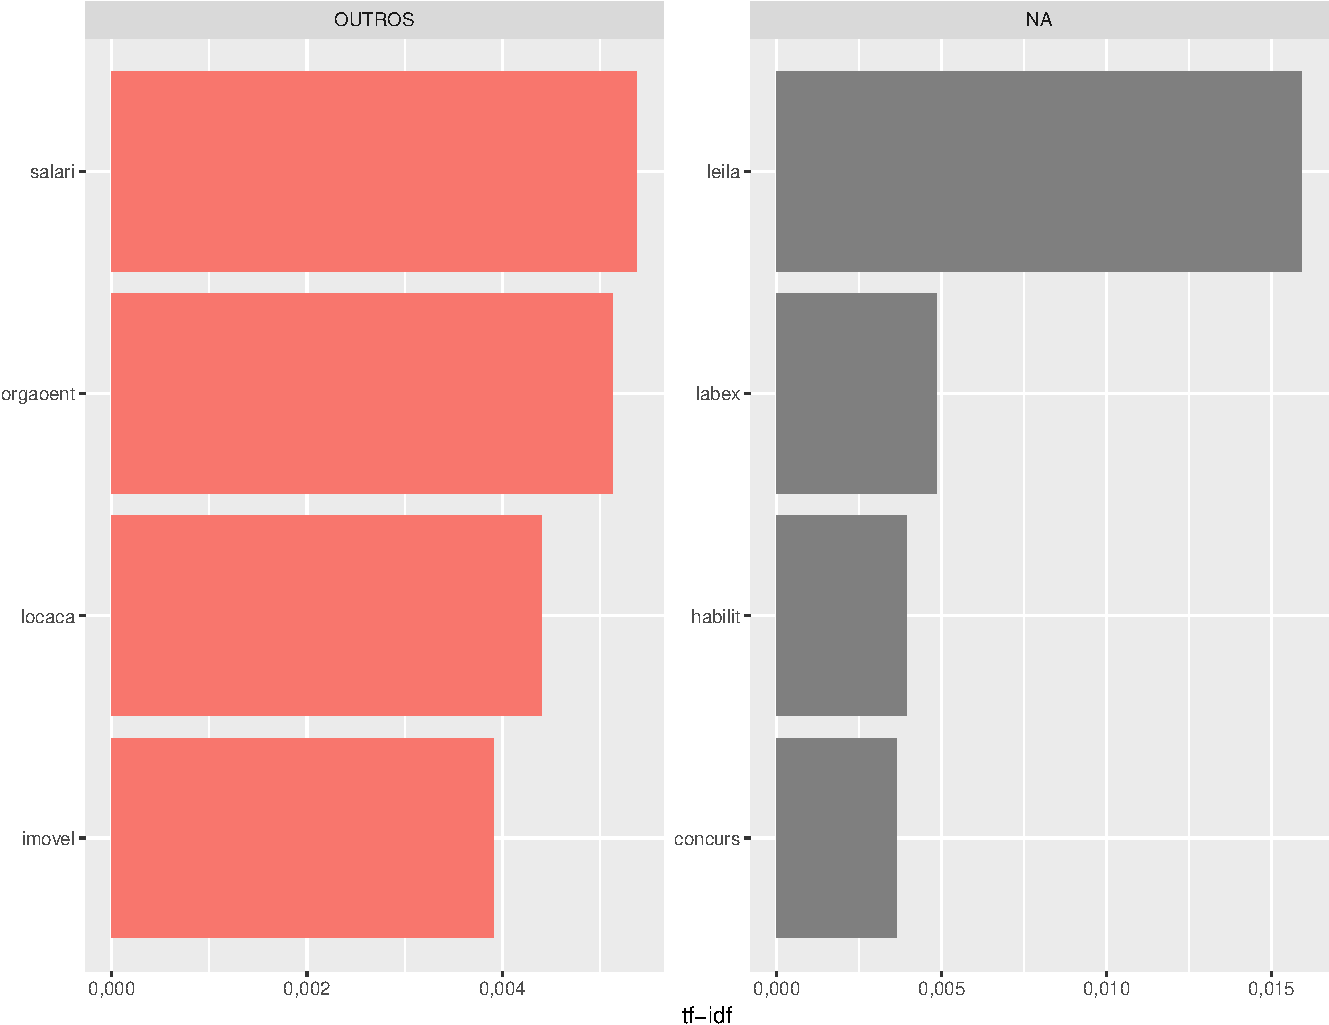
\includegraphics{markdown_v50_files/figure-latex/unnamed-chunk-71-1.pdf}

\begin{Shaded}
\begin{Highlighting}[]
\CommentTok{#dev.off()}
\end{Highlighting}
\end{Shaded}

\hypertarget{figura5-termos-mais-relevantes-por-diretoria-pela-estatistica-tf_idf-apos-stemming-e-sem-stop-words}{%
\subparagraph{\texorpdfstring{Figura5: Termos mais relevantes por
diretoria pela estatística \textbf{tf\_idf}, após \textbf{stemming} e
sem \textbf{stop
words}}{Figura5: Termos mais relevantes por diretoria pela estatística tf\_idf, após stemming e sem stop words}}\label{figura5-termos-mais-relevantes-por-diretoria-pela-estatistica-tf_idf-apos-stemming-e-sem-stop-words}}

Sim, a remoção de \textbf{stop words} não alterou em nada a ordem das 4
palavras mais relevantes de acordo com a estatística.

\begin{Shaded}
\begin{Highlighting}[]
\CommentTok{#diretoria_palavras_noSTOP_noSTOP}
\NormalTok{plot_diretoria_palavras_noSTOP <-}\StringTok{ }\NormalTok{diretoria_palavras_noSTOP }\OperatorTok
\StringTok{  }\KeywordTok{bind_tf_idf}\NormalTok{(palavra, DIRETORIA, n) }\OperatorTok
\StringTok{  }\KeywordTok{arrange}\NormalTok{(}\KeywordTok{desc}\NormalTok{(tf_idf)) }\OperatorTok
\StringTok{  }\KeywordTok{mutate}\NormalTok{(}\DataTypeTok{word =} \KeywordTok{factor}\NormalTok{(palavra, }\DataTypeTok{levels =} \KeywordTok{rev}\NormalTok{(}\KeywordTok{unique}\NormalTok{(palavra)))) }\OperatorTok
\StringTok{  }\KeywordTok{mutate}\NormalTok{(}\DataTypeTok{DIRETORIA =} \KeywordTok{factor}\NormalTok{(DIRETORIA, }\DataTypeTok{levels =} \KeywordTok{c}\NormalTok{(}\StringTok{"DEA"}\NormalTok{,}\StringTok{"DEE"}\NormalTok{,}\StringTok{"OUTROS"}\NormalTok{)))}
\CommentTok{#plot_diretoria_palavras_noSTOP}
\CommentTok{#windows.options(width=10, height=10)}
\CommentTok{#jpeg("03_freq_palavras_dir_nostop.jpeg")}
\NormalTok{plot_diretoria_palavras_noSTOP }\OperatorTok
\StringTok{  }\KeywordTok{group_by}\NormalTok{(DIRETORIA) }\OperatorTok
\StringTok{  }\KeywordTok{top_n}\NormalTok{(}\DecValTok{4}\NormalTok{, tf_idf) }\OperatorTok
\StringTok{  }\KeywordTok{ungroup}\NormalTok{() }\OperatorTok
\StringTok{  }\KeywordTok{mutate}\NormalTok{(}\DataTypeTok{palavra =} \KeywordTok{reorder}\NormalTok{(palavra, tf_idf)) }\OperatorTok
\StringTok{  }\KeywordTok{ggplot}\NormalTok{(}\KeywordTok{aes}\NormalTok{(palavra, tf_idf, }\DataTypeTok{fill =}\NormalTok{ DIRETORIA)) }\OperatorTok{+}
\StringTok{  }\KeywordTok{geom_col}\NormalTok{(}\DataTypeTok{show.legend =} \OtherTok{FALSE}\NormalTok{) }\OperatorTok{+}
\StringTok{  }\KeywordTok{labs}\NormalTok{(}\DataTypeTok{x =} \OtherTok{NULL}\NormalTok{, }\DataTypeTok{y =} \StringTok{"tf-idf"}\NormalTok{) }\OperatorTok{+}
\StringTok{  }\KeywordTok{facet_wrap}\NormalTok{(}\OperatorTok{~}\NormalTok{DIRETORIA, }\DataTypeTok{ncol =} \DecValTok{2}\NormalTok{, }\DataTypeTok{scales =} \StringTok{"free"}\NormalTok{) }\OperatorTok{+}
\StringTok{  }\KeywordTok{coord_flip}\NormalTok{() }\OperatorTok{+}\StringTok{ }
\StringTok{  }\KeywordTok{scale_y_continuous}\NormalTok{(}\DataTypeTok{labels=}\NormalTok{gcomma)}
\end{Highlighting}
\end{Shaded}

\begin{verbatim}
## Warning: Factor `DIRETORIA` contains implicit NA, consider using
## `forcats::fct_explicit_na`
\end{verbatim}

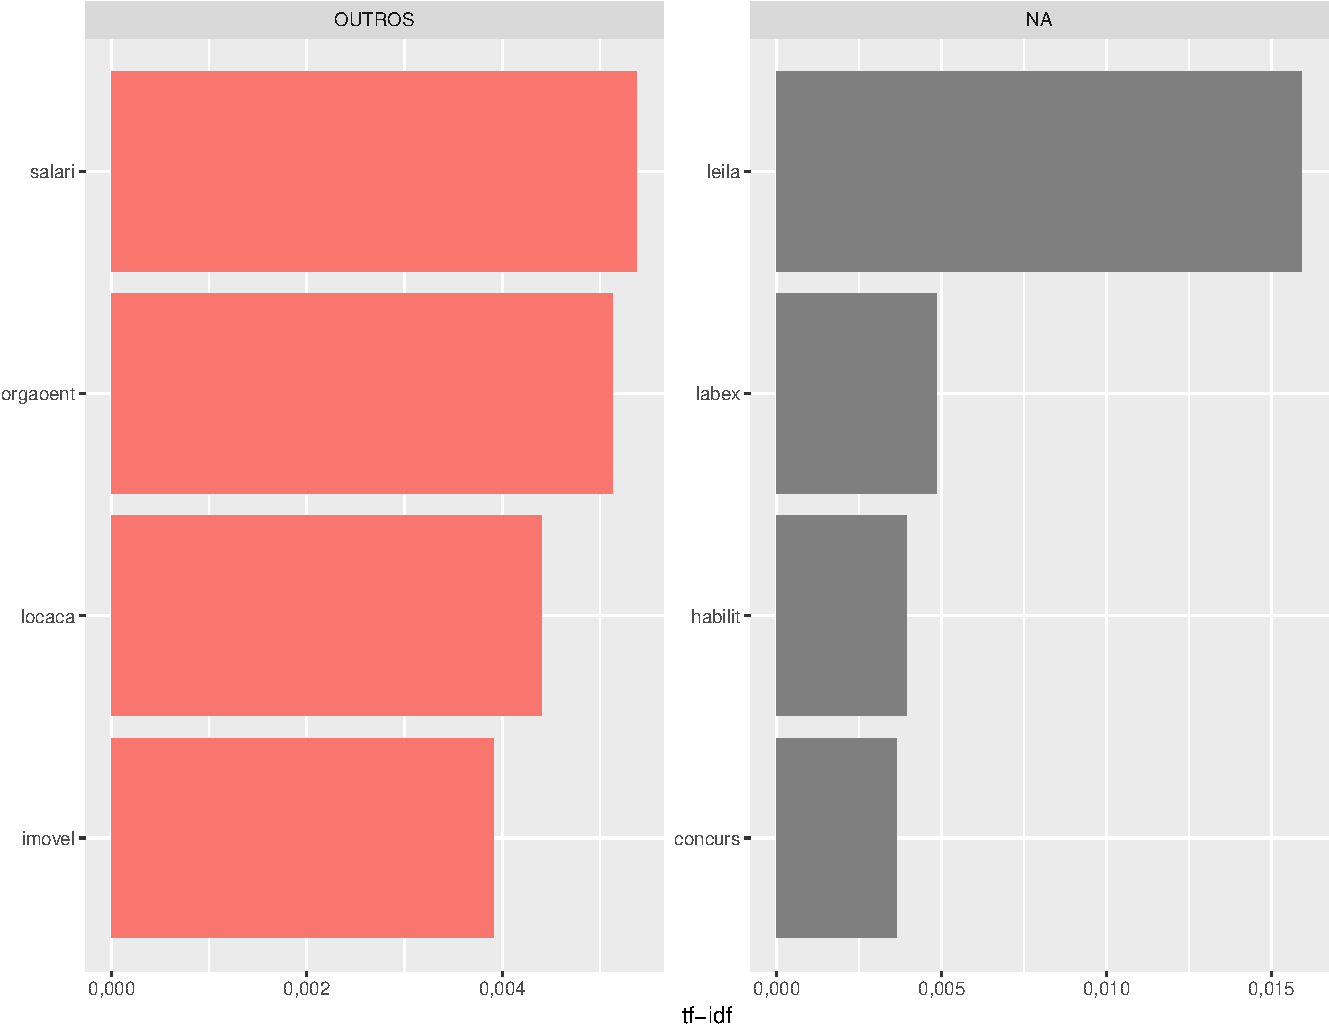
\includegraphics{markdown_v50_files/figure-latex/03_freq_palavras_dir_nostop-1.pdf}

\begin{Shaded}
\begin{Highlighting}[]
\CommentTok{#dev.off()}
\end{Highlighting}
\end{Shaded}

\hypertarget{wordcloud2---dee}{%
\subparagraph{Wordcloud2 - DEE}\label{wordcloud2---dee}}

\begin{Shaded}
\begin{Highlighting}[]
\NormalTok{set.seed(6423)}
\NormalTok{plot_diretoria_palavras_noSTOP %>%}
\NormalTok{  filter(DIRETORIA == }\StringTok{"DEE"}\NormalTok{) %>%}
\NormalTok{  select(word = palavra, freq = tf_idf) %>%}
\NormalTok{  mutate(word = as.factor(word)) %>%}
  \CommentTok{#top_n(150, freq) %>%}
\NormalTok{  as.data.frame() %>%}
\NormalTok{  wordcloud2(shuffle = TRUE, color = }\StringTok{"random-dark"}\NormalTok{, shape = }\StringTok{"circle"}\NormalTok{, size = 1.10)}
\end{Highlighting}
\end{Shaded}

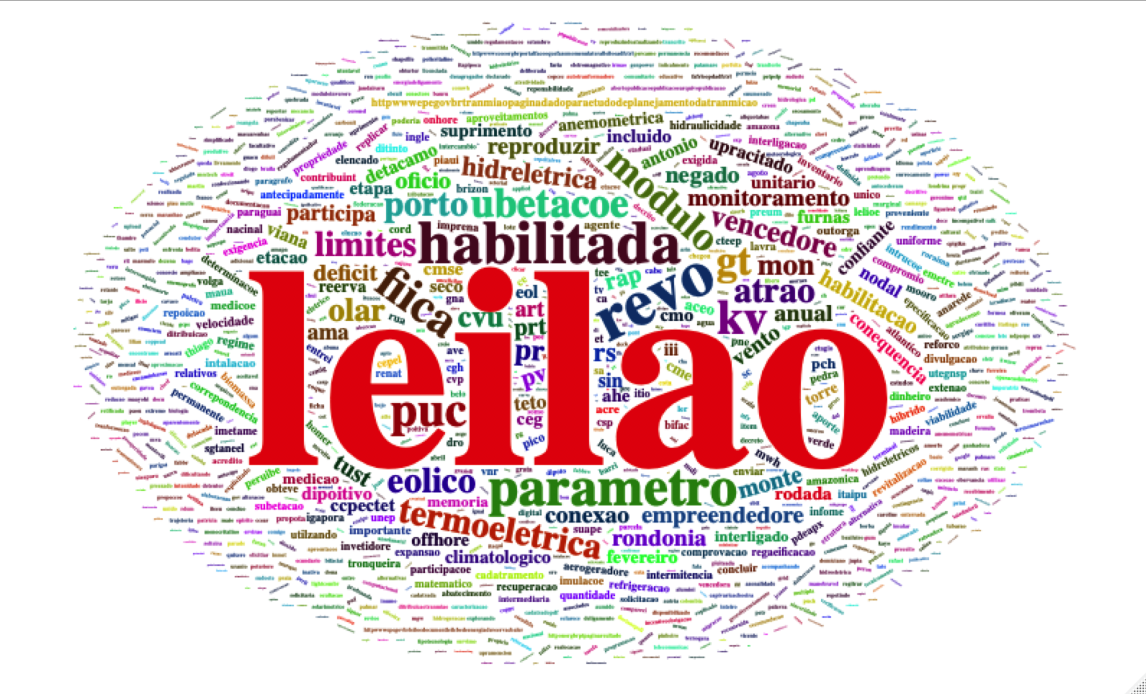
\includegraphics[width=400px]{/Users/ewersonpimenta/Desktop/ESIC_TCC/TCC_v2.1/RMARKDOWN/IMAGENS/WORDCLOUDS/01.ONEGRAM_wordcloud2_DEE01}

\hypertarget{wordcloud2---dea}{%
\subparagraph{Wordcloud2 - DEA}\label{wordcloud2---dea}}

\begin{Shaded}
\begin{Highlighting}[]
\NormalTok{set.seed(6423)}
\NormalTok{plot_diretoria_palavras_noSTOP %>%}
\NormalTok{  filter(DIRETORIA == }\StringTok{"DEA"}\NormalTok{) %>%}
\NormalTok{  select(word = palavra, freq = tf_idf) %>%}
\NormalTok{  mutate(word = as.factor(word)) %>%}
  \CommentTok{#top_n(150, freq) %>%}
\NormalTok{  as.data.frame() %>%}
\NormalTok{  wordcloud2(shuffle = TRUE, color = }\StringTok{"random-dark"}\NormalTok{, shape = }\StringTok{"circle"}\NormalTok{, size = .25)}
\end{Highlighting}
\end{Shaded}

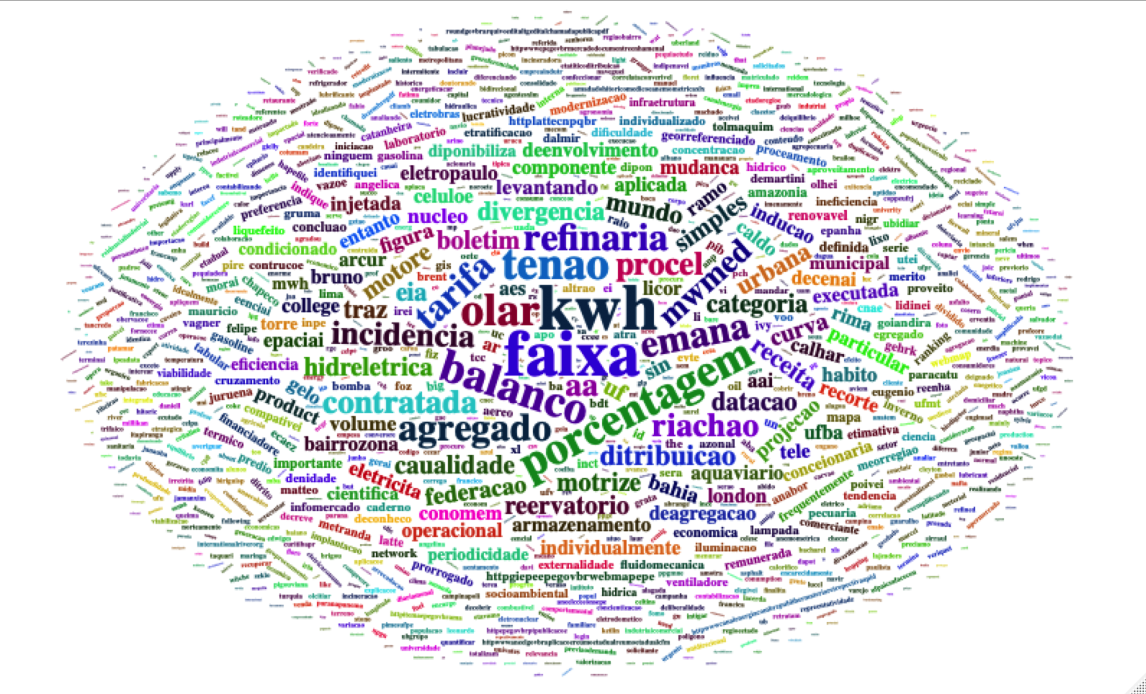
\includegraphics[width=400px]{/Users/ewersonpimenta/Desktop/ESIC_TCC/TCC_v2.1/RMARKDOWN/IMAGENS/WORDCLOUDS/01.ONEGRAM_wordcloud2_DEA01}

\hypertarget{wordcloud2---outros}{%
\subparagraph{Wordcloud2 - OUTROS}\label{wordcloud2---outros}}

\begin{Shaded}
\begin{Highlighting}[]
\NormalTok{set.seed(6423)}
\NormalTok{plot_diretoria_palavras_noSTOP %>%}
\NormalTok{  filter(DIRETORIA == }\StringTok{"OUTROS"}\NormalTok{) %>%}
\NormalTok{  select(word = palavra, freq = tf_idf) %>%}
\NormalTok{  mutate(word = as.factor(word)) %>%}
  \CommentTok{#top_n(150, freq) %>%}
\NormalTok{  as.data.frame() %>%}
\NormalTok{  wordcloud2(shuffle = TRUE, color = }\StringTok{"random-dark"}\NormalTok{, shape = }\StringTok{"circle"}\NormalTok{, size = 0.35)}
\end{Highlighting}
\end{Shaded}

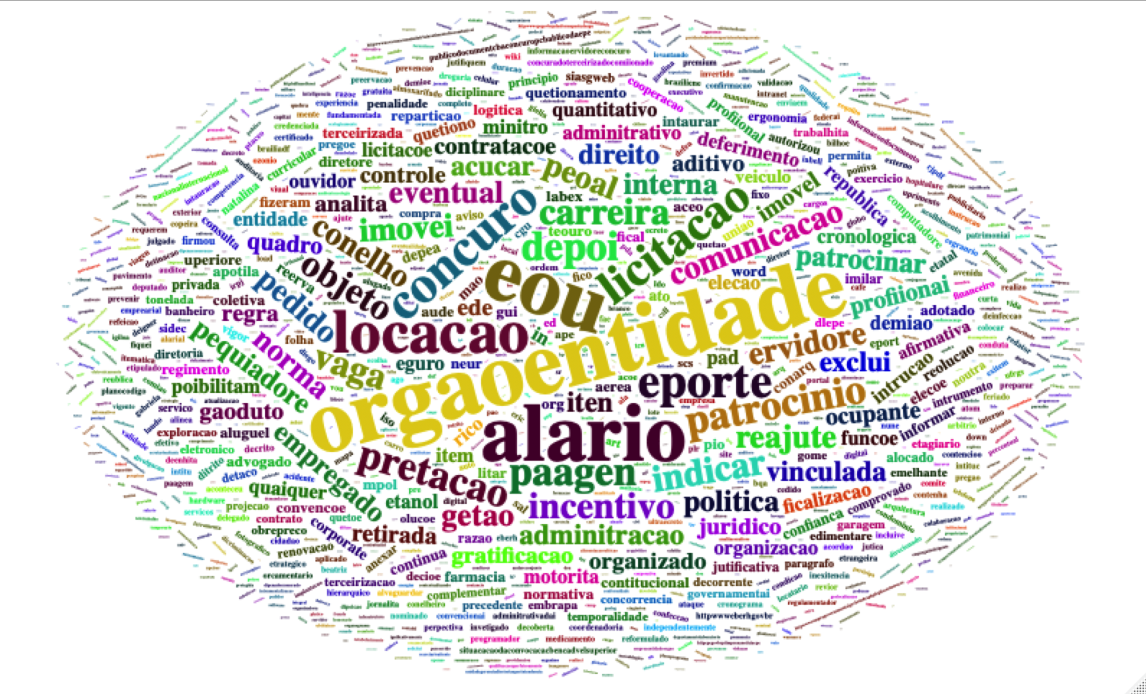
\includegraphics[width=400px]{/Users/ewersonpimenta/Desktop/ESIC_TCC/TCC_v2.1/RMARKDOWN/IMAGENS/WORDCLOUDS/01.ONEGRAM_wordcloud2_OUTROS01}

\hypertarget{comparacao-de-frequencias-dois-a-dois-sem-stopwords-e-com-stemming}{%
\paragraph{Comparação de frequências dois a dois (sem stopwords e com
stemming)}\label{comparacao-de-frequencias-dois-a-dois-sem-stopwords-e-com-stemming}}

Vamos agora comparar a frequência de palavras entre diretorias. Antes
disso, vamos criar documentos de texto no formato tidy separadamente
para cada uma das 3 cateorias: \emph{DEA}, \emph{DEE} e \emph{OUTROS}.

\begin{Shaded}
\begin{Highlighting}[]
\KeywordTok{\{}\NormalTok{r child = '032_textminingpart2.Rmd'}\KeywordTok{\}}
\end{Highlighting}
\end{Shaded}

\hypertarget{modelagem---aplicacao-e-resultados}{%
\section{MODELAGEM - APLICAÇÃO E
RESULTADOS}\label{modelagem---aplicacao-e-resultados}}

\hypertarget{preparacao-e-particao-de-dados}{%
\subsection{Preparação e partição de
dados}\label{preparacao-e-particao-de-dados}}

Recapitulando, chegamos portanto, a uma base de dados donde foram
aplicadas 2 diferentes técnicas de \textbf{stemming}, também a remoção
de \textbf{stopwords} e fazendo uso da estatística \textbf{tf\_idf} a
fim de ressaltar os termos mais relevantes de cada documento de texto.

Vamos, portanto, contar o número de termos únicos dentro de cada
diretoria.

\hypertarget{tabela11-numero-de-termos-unicos-por-diretoria}{%
\subparagraph{Tabela11: Número de termos únicos por
diretoria}\label{tabela11-numero-de-termos-unicos-por-diretoria}}

\begin{Shaded}
\begin{Highlighting}[]
\NormalTok{key_DIR =}\StringTok{ }\NormalTok{plot_diretoria_palavras_noSTOP }\OperatorTok
\StringTok{  }\KeywordTok{group_by}\NormalTok{(DIRETORIA) }\OperatorTok
\StringTok{  }\KeywordTok{count}\NormalTok{(DIRETORIA)}
\end{Highlighting}
\end{Shaded}

\begin{verbatim}
## Warning: Factor `DIRETORIA` contains implicit NA, consider using
## `forcats::fct_explicit_na`

## Warning: Factor `DIRETORIA` contains implicit NA, consider using
## `forcats::fct_explicit_na`

## Warning: Factor `DIRETORIA` contains implicit NA, consider using
## `forcats::fct_explicit_na`
\end{verbatim}

\begin{Shaded}
\begin{Highlighting}[]
\NormalTok{ key_DIR }\OperatorTok
\StringTok{   }\KeywordTok{kable}\NormalTok{(}\StringTok{"latex"}\NormalTok{, }\DataTypeTok{caption =} \StringTok{"Número de termos por diretoria"}\NormalTok{, }
        \DataTypeTok{booktabs =}\NormalTok{ T, }\DataTypeTok{format.args =} \KeywordTok{list}\NormalTok{(}\DataTypeTok{decimal.mark =} \StringTok{','}\NormalTok{, }\DataTypeTok{big.mark =} \StringTok{"."}\NormalTok{)) }\OperatorTok
\StringTok{  }\KeywordTok{kable_styling}\NormalTok{(}\DataTypeTok{latex_options =} \KeywordTok{c}\NormalTok{(}\StringTok{"striped"}\NormalTok{, }\StringTok{"hold_position"}\NormalTok{))}
\end{Highlighting}
\end{Shaded}

\begin{table}[!h]

\caption{\label{tab:unnamed-chunk-75}Número de termos por diretoria}
\centering
\begin{tabular}{lr}
\toprule
DIRETORIA & n\\
\midrule
\rowcolor{gray!6}  OUTROS & 1.400\\
NA & 3.728\\
\bottomrule
\end{tabular}
\end{table}

Vamos, agora, selecionar as \(n=250\) palavras mais importantes de cada
uma das 4 diretorias e da categoria `OUTROS'. Para isso vamos, primeiro,
separar os documentos em 3 documentos distintos, um para cada diretoria.

\begin{Shaded}
\begin{Highlighting}[]
\NormalTok{n=}\DecValTok{25}
\CommentTok{#n=500}
\CommentTok{#n=500}

\NormalTok{termos_dir_DEE =}\StringTok{ }
\NormalTok{plot_diretoria_palavras_noSTOP }\OperatorTok
\KeywordTok{filter}\NormalTok{(DIRETORIA }\OperatorTok{==}\StringTok{ "DEE"}\NormalTok{)}
\NormalTok{termos_DEE =}\StringTok{ }\NormalTok{termos_dir_DEE }\OperatorTok
\StringTok{  }\KeywordTok{top_n}\NormalTok{(n, tf_idf)}

\NormalTok{termos_dir_DEA =}\StringTok{ }
\NormalTok{plot_diretoria_palavras_noSTOP }\OperatorTok
\KeywordTok{filter}\NormalTok{(DIRETORIA }\OperatorTok{==}\StringTok{ "DEA"}\NormalTok{)}
\NormalTok{termos_DEA =}\StringTok{ }\NormalTok{termos_dir_DEA }\OperatorTok
\StringTok{  }\KeywordTok{top_n}\NormalTok{(n, tf_idf)}

\NormalTok{termos_dir_OUTROS =}\StringTok{ }
\NormalTok{plot_diretoria_palavras_noSTOP }\OperatorTok
\KeywordTok{filter}\NormalTok{(DIRETORIA }\OperatorTok{==}\StringTok{ "OUTROS"}\NormalTok{)}
\NormalTok{termos_OUTROS =}\StringTok{ }\NormalTok{termos_dir_OUTROS }\OperatorTok
\StringTok{  }\KeywordTok{top_n}\NormalTok{(n}\OperatorTok{*}\DecValTok{3}\NormalTok{, tf_idf)}

\NormalTok{termos_dir =}\StringTok{ }\KeywordTok{bind_rows}\NormalTok{(}\KeywordTok{mutate}\NormalTok{(termos_DEE, }\DataTypeTok{DIRETORIA =} \StringTok{"DEE"}\NormalTok{),}
                         \KeywordTok{mutate}\NormalTok{(termos_DEA, }\DataTypeTok{DIRETORIA =} \StringTok{"DEA"}\NormalTok{),}
                         \KeywordTok{mutate}\NormalTok{(termos_OUTROS, }\DataTypeTok{DIRETORIA =} \StringTok{"OUTROS"}\NormalTok{)) }\OperatorTok
\StringTok{  }\KeywordTok{select}\NormalTok{(palavra) }\OperatorTok
\StringTok{  }\KeywordTok{unique}\NormalTok{()}
\end{Highlighting}
\end{Shaded}

\begin{Shaded}
\begin{Highlighting}[]
\NormalTok{gg <-}\StringTok{ }\NormalTok{termos_dir}\OperatorTok{$}\NormalTok{palavra}
\NormalTok{gg <-}\StringTok{ }\KeywordTok{unique}\NormalTok{(gg)}
\NormalTok{fe <-}\StringTok{ }\KeywordTok{matrix}\NormalTok{(}\DataTypeTok{data =} \DecValTok{0}\NormalTok{, }\DataTypeTok{nrow =} \KeywordTok{length}\NormalTok{(DB}\OperatorTok{$}\NormalTok{PEDIDO1), }\DataTypeTok{ncol =} \KeywordTok{length}\NormalTok{(gg))}
\NormalTok{fe <-}\StringTok{ }\KeywordTok{data.frame}\NormalTok{(fe); }\KeywordTok{colnames}\NormalTok{(fe) <-}\StringTok{ }\NormalTok{gg}
\NormalTok{i=j=}\DecValTok{0}
\ControlFlowTok{for}\NormalTok{(i }\ControlFlowTok{in} \DecValTok{1}\OperatorTok{:}\KeywordTok{length}\NormalTok{(DB}\OperatorTok{$}\NormalTok{Protocolo))\{}
        \ControlFlowTok{for}\NormalTok{(j }\ControlFlowTok{in} \DecValTok{1}\OperatorTok{:}\KeywordTok{length}\NormalTok{(gg))\{}
\NormalTok{                g <-}\StringTok{ }\KeywordTok{grepl}\NormalTok{(gg[j], DB}\OperatorTok{$}\NormalTok{PEDIDO1[i])}
                \ControlFlowTok{if}\NormalTok{(g }\OperatorTok{==}\StringTok{ }\OtherTok{TRUE}\NormalTok{)\{}
\NormalTok{                        fe[i, j] <-}\StringTok{ }\DecValTok{1}        
\NormalTok{                \}}
\NormalTok{        \}}
\NormalTok{\}}

\CommentTok{#sum(rowSums(fe))}
\KeywordTok{dim}\NormalTok{(fe)}
\end{Highlighting}
\end{Shaded}

\begin{verbatim}
## [1] 624  99
\end{verbatim}

\begin{Shaded}
\begin{Highlighting}[]
\CommentTok{#colSums(fe)}
\KeywordTok{cat}\NormalTok{(}\KeywordTok{paste0}\NormalTok{(}\StringTok{"Existem "}\NormalTok{, }\KeywordTok{dim}\NormalTok{(fe)[}\DecValTok{2}\NormalTok{], }\StringTok{" termos/palavras-chaves únicas na matriz em questão."}\NormalTok{))}
\end{Highlighting}
\end{Shaded}

\begin{verbatim}
## Existem 99 termos/palavras-chaves únicas na matriz em questão.
\end{verbatim}

\begin{Shaded}
\begin{Highlighting}[]
\NormalTok{NumTermos =}\StringTok{ }\KeywordTok{as_tibble}\NormalTok{(}\KeywordTok{rbind}\NormalTok{(}\KeywordTok{apply}\NormalTok{(fe,}\DecValTok{2}\NormalTok{,sum)))}
\NormalTok{NumTermos =}\StringTok{ }\KeywordTok{gather}\NormalTok{(NumTermos, }\DataTypeTok{key =} \StringTok{"termo"}\NormalTok{, }\DataTypeTok{value =} \StringTok{"Num_Pedidos"}\NormalTok{)}
\NormalTok{NumTermos =}\StringTok{ }\NormalTok{NumTermos[}\KeywordTok{order}\NormalTok{(NumTermos}\OperatorTok{$}\NormalTok{Num_Pedidos, }\DataTypeTok{decreasing =} \OtherTok{TRUE}\NormalTok{), ]}
\CommentTok{#View(colSums(fe))}
\CommentTok{#View(colnames(fe))}
\end{Highlighting}
\end{Shaded}

Vamos excluir alguns termos com pouca frequência (abaixo de 8) (abaixo
do terceiro quartil)

\begin{Shaded}
\begin{Highlighting}[]
\KeywordTok{summary}\NormalTok{(}\KeywordTok{colSums}\NormalTok{(fe))}
\end{Highlighting}
\end{Shaded}

\begin{verbatim}
##    Min. 1st Qu.  Median    Mean 3rd Qu.    Max. 
##    1.00    3.00    5.00   11.77    9.00  310.00
\end{verbatim}

\begin{Shaded}
\begin{Highlighting}[]
 \CommentTok{#removing unecessary terms}
\NormalTok{    exclui_termos <-}\StringTok{ }\KeywordTok{as.character}\NormalTok{(}\KeywordTok{c}\NormalTok{())}
     \KeywordTok{cbind}\NormalTok{(}\DataTypeTok{Termos =} \KeywordTok{colnames}\NormalTok{(fe), }\DataTypeTok{Freq_Termos =} \KeywordTok{colSums}\NormalTok{(fe))}
\end{Highlighting}
\end{Shaded}

\begin{verbatim}
##              Termos         Freq_Termos
## salari       "salari"       "10"       
## orgaoent     "orgaoent"     "8"        
## locaca       "locaca"       "10"       
## imovel       "imovel"       "4"        
## pessoal      "pessoal"      "9"        
## carr         "carr"         "6"        
## prestaca     "prestaca"     "8"        
## empreg       "empreg"       "18"       
## it           "it"           "310"      
## gasodut      "gasodut"      "7"        
## reajust      "reajust"      "3"        
## func         "func"         "41"       
## control      "control"      "5"        
## gratificaca  "gratificaca"  "3"        
## seleca       "seleca"       "3"        
## anal         "anal"         "60"       
## audi         "audi"         "7"        
## contrataco   "contrataco"   "5"        
## direit       "direit"       "6"        
## jurid        "jurid"        "5"        
## licitaco     "licitaco"     "4"        
## loc          "loc"          "45"       
## ocup         "ocup"         "8"        
## ouvid        "ouvid"        "3"        
## sed          "sed"          "11"       
## segur        "segur"        "7"        
## concurs      "concurs"      "24"       
## esport       "esport"       "4"        
## licitaca     "licitaca"     "9"        
## quadr        "quadr"        "14"       
## vag          "vag"          "12"       
## veicul       "veicul"       "8"        
## adit         "adit"         "6"        
## cronolog     "cronolog"     "2"        
## demissa      "demissa"      "4"        
## desp         "desp"         "11"       
## exclus       "exclus"       "3"        
## fiscalizaca  "fiscalizaca"  "2"        
## instruca     "instruca"     "3"        
## organizaca   "organizaca"   "3"        
## quantit      "quantit"      "4"        
## regr         "regr"         "5"        
## retir        "retir"        "3"        
## terceir      "terceir"      "9"        
## terceirizaca "terceirizaca" "3"        
## patrocini    "patrocini"    "4"        
## projeca      "projeca"      "10"       
## administr    "administr"    "28"       
## prec         "prec"         "91"       
## objet        "objet"        "9"        
## aluguel      "aluguel"      "2"        
## conarq       "conarq"       "1"        
## confianc     "confianc"     "2"        
## estagia      "estagia"      "2"        
## etanol       "etanol"       "3"        
## funco        "funco"        "5"        
## ministr      "ministr"      "31"       
## pad          "pad"          "13"       
## quaisqu      "quaisqu"      "4"        
## visual       "visual"       "4"        
## pass         "pass"         "17"       
## aloc         "aloc"         "6"        
## firm         "firm"         "19"       
## fix          "fix"          "8"        
## incen        "incen"        "6"        
## priv         "priv"         "7"        
## simil        "simil"        "9"        
## gesta        "gesta"        "16"       
## acuc         "acuc"         "3"        
## comunicaca   "comunicaca"   "7"        
## fiscal       "fiscal"       "9"        
## parec        "parec"        "15"       
## apostil      "apostil"      "4"        
## aven         "aven"         "2"        
## cole         "cole"         "13"       
## complement   "complement"   "3"        
## conform      "conform"      "3"        
## constituc    "constituc"    "4"        
## continu      "continu"      "5"        
## convenco     "convenco"     "2"        
## corporat     "corporat"     "2"        
## curricul     "curricul"     "3"        
## desinfecca   "desinfecca"   "2"        
## empresar     "empresar"     "2"        
## ergonom      "ergonom"      "2"        
## exploraca    "exploraca"    "3"        
## farmac       "farmac"       "1"        
## folh         "folh"         "3"        
## instaur      "instaur"      "4"        
## logis        "logis"        "2"        
## mao          "mao"          "4"        
## natalin      "natalin"      "1"        
## salar        "salar"        "10"       
## sediment     "sediment"     "3"        
## seleco       "seleco"       "1"        
## temporal     "temporal"     "1"        
## tesour       "tesour"       "3"        
## vig          "vig"          "12"       
## word         "word"         "4"
\end{verbatim}

\begin{Shaded}
\begin{Highlighting}[]
\NormalTok{    z=}\DecValTok{0}
    \ControlFlowTok{for}\NormalTok{ (k }\ControlFlowTok{in} \DecValTok{1}\OperatorTok{:}\KeywordTok{dim}\NormalTok{(fe)[}\DecValTok{2}\NormalTok{]) \{}
      \ControlFlowTok{if}\NormalTok{ (}\KeywordTok{colSums}\NormalTok{(fe)[k] }\OperatorTok{<=}\StringTok{ }\DecValTok{7}\NormalTok{) \{}
\NormalTok{        exclui_termos[z] <-}\StringTok{ }\KeywordTok{colnames}\NormalTok{(fe)[k]}
\NormalTok{        z =}\StringTok{ }\NormalTok{z}\OperatorTok{+}\DecValTok{1}
\NormalTok{      \}}
\NormalTok{    \}}
    
      \CommentTok{#length(exclui_termos) # [1] 409 [1] 2118}
    
    \KeywordTok{cat}\NormalTok{(}\KeywordTok{paste0}\NormalTok{(}\StringTok{"Existem "}\NormalTok{, }\KeywordTok{length}\NormalTok{(exclui_termos), }\StringTok{" termos com freq. menor ou igual a 7. Logo, se removermos estes o número de variáveis (termos) resultante será igual a "}\NormalTok{, }\KeywordTok{dim}\NormalTok{(fe)[}\DecValTok{2}\NormalTok{] }\OperatorTok{-}\StringTok{ }\KeywordTok{length}\NormalTok{(exclui_termos), }\StringTok{" termos únicos."}\NormalTok{))}
\end{Highlighting}
\end{Shaded}

\begin{verbatim}
## Existem 63 termos com freq. menor ou igual a 7. Logo, se removermos estes o número de variáveis (termos) resultante será igual a 36 termos únicos.
\end{verbatim}

\begin{Shaded}
\begin{Highlighting}[]
\NormalTok{    fe <-}\StringTok{ }\NormalTok{fe }\OperatorTok\StringTok{ }\KeywordTok{select}\NormalTok{(}\OperatorTok{-}\NormalTok{exclui_termos)}
\end{Highlighting}
\end{Shaded}

\begin{Shaded}
\begin{Highlighting}[]
\KeywordTok{cat}\NormalTok{(}\KeywordTok{paste0}\NormalTok{(}\StringTok{"Existem, agora, "}\NormalTok{, }\KeywordTok{dim}\NormalTok{(fe)[}\DecValTok{2}\NormalTok{], }\StringTok{" termos/palavras-chaves únicas."}\NormalTok{))}
\end{Highlighting}
\end{Shaded}

\begin{verbatim}
## Existem, agora, 36 termos/palavras-chaves únicas.
\end{verbatim}

\hypertarget{criterio-de-escolha-dos-termos-se-a-frequencia-for-maior-ou-igual-a-10}{%
\subsubsection{Critério de escolha dos termos, se a frequência for maior
ou igual a
10}\label{criterio-de-escolha-dos-termos-se-a-frequencia-for-maior-ou-igual-a-10}}

IMPLEMENTAR

\begin{Shaded}
\begin{Highlighting}[]
\NormalTok{highchart() %>%}
\NormalTok{  hc_add_series(data = NumTermos$Num_Pedidos, }
\NormalTok{                type = }\StringTok{"bar"}\NormalTok{,}
\NormalTok{                name = }\StringTok{"# de pedidos"}\NormalTok{,}
\NormalTok{                showInLegend = FALSE,}
\NormalTok{                tooltip = list(valueDecimals = 0, valuePrefix = }\StringTok{""}\NormalTok{, valueSuffix = }\StringTok{""}\NormalTok{), color=}\StringTok{"blue"}\NormalTok{) %>%}
\NormalTok{  hc_yAxis(title = list(text = }\StringTok{"Quantitativo de pedidos"}\NormalTok{), }
\NormalTok{           allowDecimals = TRUE, max = (max(NumTermos$Num_Pedidos)+103),}
\NormalTok{           labels = list(format = }\StringTok{"\{value\}"}\NormalTok{)) %>%}
\NormalTok{  hc_xAxis(title = list(text = }\StringTok{"Termo"}\NormalTok{),}
\NormalTok{           categories = NumTermos$termo,}
\NormalTok{           tickmarkPlacement = }\StringTok{"on"}\NormalTok{,}
\NormalTok{           opposite = FALSE) %>%}
\NormalTok{  hc_title(text = }\StringTok{"Quantitativo de pedidos por termo (sem exclusividade)"}\NormalTok{,}
\NormalTok{           style = list(fontWeight = }\StringTok{"bold"}\NormalTok{)) %>% }
\NormalTok{  hc_subtitle(text = paste(}\StringTok{""}\NormalTok{)) %>%}
\NormalTok{      hc_tooltip(valueDecimals = 2,}
\NormalTok{                 pointFormat = }\StringTok{"\{point.y\} pedidos"}\NormalTok{)%>%}
                 \CommentTok{#pointFormat = "Variável: \{point.x\} <br> Missing: \{point.y\}") }
\NormalTok{      hc_credits(enabled = TRUE, }
                 \FunctionTok{text = "Fonte:}\AttributeTok{ CGU, e-SIC (2019). Elaboração: Ewerson Pimenta.",}
\NormalTok{                 style = list(fontSize = }\StringTok{"10px"}\NormalTok{)) %>%}
\NormalTok{  hc_exporting(enabled = TRUE, filename = }\StringTok{"F3-filmes-genero-Pimenta"}\NormalTok{)}
\end{Highlighting}
\end{Shaded}

\begin{Shaded}
\begin{Highlighting}[]
\NormalTok{db_modelo0 =}\StringTok{ }\KeywordTok{as_tibble}\NormalTok{(}\KeywordTok{cbind}\NormalTok{(}\KeywordTok{select}\NormalTok{(DB,Protocolo, DATA_REGISTRO, DIRETORIAS, DIRETORIA),fe))}
\NormalTok{db_modelo =}\StringTok{ }\KeywordTok{as_tibble}\NormalTok{(}\KeywordTok{cbind}\NormalTok{(}\KeywordTok{select}\NormalTok{(DB,DIRETORIA),fe))}
\end{Highlighting}
\end{Shaded}

\begin{Shaded}
\begin{Highlighting}[]
\CommentTok{# __Porcentagem de ZEROS por variável__}

\NormalTok{zeros <- (colSums(fe==0)/nrow(fe)*100); var <- names(fe)}
\NormalTok{db_zero <- data.frame(var,zeros); rownames(db_zero) <- NULL}
\NormalTok{db_zero <- db_zero}\KeywordTok{[}\NormalTok{order(db_zero$zeros}\KeywordTok{,}\NormalTok{ decreasing = TRUE)}\KeywordTok{,} \KeywordTok{]}

\NormalTok{hc4_1 <- highchart() %>%}
\NormalTok{  hc_add_series(data = db_zero$zeros, }
\NormalTok{                type = }\StringTok{"bar"}\NormalTok{,}
\NormalTok{                name = }\StringTok{"Porcentagem de zeros"}\NormalTok{,}
\NormalTok{                showInLegend = FALSE,}
\NormalTok{                tooltip = list(valueDecimals = 2, valuePrefix = }\StringTok{""}\NormalTok{, valueSuffix = }\StringTok{" %"}\NormalTok{), color=}\StringTok{"pink"}\NormalTok{) %>%}
\NormalTok{  hc_yAxis(title = list(text = }\StringTok{"Porcentagem de zero"}\NormalTok{), }
\NormalTok{           allowDecimals = TRUE, max = 100,}
\NormalTok{           labels = list(format = }\StringTok{"\{value\}%"}\NormalTok{)) %>%}
\NormalTok{  hc_xAxis(categories = db_zero$var,}
\NormalTok{           tickmarkPlacement = }\StringTok{"on"}\NormalTok{,}
\NormalTok{           opposite = FALSE) %>%}
\NormalTok{  hc_title(text = }\StringTok{"Porcentagem de zeros por variável"}\NormalTok{,}
\NormalTok{           style = list(fontWeight = }\StringTok{"bold"}\NormalTok{)) %>% }
\NormalTok{  hc_subtitle(text = paste(}\StringTok{""}\NormalTok{)) %>%}
\NormalTok{      hc_tooltip(valueDecimals = 2,}
                 \FunctionTok{pointFormat = "Zeros:}\AttributeTok{ }\KeywordTok{\{}\NormalTok{point.y}\KeywordTok{\}}\StringTok{")%>%}
\StringTok{                 #pointFormat = "}\ErrorTok{Variável: \{point.x\} <br> Missing: \{point.y\}") }
\NormalTok{      hc_credits(enabled = TRUE, }
                 \FunctionTok{text = "Fonte:}\AttributeTok{ IMDB/KAGGLE. Elaboração: Ewerson Pimenta.",}
\NormalTok{                 style = list(fontSize = }\StringTok{"10px"}\NormalTok{)) %>%}
\NormalTok{  hc_exporting(enabled = TRUE, filename = }\StringTok{"Fig00-Pimenta"}\NormalTok{)}
\CommentTok{#hc <- hc %>% }
\CommentTok{#  hc_add_theme(hc_theme_darkunica())}
\NormalTok{hc4_1; remove(hc4_1, var, zeros)}
\end{Highlighting}
\end{Shaded}

\hypertarget{modelos-de-classificacao}{%
\subsection{Modelos de classificação}\label{modelos-de-classificacao}}

\hypertarget{particao-dos-dados}{%
\subsubsection{Partição dos dados}\label{particao-dos-dados}}

Particionando a base de dados em Treino e Teste, esses dois (Treino e
Teste) também terão armazenados as diretorias que foram responsaveis por
cada pedido via amostragem probabilística dos dados originais
separadamente das bases de Treino e Teste.

\begin{Shaded}
\begin{Highlighting}[]
\CommentTok{#db_modelo = as_tibble(cbind(select(DB,DIRETORIA),fe))}
\CommentTok{#getwd()}
\CommentTok{#setwd("/Users/ewersonpimenta/Desktop/ESIC_TCC/TCC_v2.1/RMARKDOWN/WEB_APP/")}
\CommentTok{#write.csv(db_modelo0, file = "db_modelo_rf_v21.csv", row.names = FALSE)}
\CommentTok{#db_modelo = read.csv("db_modelo_rf_v10.csv",header = T); dim(db_modelo)}
\CommentTok{#db_modelo = db_modelo %>% select(-r,-venc)}
\CommentTok{#write.csv(db_modelo, file = "db_modelo_rf_v11.csv", row.names = FALSE)}
\end{Highlighting}
\end{Shaded}

Para amostragem aleatória simples

\begin{Shaded}
\begin{Highlighting}[]
\KeywordTok{set.seed}\NormalTok{(}\DecValTok{098798}\NormalTok{) }\CommentTok{# 756446 ou 75452 (OOB_erro: 35,63% ACC: 65,44%) # 2967 (OOB_erro: 34,15% ACC: 64,98%)  # 1743098 (OOB_erro: 34,4% ACC: 67,28%) #V1 098798 (OOB_erro: 23,34% ACC: 70,51%)}
\NormalTok{intrain <-}\StringTok{ }\KeywordTok{createDataPartition}\NormalTok{(}\DataTypeTok{y =}\NormalTok{ db_modelo}\OperatorTok{$}\NormalTok{DIRETORIA, }\DataTypeTok{p =} \FloatTok{0.65}\NormalTok{, }\DataTypeTok{list =} \OtherTok{FALSE}\NormalTok{)}
\NormalTok{training <-}\StringTok{ }\NormalTok{db_modelo[intrain,]}
\NormalTok{testing <-}\StringTok{ }\NormalTok{db_modelo[}\OperatorTok{-}\NormalTok{intrain,]}
\end{Highlighting}
\end{Shaded}

\hypertarget{modelagem-1---random-forest-rf}{%
\subsubsection{Modelagem 1 - Random Forest
(RF)}\label{modelagem-1---random-forest-rf}}

\hypertarget{random-forest-rf---metodologia}{%
\paragraph{Random Forest (RF) -
Metodologia}\label{random-forest-rf---metodologia}}

\textbf{Descrição} 1. Random Forest foi desenvolvido para agregar
árvores de decisão (modelo de classificação);\\
2. Pode ser usado para modelo de classificação (p/ var. resposta
categórica) ou regressão (no caso de haver variável resposta
contínua);\\
3. Evita \emph{overfitting};\\
4. Permite trabalhar com um largo número de características de um
conjunto de dados;\\
5. Auxilia na seleção de variáveis baseada em um algoritmo que calcula a
importância por variável (assim, tendo conhecimento de quais variáveis
são mais importantes, podemos usar essa informação para outros modelos
de classificação);\\
6. User-friendly: apenas 2 parâmetros livres:

\begin{itemize}
\tightlist
\item
  Trees - ntrees, default 500 (Nº de árvores);
\item
  Variáveis selecionadas via amostragem aleatória candidatas à cada
  ``split'' (quebra da árvore) - mtry, default \(\sqrt{p}\) p/
  classificação e \(\frac{p}{3}\) p/ regressão (p: nº de
  features/variáveis);
\end{itemize}

\textbf{Passo-a-Passo}

É realizado em 3 passos:

\begin{enumerate}
\def\labelenumi{\arabic{enumi}.}
\tightlist
\item
  Desenha as amostras via bootstrap do número de árvores
  \emph{ntrees};\\
\item
  Para cada amostra via bootstrap, cresce o número de árvores
  ``un-puned'' para a escolha da melhor quebra da árvore baseado na
  amostra aleatória do valor predito de mtry a cada nó da árvore;\\
\end{enumerate}

\begin{itemize}
\item
  \begin{enumerate}
  \def\labelenumi{\arabic{enumi}.}
  \setcounter{enumi}{2}
  \tightlist
  \item
    Faz classificação de novos valores usando a maioria de votos p/
    classificação e usa a média p/ regressão baseada nas amostras de
    ntrees.
  \end{enumerate}
\end{itemize}

\hypertarget{random-forest---aplicacao-e-resultados}{%
\paragraph{Random Forest - Aplicação e
Resultados}\label{random-forest---aplicacao-e-resultados}}

Inicialmente utilizaremos o pacote \texttt{randomForest} que implmenta o
algoritmo de Random Forest de Breiman (baseado na clusterização de
Breiman, originalmente codificada em Fortran) que tem por finalidade
classificar e/ou criar regressão. Além disso, pode ser usado em um
modelo não supervisionado para avaliar proximidades entre pontos.

Estamos usando, a partir daqui, a base de treino.

\begin{Shaded}
\begin{Highlighting}[]
\CommentTok{#library(randomForest)}
\CommentTok{#library(rpart)}
\CommentTok{#library(rpart.plot)}
\CommentTok{#rf <- randomForest(proximity = T,ntree = 38,do.trace = T,WR~.,data=training)}
\KeywordTok{set.seed}\NormalTok{(}\DecValTok{9984512}\NormalTok{)}
\CommentTok{# Training with classification tree}
\NormalTok{rf <-}\StringTok{ }\KeywordTok{rpart}\NormalTok{(DIRETORIA }\OperatorTok{~}\StringTok{ }\NormalTok{., }\DataTypeTok{data=}\NormalTok{training, }\DataTypeTok{method=}\StringTok{"class"}\NormalTok{, }\DataTypeTok{xval =} \DecValTok{4}\NormalTok{, )}
\KeywordTok{print}\NormalTok{(rf, }\DataTypeTok{digits =} \DecValTok{3}\NormalTok{)}
\end{Highlighting}
\end{Shaded}

\begin{verbatim}
## n= 408 
## 
## node), split, n, loss, yval, (yprob)
##       * denotes terminal node
## 
##   1) root 408 268 1 (0.3431 0.3358 0.0907 0.2304)  
##     2) administr< 0.5 389 251 1 (0.3548 0.3496 0.0951 0.2005)  
##       4) concurs< 0.5 375 237 1 (0.3680 0.3627 0.0853 0.1840)  
##         8) gesta< 0.5 367 229 1 (0.3760 0.3706 0.0790 0.1744)  
##          16) sed< 0.5 360 223 1 (0.3806 0.3778 0.0778 0.1639)  
##            32) pass< 0.5 352 216 1 (0.3864 0.3807 0.0795 0.1534)  
##              64) func< 0.5 334 202 1 (0.3952 0.3862 0.0778 0.1407)  
##               128) anal>=0.5 31  13 2 (0.2903 0.5806 0.0323 0.0968) *
##               129) anal< 0.5 303 180 1 (0.4059 0.3663 0.0825 0.1452)  
##                 258) it< 0.5 162  89 1 (0.4506 0.3395 0.0741 0.1358) *
##                 259) it>=0.5 141  85 2 (0.3546 0.3972 0.0922 0.1560)  
##                   518) prec>=0.5 21  10 1 (0.5238 0.2381 0.1429 0.0952) *
##                   519) prec< 0.5 120  69 2 (0.3250 0.4250 0.0833 0.1667) *
##              65) func>=0.5 18  11 OUTROS (0.2222 0.2778 0.1111 0.3889) *
##            33) pass>=0.5 8   3 OUTROS (0.1250 0.2500 0.0000 0.6250) *
##          17) sed>=0.5 7   2 OUTROS (0.1429 0.0000 0.1429 0.7143) *
##         9) gesta>=0.5 8   3 OUTROS (0.0000 0.0000 0.3750 0.6250) *
##       5) concurs>=0.5 14   5 OUTROS (0.0000 0.0000 0.3571 0.6429) *
##     3) administr>=0.5 19   3 OUTROS (0.1053 0.0526 0.0000 0.8421) *
\end{verbatim}

\begin{Shaded}
\begin{Highlighting}[]
\KeywordTok{attributes}\NormalTok{(rf)}
\end{Highlighting}
\end{Shaded}

\begin{verbatim}
## $names
##  [1] "frame"               "where"               "call"               
##  [4] "terms"               "cptable"             "method"             
##  [7] "parms"               "control"             "functions"          
## [10] "numresp"             "splits"              "variable.importance"
## [13] "y"                   "ordered"            
## 
## $xlevels
## named list()
## 
## $ylevels
## [1] "1"      "2"      "5"      "OUTROS"
## 
## $class
## [1] "rpart"
\end{verbatim}

\begin{Shaded}
\begin{Highlighting}[]
\KeywordTok{plot}\NormalTok{(rf)}
\KeywordTok{text}\NormalTok{(rf, }\DataTypeTok{use.n =} \OtherTok{TRUE}\NormalTok{)}
\end{Highlighting}
\end{Shaded}

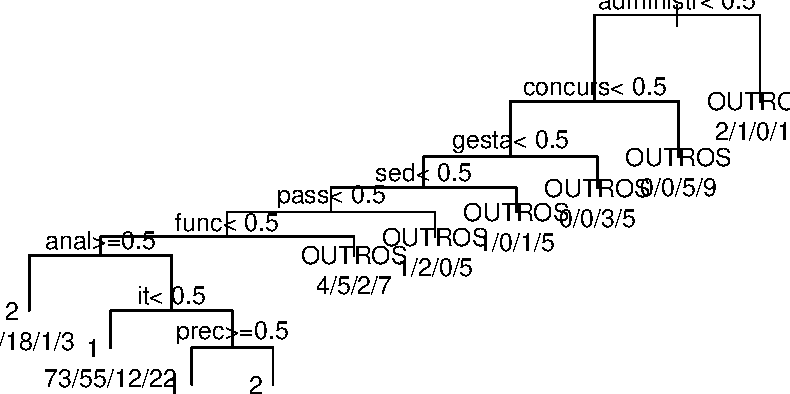
\includegraphics{markdown_v50_files/figure-latex/unnamed-chunk-85-1.pdf}

\begin{Shaded}
\begin{Highlighting}[]
\CommentTok{# Predict the testing set with the trained model }
\NormalTok{predictions <-}\StringTok{ }\KeywordTok{predict}\NormalTok{(rf, testing, }\DataTypeTok{type =} \StringTok{"class"}\NormalTok{)}

\CommentTok{# Accuracy and other metrics}
\KeywordTok{confusionMatrix}\NormalTok{(predictions, }\KeywordTok{as.factor}\NormalTok{(testing}\OperatorTok{$}\NormalTok{DIRETORIA))}
\end{Highlighting}
\end{Shaded}

\begin{verbatim}
## Confusion Matrix and Statistics
## 
##           Reference
## Prediction  1  2  5 OUTROS
##     1      44 42  8     19
##     2      22 28  6     13
##     5       0  0  0      0
##     OUTROS  8  3  5     18
## 
## Overall Statistics
##                                           
##                Accuracy : 0.4167          
##                  95% CI : (0.3502, 0.4855)
##     No Information Rate : 0.3426          
##     P-Value [Acc > NIR] : 0.01401         
##                                           
##                   Kappa : 0.1376          
##                                           
##  Mcnemar's Test P-Value : 2.78e-06        
## 
## Statistics by Class:
## 
##                      Class: 1 Class: 2 Class: 5 Class: OUTROS
## Sensitivity            0.5946   0.3836  0.00000       0.36000
## Specificity            0.5141   0.7133  1.00000       0.90361
## Pos Pred Value         0.3894   0.4058      NaN       0.52941
## Neg Pred Value         0.7087   0.6939  0.91204       0.82418
## Prevalence             0.3426   0.3380  0.08796       0.23148
## Detection Rate         0.2037   0.1296  0.00000       0.08333
## Detection Prevalence   0.5231   0.3194  0.00000       0.15741
## Balanced Accuracy      0.5543   0.5484  0.50000       0.63181
\end{verbatim}

Olhando as 6 primeiras observações real X predito

\begin{Shaded}
\begin{Highlighting}[]
\NormalTok{p1 <-}\StringTok{ }\KeywordTok{predict}\NormalTok{(rf,training)}
\KeywordTok{head}\NormalTok{(p1)}
\end{Highlighting}
\end{Shaded}

\begin{verbatim}
##           1          2          5    OUTROS
## 1 0.4506173 0.33950617 0.07407407 0.1358025
## 2 0.5238095 0.23809524 0.14285714 0.0952381
## 3 0.3250000 0.42500000 0.08333333 0.1666667
## 4 0.5238095 0.23809524 0.14285714 0.0952381
## 5 0.4506173 0.33950617 0.07407407 0.1358025
## 6 0.1052632 0.05263158 0.00000000 0.8421053
\end{verbatim}

\begin{Shaded}
\begin{Highlighting}[]
\KeywordTok{head}\NormalTok{(training}\OperatorTok{$}\NormalTok{DIRETORIA)}
\end{Highlighting}
\end{Shaded}

\begin{verbatim}
## [1] "5"      "1"      "2"      "1"      "OUTROS" "1"
\end{verbatim}

Selecionando uma árvore

\begin{Shaded}
\begin{Highlighting}[]
\NormalTok{rp <-}\StringTok{ }\NormalTok{rpart}\OperatorTok{::}\KeywordTok{rpart}\NormalTok{(}\DataTypeTok{formula =}\NormalTok{ DIRETORIA}\OperatorTok{~}\NormalTok{.,}\DataTypeTok{data=}\NormalTok{training)}
\end{Highlighting}
\end{Shaded}

\begin{Shaded}
\begin{Highlighting}[]
\NormalTok{rpart}\OperatorTok{::}\KeywordTok{plotcp}\NormalTok{(rf)}
\end{Highlighting}
\end{Shaded}

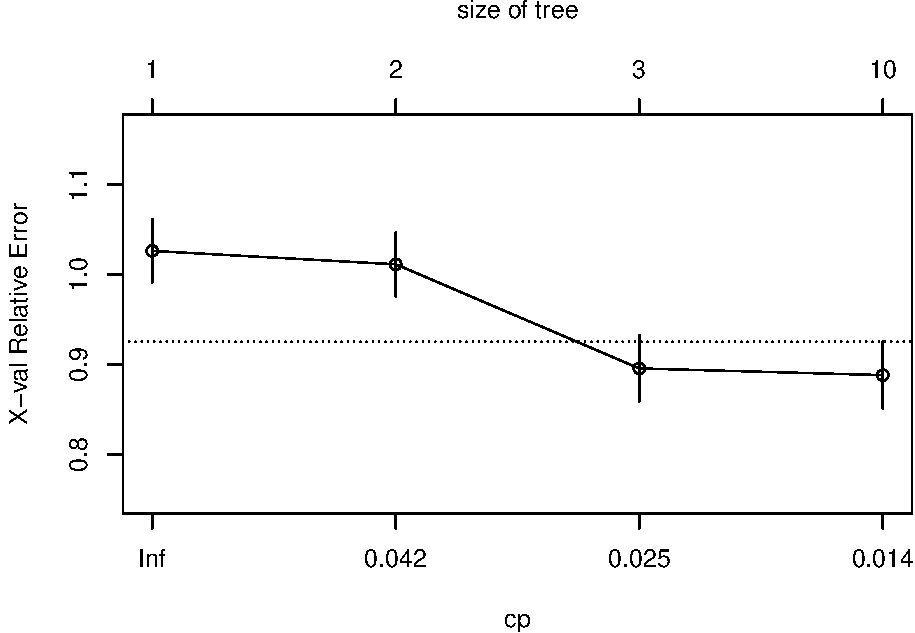
\includegraphics{markdown_v50_files/figure-latex/unnamed-chunk-89-1.pdf}

\begin{Shaded}
\begin{Highlighting}[]
\KeywordTok{rpart.plot}\NormalTok{(rf)}
\end{Highlighting}
\end{Shaded}

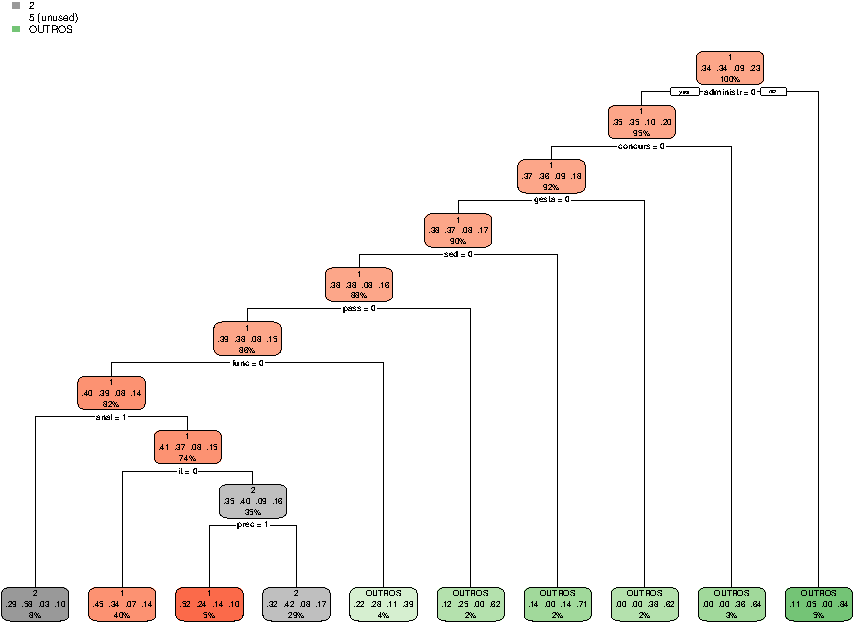
\includegraphics{markdown_v50_files/figure-latex/unnamed-chunk-89-2.pdf}

\begin{Shaded}
\begin{Highlighting}[]
\KeywordTok{rpart.plot.version1}\NormalTok{(rf)}
\end{Highlighting}
\end{Shaded}

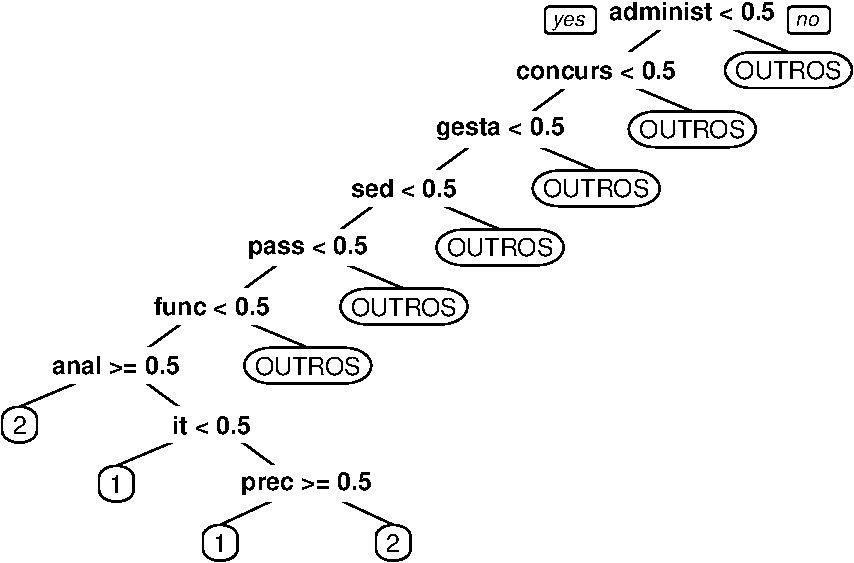
\includegraphics{markdown_v50_files/figure-latex/unnamed-chunk-89-3.pdf}

Outra forma de escrever o modelo é usando a função
\texttt{randomForest(\ )}

\begin{Shaded}
\begin{Highlighting}[]
\KeywordTok{set.seed}\NormalTok{(}\DecValTok{09986755}\NormalTok{)}
\NormalTok{rf1 <-}\StringTok{ }\KeywordTok{randomForest}\NormalTok{(}\KeywordTok{as.factor}\NormalTok{(DIRETORIA) }\OperatorTok{~}\StringTok{ }\NormalTok{., }\DataTypeTok{data=}\NormalTok{training,}
                    \DataTypeTok{importance =} \OtherTok{TRUE}\NormalTok{,}
                    \DataTypeTok{proximity =} \OtherTok{TRUE}\NormalTok{)}
\NormalTok{rf1}
\end{Highlighting}
\end{Shaded}

\begin{verbatim}
## 
## Call:
##  randomForest(formula = as.factor(DIRETORIA) ~ ., data = training,      importance = TRUE, proximity = TRUE) 
##                Type of random forest: classification
##                      Number of trees: 500
## No. of variables tried at each split: 6
## 
##         OOB estimate of  error rate: 51.96%
## Confusion matrix:
##         1  2 5 OUTROS class.error
## 1      82 50 0      8   0.4142857
## 2      64 68 0      5   0.5036496
## 5      16 11 2      8   0.9459459
## OUTROS 25 20 5     44   0.5319149
\end{verbatim}

\begin{Shaded}
\begin{Highlighting}[]
\CommentTok{# Predict the testing set with the trained model}
\NormalTok{predictions1 <-}\StringTok{ }\KeywordTok{predict}\NormalTok{(rf1, testing, }\DataTypeTok{type =} \StringTok{"class"}\NormalTok{)}

\CommentTok{# Accuracy and other metrics}
\KeywordTok{confusionMatrix}\NormalTok{(predictions1, }\KeywordTok{as.factor}\NormalTok{(testing}\OperatorTok{$}\NormalTok{DIRETORIA))}
\end{Highlighting}
\end{Shaded}

\begin{verbatim}
## Confusion Matrix and Statistics
## 
##           Reference
## Prediction  1  2  5 OUTROS
##     1      45 40  8     20
##     2      25 33  6      9
##     5       2  0  0      1
##     OUTROS  2  0  5     20
## 
## Overall Statistics
##                                          
##                Accuracy : 0.4537         
##                  95% CI : (0.386, 0.5227)
##     No Information Rate : 0.3426         
##     P-Value [Acc > NIR] : 0.0004699      
##                                          
##                   Kappa : 0.1923         
##                                          
##  Mcnemar's Test P-Value : 5.827e-07      
## 
## Statistics by Class:
## 
##                      Class: 1 Class: 2 Class: 5 Class: OUTROS
## Sensitivity            0.6081   0.4521  0.00000       0.40000
## Specificity            0.5211   0.7203  0.98477       0.95783
## Pos Pred Value         0.3982   0.4521  0.00000       0.74074
## Neg Pred Value         0.7184   0.7203  0.91080       0.84127
## Prevalence             0.3426   0.3380  0.08796       0.23148
## Detection Rate         0.2083   0.1528  0.00000       0.09259
## Detection Prevalence   0.5231   0.3380  0.01389       0.12500
## Balanced Accuracy      0.5646   0.5862  0.49239       0.67892
\end{verbatim}

Importância de variáveis

\begin{Shaded}
\begin{Highlighting}[]
\NormalTok{RF_importance =}\StringTok{ }\NormalTok{randomForest}\OperatorTok{::}\KeywordTok{importance}\NormalTok{(rf1)[}\KeywordTok{order}\NormalTok{(randomForest}\OperatorTok{::}\KeywordTok{importance}\NormalTok{(rf1)[,}\DecValTok{1}\NormalTok{], }\DataTypeTok{decreasing =} \OtherTok{TRUE}\NormalTok{), ]}
\NormalTok{randomForest}\OperatorTok{::}\KeywordTok{varImpPlot}\NormalTok{(rf1)}
\end{Highlighting}
\end{Shaded}

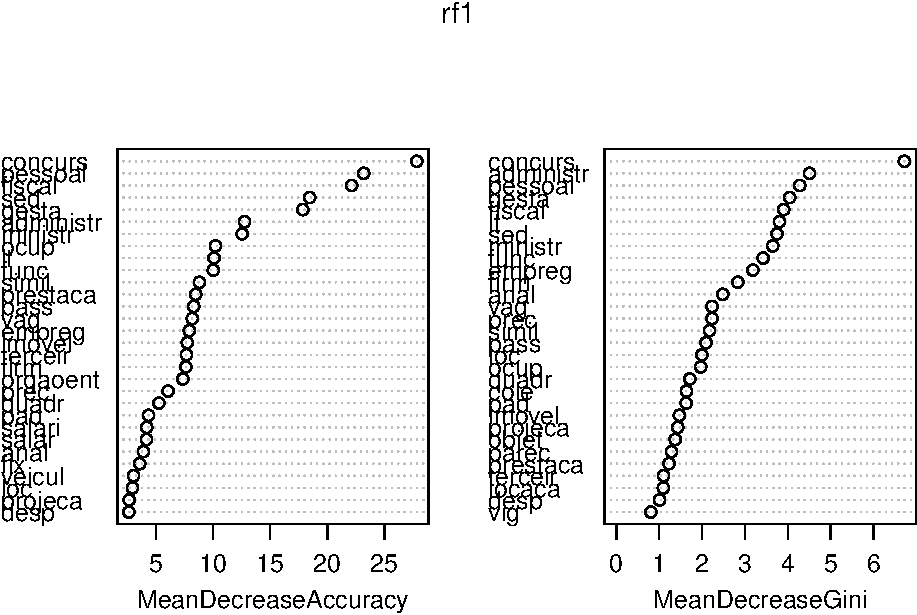
\includegraphics{markdown_v50_files/figure-latex/unnamed-chunk-91-1.pdf}

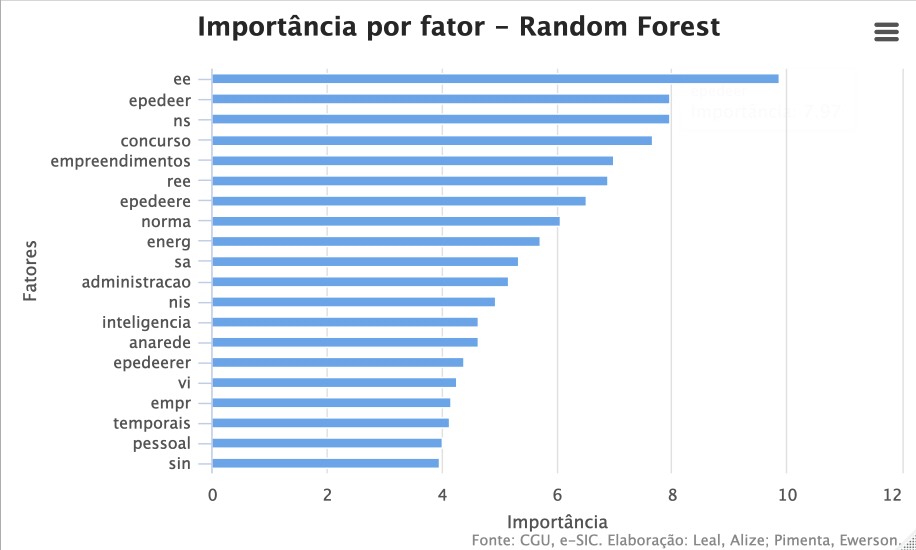
\includegraphics[width=400px]{/Users/ewersonpimenta/Desktop/ESIC_TCC/TCC_v2.1/RMARKDOWN/IMAGENS/RF_var_importance}

\begin{Shaded}
\begin{Highlighting}[]
\KeywordTok{plot}\NormalTok{(rf1)}
\KeywordTok{legend}\NormalTok{(}\StringTok{'topright'}\NormalTok{, }\KeywordTok{colnames}\NormalTok{(rf1}\OperatorTok{$}\NormalTok{err.rate), }\DataTypeTok{col=}\DecValTok{1}\OperatorTok{:}\DecValTok{5}\NormalTok{, }\DataTypeTok{fill=}\DecValTok{1}\OperatorTok{:}\DecValTok{5}\NormalTok{)}
\end{Highlighting}
\end{Shaded}

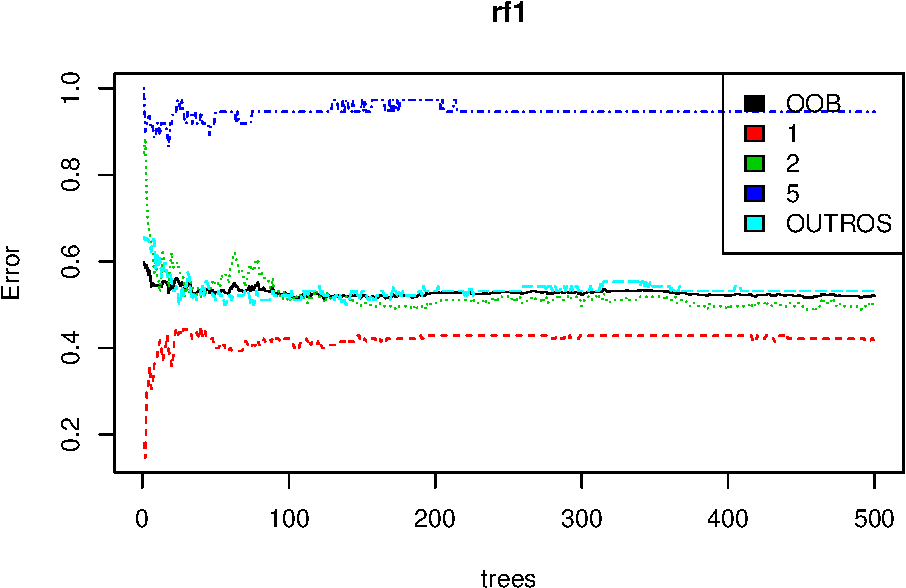
\includegraphics{markdown_v50_files/figure-latex/unnamed-chunk-93-1.pdf}

A partir de \(n=420\) árvores a taxa do erro \textbf{OOB (Out of Bag)}
tende a estabilizar.

\hypertarget{tuning-do-modelo}{%
\subparagraph{Tuning do modelo}\label{tuning-do-modelo}}

Fixando, então, \(n=420\) árvores

Aparentemente \(mtry = 26\) parece ser um bom palpite para o segundo
parâmetro do random forest, uma vez que esse retornou menor taxa de erro
\textbf{OOB}, \(27,03\%\). Entretanto esse erro ainda é muito alto.
Vamos reescrever o modelo com os parâmetros tunados.

\begin{Shaded}
\begin{Highlighting}[]
\KeywordTok{set.seed}\NormalTok{(}\DecValTok{09986755}\NormalTok{)}
\NormalTok{rf2 <-}\StringTok{ }\KeywordTok{randomForest}\NormalTok{(}\KeywordTok{as.factor}\NormalTok{(DIRETORIA) }\OperatorTok{~}\StringTok{ }\NormalTok{., }\DataTypeTok{data=}\NormalTok{training,}
                    \DataTypeTok{ntree =} \DecValTok{420}\NormalTok{,}
                    \DataTypeTok{mtry =} \DecValTok{26}\NormalTok{,}
                    \DataTypeTok{importance =} \OtherTok{TRUE}\NormalTok{,}
                    \DataTypeTok{proximity =} \OtherTok{TRUE}\NormalTok{)}
\NormalTok{rf2}
\end{Highlighting}
\end{Shaded}

\begin{verbatim}
## 
## Call:
##  randomForest(formula = as.factor(DIRETORIA) ~ ., data = training,      ntree = 420, mtry = 26, importance = TRUE, proximity = TRUE) 
##                Type of random forest: classification
##                      Number of trees: 420
## No. of variables tried at each split: 26
## 
##         OOB estimate of  error rate: 53.92%
## Confusion matrix:
##         1  2 5 OUTROS class.error
## 1      79 54 1      6   0.4357143
## 2      66 68 0      3   0.5036496
## 5      15 12 5      5   0.8648649
## OUTROS 27 23 8     36   0.6170213
\end{verbatim}

\begin{Shaded}
\begin{Highlighting}[]
\CommentTok{# Predict the testing set with the trained model}
\NormalTok{predictions2 <-}\StringTok{ }\KeywordTok{predict}\NormalTok{(rf2, testing, }\DataTypeTok{type =} \StringTok{"class"}\NormalTok{)}

\CommentTok{# Accuracy and other metrics}
\NormalTok{(}\DataTypeTok{rf2_CONFUSIONM =} \KeywordTok{confusionMatrix}\NormalTok{(predictions2, }\KeywordTok{as.factor}\NormalTok{(testing}\OperatorTok{$}\NormalTok{DIRETORIA)))}
\end{Highlighting}
\end{Shaded}

\begin{verbatim}
## Confusion Matrix and Statistics
## 
##           Reference
## Prediction  1  2  5 OUTROS
##     1      38 35  8     18
##     2      32 36  7     12
##     5       2  0  2      1
##     OUTROS  2  2  2     19
## 
## Overall Statistics
##                                           
##                Accuracy : 0.4398          
##                  95% CI : (0.3725, 0.5088)
##     No Information Rate : 0.3426          
##     P-Value [Acc > NIR] : 0.001911        
##                                           
##                   Kappa : 0.1738          
##                                           
##  Mcnemar's Test P-Value : 2.523e-05       
## 
## Statistics by Class:
## 
##                      Class: 1 Class: 2 Class: 5 Class: OUTROS
## Sensitivity            0.5135   0.4932 0.105263       0.38000
## Specificity            0.5704   0.6434 0.984772       0.96386
## Pos Pred Value         0.3838   0.4138 0.400000       0.76000
## Neg Pred Value         0.6923   0.7132 0.919431       0.83770
## Prevalence             0.3426   0.3380 0.087963       0.23148
## Detection Rate         0.1759   0.1667 0.009259       0.08796
## Detection Prevalence   0.4583   0.4028 0.023148       0.11574
## Balanced Accuracy      0.5420   0.5683 0.545017       0.67193
\end{verbatim}

\begin{Shaded}
\begin{Highlighting}[]
\NormalTok{p2 <-}\StringTok{ }\KeywordTok{predict}\NormalTok{(rf2,training)}
\KeywordTok{as.character}\NormalTok{(}\KeywordTok{head}\NormalTok{(p2))}
\end{Highlighting}
\end{Shaded}

\begin{verbatim}
## [1] "1" "1" "2" "1" "1" "1"
\end{verbatim}

\begin{Shaded}
\begin{Highlighting}[]
\KeywordTok{head}\NormalTok{(training}\OperatorTok{$}\NormalTok{DIRETORIA)}
\end{Highlighting}
\end{Shaded}

\begin{verbatim}
## [1] "5"      "1"      "2"      "1"      "OUTROS" "1"
\end{verbatim}

\begin{Shaded}
\begin{Highlighting}[]
\NormalTok{(}\DataTypeTok{DEA_erroCLASS =} \KeywordTok{sum}\NormalTok{(rf2_CONFUSIONM}\OperatorTok{$}\NormalTok{table[}\DecValTok{1}\NormalTok{,}\DecValTok{2}\OperatorTok{:}\DecValTok{3}\NormalTok{])}\OperatorTok{/}\StringTok{ }\KeywordTok{sum}\NormalTok{(rf2_CONFUSIONM}\OperatorTok{$}\NormalTok{table[}\DecValTok{1}\NormalTok{,]))}
\end{Highlighting}
\end{Shaded}

\begin{verbatim}
## [1] 0.4343434
\end{verbatim}

\begin{Shaded}
\begin{Highlighting}[]
\NormalTok{(}\DataTypeTok{DEE_erroCLASS =} \KeywordTok{sum}\NormalTok{(rf2_CONFUSIONM}\OperatorTok{$}\NormalTok{table[}\DecValTok{2}\NormalTok{,}\KeywordTok{c}\NormalTok{(}\DecValTok{1}\NormalTok{,}\DecValTok{3}\NormalTok{)])}\OperatorTok{/}\StringTok{ }\KeywordTok{sum}\NormalTok{(rf2_CONFUSIONM}\OperatorTok{$}\NormalTok{table[}\DecValTok{2}\NormalTok{,]))}
\end{Highlighting}
\end{Shaded}

\begin{verbatim}
## [1] 0.4482759
\end{verbatim}

\begin{Shaded}
\begin{Highlighting}[]
\NormalTok{(}\DataTypeTok{OUTROS_erroCLASS =} \KeywordTok{sum}\NormalTok{(rf2_CONFUSIONM}\OperatorTok{$}\NormalTok{table[}\DecValTok{3}\NormalTok{,}\DecValTok{1}\OperatorTok{:}\DecValTok{2}\NormalTok{])}\OperatorTok{/}\StringTok{ }\KeywordTok{sum}\NormalTok{(rf2_CONFUSIONM}\OperatorTok{$}\NormalTok{table[}\DecValTok{3}\NormalTok{,]))}
\end{Highlighting}
\end{Shaded}

\begin{verbatim}
## [1] 0.4
\end{verbatim}

Acurácia de aproximadamente \(72\%\) na base de teste. E as taxas de
erro de classificação foram 30\%, 44\% e 45\% para \emph{DEA},
\emph{DEE} e \emph{OUTROS}, respectivamente. Houve um melhor desempenho
na classificação do modelo para a categoria \emph{DEA}

\begin{Shaded}
\begin{Highlighting}[]
\NormalTok{RF_importance =}\StringTok{ }\NormalTok{randomForest}\OperatorTok{::}\KeywordTok{importance}\NormalTok{(rf2)[}\KeywordTok{order}\NormalTok{(randomForest}\OperatorTok{::}\KeywordTok{importance}\NormalTok{(rf2)[,}\DecValTok{1}\NormalTok{], }\DataTypeTok{decreasing =} \OtherTok{TRUE}\NormalTok{), ]}
\NormalTok{randomForest}\OperatorTok{::}\KeywordTok{varImpPlot}\NormalTok{(rf2)}
\end{Highlighting}
\end{Shaded}

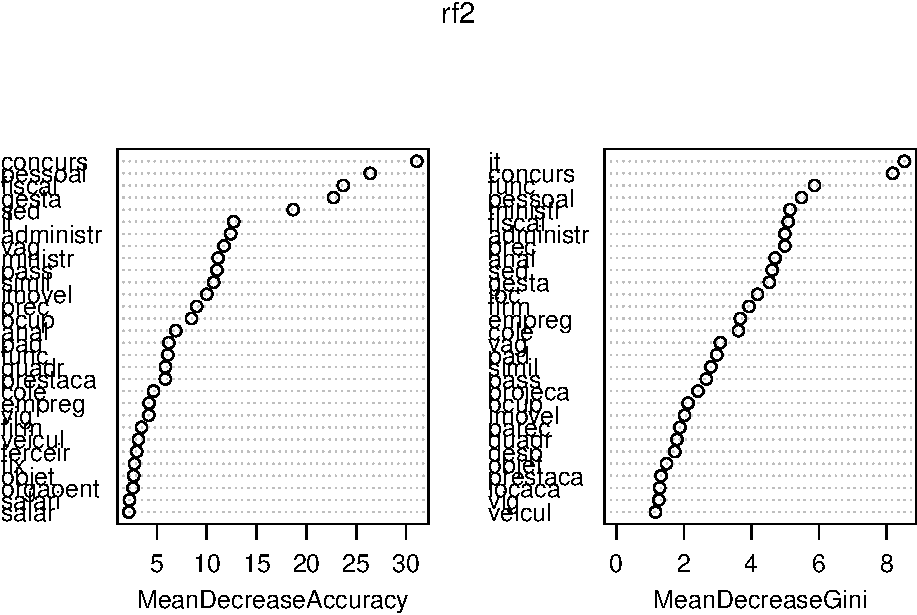
\includegraphics{markdown_v50_files/figure-latex/unnamed-chunk-97-1.pdf}

Taxa de Erro Random Forest

\begin{Shaded}
\begin{Highlighting}[]
\KeywordTok{plot}\NormalTok{(rf2, }\DataTypeTok{main =} \StringTok{"Taxa de erro OOB - Out of Bag"}\NormalTok{)}
\KeywordTok{legend}\NormalTok{(}\StringTok{'topright'}\NormalTok{, }\KeywordTok{colnames}\NormalTok{(rf2}\OperatorTok{$}\NormalTok{err.rate), }\DataTypeTok{col=}\DecValTok{1}\OperatorTok{:}\DecValTok{5}\NormalTok{, }\DataTypeTok{fill=}\DecValTok{1}\OperatorTok{:}\DecValTok{5}\NormalTok{)}
\end{Highlighting}
\end{Shaded}

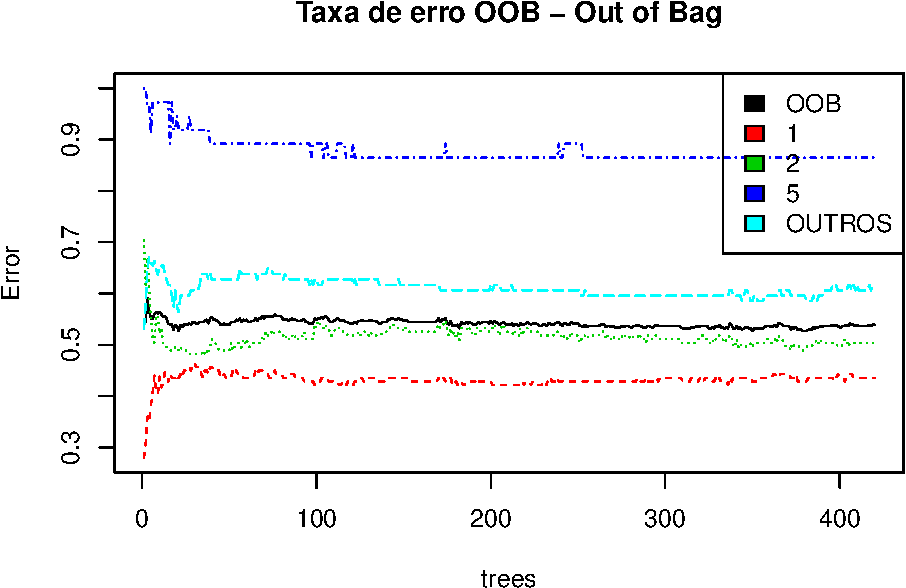
\includegraphics{markdown_v50_files/figure-latex/unnamed-chunk-98-1.pdf}

Histograma do Número de nós por árvore

\begin{Shaded}
\begin{Highlighting}[]
\KeywordTok{hist}\NormalTok{(}\KeywordTok{treesize}\NormalTok{(rf2), }\DataTypeTok{probability =}\NormalTok{ T,}
     \DataTypeTok{main =} \StringTok{"Distribuição do nº de nós por ávore"}\NormalTok{,}
     \DataTypeTok{col =} \StringTok{"pink"}\NormalTok{)}
\end{Highlighting}
\end{Shaded}

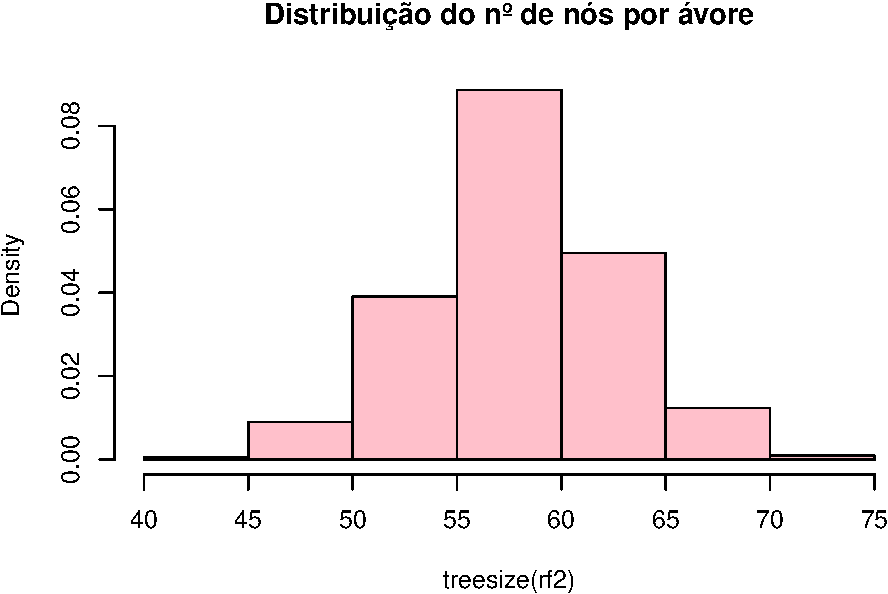
\includegraphics{markdown_v50_files/figure-latex/unnamed-chunk-99-1.pdf}

Vamos excluir as variáveis que não retornaram valor de importância para
o algoritmo do random forest.

\begin{Shaded}
\begin{Highlighting}[]
\NormalTok{RF_importance =}\StringTok{ }\NormalTok{randomForest}\OperatorTok{::}\KeywordTok{importance}\NormalTok{(rf2)[}\KeywordTok{order}\NormalTok{(randomForest}\OperatorTok{::}\KeywordTok{importance}\NormalTok{(rf2)[,}\DecValTok{1}\NormalTok{], }\DataTypeTok{decreasing =} \OtherTok{TRUE}\NormalTok{), ]}
\end{Highlighting}
\end{Shaded}

\begin{Shaded}
\begin{Highlighting}[]
\NormalTok{RF1 =}\StringTok{ }\KeywordTok{data.frame}\NormalTok{(}\DataTypeTok{variables =} \KeywordTok{rownames}\NormalTok{(RF_importance), }\DataTypeTok{importance =}\NormalTok{ RF_importance[,}\DecValTok{4}\NormalTok{])}
\NormalTok{RF1 =}\StringTok{ }\NormalTok{RF1[}\KeywordTok{order}\NormalTok{(RF1}\OperatorTok{$}\NormalTok{importance, }\DataTypeTok{decreasing =} \OtherTok{TRUE}\NormalTok{),]}
\KeywordTok{rownames}\NormalTok{(RF1) <-}\StringTok{ }\OtherTok{NULL}
\CommentTok{#summary(RF1)}
\end{Highlighting}
\end{Shaded}

\begin{Shaded}
\begin{Highlighting}[]
\FunctionTok{RF2 = RF1[1:}\AttributeTok{20,]}
\CommentTok{#library("highcharter")}
\NormalTok{hc6_1 <- highchart() %>%}
\NormalTok{  hc_add_series(data = RF2$importance, }
\NormalTok{                type = }\StringTok{"bar"}\NormalTok{,}
\NormalTok{                name = }\StringTok{"Importância"}\NormalTok{,}
\NormalTok{                showInLegend = FALSE,}
\NormalTok{                tooltip = list(valueDecimals = 2, valuePrefix = }\StringTok{""}\NormalTok{, valueSuffix = }\StringTok{""}\NormalTok{)) %>%}
\NormalTok{  hc_yAxis(title = list(text = }\StringTok{"Importância"}\NormalTok{), }
\NormalTok{           allowDecimals = TRUE, max = 12,}
\NormalTok{           labels = list(format = }\StringTok{"\{value\}"}\NormalTok{)) %>%}
\NormalTok{  hc_xAxis(title = list(text = }\StringTok{"Fatores"}\NormalTok{),}
\NormalTok{           categories = RF2$variables,}
\NormalTok{           tickmarkPlacement = }\StringTok{"on"}\NormalTok{,}
\NormalTok{           opposite = FALSE) %>%}
\NormalTok{  hc_title(text = }\StringTok{"Importância por fator - Random Forest"}\NormalTok{,}
\NormalTok{           style = list(fontWeight = }\StringTok{"bold"}\NormalTok{)) %>% }
\NormalTok{  hc_subtitle(text = paste(}\StringTok{""}\NormalTok{)) %>%}
\NormalTok{      hc_tooltip(valueDecimals = 2,}
                 \FunctionTok{pointFormat = "Importância:}\AttributeTok{ }\KeywordTok{\{}\NormalTok{point.y}\KeywordTok{\}}\StringTok{")%>%}
\StringTok{                 #pointFormat = "}\ErrorTok{Variável: \{point.x\} <br> Importância: \{point.y\}") }
\NormalTok{      hc_credits(enabled = TRUE, }
                 \FunctionTok{text = "Fonte:}\AttributeTok{ CGU, e-SIC. Elaboração: Leal, Alize; Pimenta, Ewerson.",}
\NormalTok{                 style = list(fontSize = }\StringTok{"10px"}\NormalTok{)) %>%}
\NormalTok{  hc_exporting(enabled = TRUE, filename = }\StringTok{"F6_1-importance-Pimenta"}\NormalTok{)}
\CommentTok{#hc <- hc %>% }
\CommentTok{#  hc_add_theme(hc_theme_darkunica())}
\NormalTok{hc6_1}
\end{Highlighting}
\end{Shaded}

Vamos excluir todas as variáveis que retornaram importância menor ou
igual a zero.

\begin{Shaded}
\begin{Highlighting}[]
\NormalTok{variaveis_sem_importancia =}\StringTok{ }\NormalTok{RF1 }\OperatorTok\StringTok{ }\KeywordTok{filter}\NormalTok{(}\KeywordTok{as.character}\NormalTok{(importance) }\OperatorTok{<=}\StringTok{ }\DecValTok{0}\NormalTok{)}
\CommentTok{#summary(variaveis_sem_importancia)}
\NormalTok{variaveis_sem_importancia =}\StringTok{ }\KeywordTok{as.character}\NormalTok{(variaveis_sem_importancia}\OperatorTok{$}\NormalTok{variables)}
\end{Highlighting}
\end{Shaded}

\begin{Shaded}
\begin{Highlighting}[]
\NormalTok{training1 =}\StringTok{ }\NormalTok{training }\OperatorTok\StringTok{ }\KeywordTok{select}\NormalTok{(}\OperatorTok{-}\NormalTok{(variaveis_sem_importancia))}
\NormalTok{testing1 =}\StringTok{ }\NormalTok{testing }\OperatorTok\StringTok{ }\KeywordTok{select}\NormalTok{(}\OperatorTok{-}\NormalTok{(variaveis_sem_importancia))}
\NormalTok{db_modelo1 =}\StringTok{ }\NormalTok{db_modelo }\OperatorTok\StringTok{ }\KeywordTok{select}\NormalTok{(}\OperatorTok{-}\NormalTok{(variaveis_sem_importancia))}
\end{Highlighting}
\end{Shaded}

\begin{Shaded}
\begin{Highlighting}[]
\KeywordTok{set.seed}\NormalTok{(}\DecValTok{756446}\NormalTok{) }\CommentTok{#2967}
\NormalTok{rf3 <-}\StringTok{ }\KeywordTok{randomForest}\NormalTok{(}\KeywordTok{as.factor}\NormalTok{(DIRETORIA) }\OperatorTok{~}\StringTok{ }\NormalTok{., }\DataTypeTok{data=}\NormalTok{training1,}
                    \DataTypeTok{ntree =} \DecValTok{420}\NormalTok{,}
                    \DataTypeTok{mtry =} \DecValTok{26}\NormalTok{,}
                    \DataTypeTok{importance =} \OtherTok{TRUE}\NormalTok{,}
                    \DataTypeTok{proximity =} \OtherTok{TRUE}\NormalTok{)}
\end{Highlighting}
\end{Shaded}

\begin{verbatim}
## Warning in randomForest.default(m, y, ...): invalid mtry: reset to within
## valid range
\end{verbatim}

\begin{Shaded}
\begin{Highlighting}[]
\NormalTok{rf3}
\end{Highlighting}
\end{Shaded}

\begin{verbatim}
## 
## Call:
##  randomForest(formula = as.factor(DIRETORIA) ~ ., data = training1,      ntree = 420, mtry = 26, importance = TRUE, proximity = TRUE) 
##                Type of random forest: classification
##                      Number of trees: 420
## No. of variables tried at each split: 23
## 
##         OOB estimate of  error rate: 53.43%
## Confusion matrix:
##         1  2  5 OUTROS class.error
## 1      76 57  0      7   0.4571429
## 2      63 74  0      0   0.4598540
## 5      13 14  3      7   0.9189189
## OUTROS 26 21 10     37   0.6063830
\end{verbatim}

\begin{Shaded}
\begin{Highlighting}[]
\CommentTok{# Predict the testing set with the trained model}
\NormalTok{predictions3 <-}\StringTok{ }\KeywordTok{predict}\NormalTok{(rf3, testing1[,}\OperatorTok{-}\DecValTok{1}\NormalTok{], }\DataTypeTok{type =} \StringTok{"class"}\NormalTok{)}
\CommentTok{#predict(rf3, testing1[,-1], type = "prob")}

\CommentTok{# Accuracy and other metrics}
\KeywordTok{confusionMatrix}\NormalTok{(predictions3, }\KeywordTok{as.factor}\NormalTok{(testing1}\OperatorTok{$}\NormalTok{DIRETORIA))}
\end{Highlighting}
\end{Shaded}

\begin{verbatim}
## Confusion Matrix and Statistics
## 
##           Reference
## Prediction  1  2  5 OUTROS
##     1      44 35  8     17
##     2      25 38  6     13
##     5       2  0  3      1
##     OUTROS  3  0  2     19
## 
## Overall Statistics
##                                           
##                Accuracy : 0.4815          
##                  95% CI : (0.4132, 0.5503)
##     No Information Rate : 0.3426          
##     P-Value [Acc > NIR] : 1.772e-05       
##                                           
##                   Kappa : 0.2359          
##                                           
##  Mcnemar's Test P-Value : 5.631e-06       
## 
## Statistics by Class:
## 
##                      Class: 1 Class: 2 Class: 5 Class: OUTROS
## Sensitivity            0.5946   0.5205  0.15789       0.38000
## Specificity            0.5775   0.6923  0.98477       0.96988
## Pos Pred Value         0.4231   0.4634  0.50000       0.79167
## Neg Pred Value         0.7321   0.7388  0.92381       0.83854
## Prevalence             0.3426   0.3380  0.08796       0.23148
## Detection Rate         0.2037   0.1759  0.01389       0.08796
## Detection Prevalence   0.4815   0.3796  0.02778       0.11111
## Balanced Accuracy      0.5860   0.6064  0.57133       0.67494
\end{verbatim}

\begin{Shaded}
\begin{Highlighting}[]
\NormalTok{p3 <-}\StringTok{ }\KeywordTok{predict}\NormalTok{(rf3,training1)}
\KeywordTok{as.character}\NormalTok{(}\KeywordTok{head}\NormalTok{(p3))}
\end{Highlighting}
\end{Shaded}

\begin{verbatim}
## [1] "1" "2" "2" "2" "1" "1"
\end{verbatim}

\begin{Shaded}
\begin{Highlighting}[]
\KeywordTok{head}\NormalTok{(training1}\OperatorTok{$}\NormalTok{DIRETORIA)}
\end{Highlighting}
\end{Shaded}

\begin{verbatim}
## [1] "5"      "1"      "2"      "1"      "OUTROS" "1"
\end{verbatim}

\begin{Shaded}
\begin{Highlighting}[]
\KeywordTok{set.seed}\NormalTok{(}\DecValTok{756446}\NormalTok{)}
\NormalTok{rf4 <-}\StringTok{ }\KeywordTok{randomForest}\NormalTok{(}\KeywordTok{as.factor}\NormalTok{(DIRETORIA) }\OperatorTok{~}\StringTok{ }\NormalTok{., }\DataTypeTok{data=}\NormalTok{db_modelo,}
                    \DataTypeTok{ntree =} \DecValTok{420}\NormalTok{,}
                    \DataTypeTok{mtry =} \DecValTok{45}\NormalTok{,}
                    \DataTypeTok{importance =} \OtherTok{TRUE}\NormalTok{,}
                    \DataTypeTok{proximity =} \OtherTok{TRUE}\NormalTok{)}
\end{Highlighting}
\end{Shaded}

\begin{verbatim}
## Warning in randomForest.default(m, y, ...): invalid mtry: reset to within
## valid range
\end{verbatim}

\begin{Shaded}
\begin{Highlighting}[]
\NormalTok{rf4}
\end{Highlighting}
\end{Shaded}

\begin{verbatim}
## 
## Call:
##  randomForest(formula = as.factor(DIRETORIA) ~ ., data = db_modelo,      ntree = 420, mtry = 45, importance = TRUE, proximity = TRUE) 
##                Type of random forest: classification
##                      Number of trees: 420
## No. of variables tried at each split: 36
## 
##         OOB estimate of  error rate: 53.04%
## Confusion matrix:
##          1   2 5 OUTROS class.error
## 1      129  72 4      9   0.3971963
## 2      104 101 0      5   0.5190476
## 5       26  17 7      6   0.8750000
## OUTROS  44  37 7     56   0.6111111
\end{verbatim}

\begin{Shaded}
\begin{Highlighting}[]
\CommentTok{# Predict the testing set with the trained model}
\NormalTok{predictions4 <-}\StringTok{ }\KeywordTok{predict}\NormalTok{(rf4, testing, }\DataTypeTok{type =} \StringTok{"class"}\NormalTok{)}

\CommentTok{# Accuracy and other metrics}
\KeywordTok{confusionMatrix}\NormalTok{(predictions4, }\KeywordTok{as.factor}\NormalTok{(testing}\OperatorTok{$}\NormalTok{DIRETORIA))}
\end{Highlighting}
\end{Shaded}

\begin{verbatim}
## Confusion Matrix and Statistics
## 
##           Reference
## Prediction  1  2  5 OUTROS
##     1      51 33  8     12
##     2      22 40  6      9
##     5       0  0  5      1
##     OUTROS  1  0  0     28
## 
## Overall Statistics
##                                           
##                Accuracy : 0.5741          
##                  95% CI : (0.5052, 0.6409)
##     No Information Rate : 0.3426          
##     P-Value [Acc > NIR] : 3.080e-12       
##                                           
##                   Kappa : 0.3746          
##                                           
##  Mcnemar's Test P-Value : 3.435e-06       
## 
## Statistics by Class:
## 
##                      Class: 1 Class: 2 Class: 5 Class: OUTROS
## Sensitivity            0.6892   0.5479  0.26316        0.5600
## Specificity            0.6268   0.7413  0.99492        0.9940
## Pos Pred Value         0.4904   0.5195  0.83333        0.9655
## Neg Pred Value         0.7946   0.7626  0.93333        0.8824
## Prevalence             0.3426   0.3380  0.08796        0.2315
## Detection Rate         0.2361   0.1852  0.02315        0.1296
## Detection Prevalence   0.4815   0.3565  0.02778        0.1343
## Balanced Accuracy      0.6580   0.6446  0.62904        0.7770
\end{verbatim}

\begin{Shaded}
\begin{Highlighting}[]
\NormalTok{p4 <-}\StringTok{ }\KeywordTok{predict}\NormalTok{(rf4,training)}
\KeywordTok{as.character}\NormalTok{(}\KeywordTok{head}\NormalTok{(p4))}
\end{Highlighting}
\end{Shaded}

\begin{verbatim}
## [1] "1" "1" "2" "1" "1" "1"
\end{verbatim}

\begin{Shaded}
\begin{Highlighting}[]
\KeywordTok{head}\NormalTok{(training}\OperatorTok{$}\NormalTok{DIRETORIA)}
\end{Highlighting}
\end{Shaded}

\begin{verbatim}
## [1] "5"      "1"      "2"      "1"      "OUTROS" "1"
\end{verbatim}

Comparacao do poder de predicao dos modelos treinados e propostos

\begin{Shaded}
\begin{Highlighting}[]
\KeywordTok{as.character}\NormalTok{(p1[}\DecValTok{1}\OperatorTok{:}\DecValTok{15}\NormalTok{])}
\end{Highlighting}
\end{Shaded}

\begin{verbatim}
##  [1] "0.450617283950617" "0.523809523809524" "0.325"            
##  [4] "0.523809523809524" "0.450617283950617" "0.105263157894737"
##  [7] "0.450617283950617" "0.523809523809524" "0.450617283950617"
## [10] "0.450617283950617" "0.105263157894737" "0.325"            
## [13] "0.325"             "0.325"             "0.450617283950617"
\end{verbatim}

\begin{Shaded}
\begin{Highlighting}[]
\KeywordTok{as.character}\NormalTok{(rf}\OperatorTok{$}\NormalTok{y[}\DecValTok{1}\OperatorTok{:}\DecValTok{15}\NormalTok{])}
\end{Highlighting}
\end{Shaded}

\begin{verbatim}
##  [1] "3" "1" "2" "1" "4" "1" "3" "1" "2" "1" "1" "1" "1" "4" "4"
\end{verbatim}

\begin{Shaded}
\begin{Highlighting}[]
\KeywordTok{as.character}\NormalTok{(p2[}\DecValTok{1}\OperatorTok{:}\DecValTok{15}\NormalTok{])}
\end{Highlighting}
\end{Shaded}

\begin{verbatim}
##  [1] "1"      "1"      "2"      "1"      "1"      "1"      "1"     
##  [8] "1"      "1"      "1"      "1"      "2"      "2"      "OUTROS"
## [15] "1"
\end{verbatim}

\begin{Shaded}
\begin{Highlighting}[]
\KeywordTok{as.character}\NormalTok{(p4[}\DecValTok{1}\OperatorTok{:}\DecValTok{15}\NormalTok{])}
\end{Highlighting}
\end{Shaded}

\begin{verbatim}
##  [1] "1"      "1"      "2"      "1"      "1"      "1"      "1"     
##  [8] "1"      "1"      "1"      "1"      "2"      "2"      "OUTROS"
## [15] "1"
\end{verbatim}

\begin{Shaded}
\begin{Highlighting}[]
\NormalTok{training}\OperatorTok{$}\NormalTok{DIRETORIA[}\DecValTok{1}\OperatorTok{:}\DecValTok{15}\NormalTok{]}
\end{Highlighting}
\end{Shaded}

\begin{verbatim}
##  [1] "5"      "1"      "2"      "1"      "OUTROS" "1"      "5"     
##  [8] "1"      "2"      "1"      "1"      "1"      "1"      "OUTROS"
## [15] "OUTROS"
\end{verbatim}

\begin{Shaded}
\begin{Highlighting}[]
\CommentTok{#edit(MDSplot)}
\NormalTok{fig.align=}\StringTok{"center"}
\NormalTok{training1}\OperatorTok{$}\NormalTok{DIRETORIA =}\StringTok{ }\KeywordTok{as.factor}\NormalTok{(training1}\OperatorTok{$}\NormalTok{DIRETORIA)}
\NormalTok{testing1}\OperatorTok{$}\NormalTok{DIRETORIA =}\StringTok{ }\KeywordTok{as.factor}\NormalTok{(testing1}\OperatorTok{$}\NormalTok{DIRETORIA)}
\NormalTok{db_modelo}\OperatorTok{$}\NormalTok{DIRETORIA =}\StringTok{ }\KeywordTok{as.factor}\NormalTok{(db_modelo}\OperatorTok{$}\NormalTok{DIRETORIA)}

\NormalTok{(}\DataTypeTok{MDIM_treino =} \KeywordTok{MDSplot}\NormalTok{(rf3, training1}\OperatorTok{$}\NormalTok{DIRETORIA, }\DataTypeTok{pch=}\DecValTok{20}\NormalTok{))}
\end{Highlighting}
\end{Shaded}

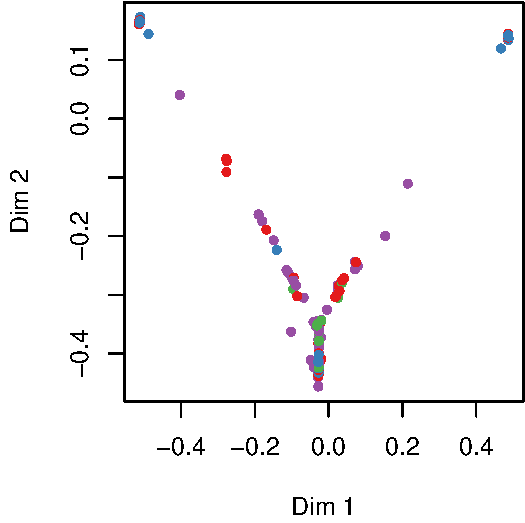
\includegraphics{markdown_v50_files/figure-latex/unnamed-chunk-107-1.pdf}

\begin{verbatim}
## $points
##           Dim 1       Dim 2
## 1    0.48706199  0.13832372
## 2   -0.51365242  0.16158370
## 3   -0.02750134 -0.42840656
## 4   -0.51421632  0.16082709
## 5    0.48679248  0.14277997
## 6   -0.02131776 -0.40854075
## 7    0.48693772  0.14015690
## 8   -0.51327875  0.16319477
## 9    0.48705865  0.14047510
## 10   0.48701012  0.13644992
## 11  -0.02117122 -0.41037581
## 12  -0.51238672  0.16591077
## 13  -0.51271311  0.16600004
## 14  -0.10991013 -0.26153938
## 15   0.01947657 -0.30229950
## 16   0.48667965  0.14432116
## 17   0.48686064  0.14103881
## 18  -0.51238717  0.16834268
## 19  -0.02699864 -0.39933997
## 20   0.04154658 -0.27156286
## 21   0.48713386  0.14038301
## 22   0.02551741 -0.30464243
## 23   0.48718274  0.13896670
## 24  -0.02648562 -0.37242162
## 25   0.48675624  0.13981756
## 26   0.48709071  0.14046916
## 27   0.48715317  0.13510545
## 28  -0.51313117  0.16543880
## 29  -0.51276292  0.16514584
## 30   0.02682511 -0.28482271
## 31  -0.02757584 -0.43194056
## 32  -0.51272403  0.16316354
## 33   0.48690474  0.14113806
## 34  -0.02865857 -0.43591082
## 35  -0.51303738  0.16424189
## 36  -0.51248334  0.16749880
## 37  -0.51215508  0.16600790
## 38  -0.10183763 -0.36258945
## 39   0.48702333  0.13658432
## 40   0.48693958  0.13649018
## 41  -0.51237553  0.16691228
## 42  -0.51234092  0.16680098
## 43  -0.02699718 -0.39929196
## 44  -0.02726683 -0.39099294
## 45  -0.02730537 -0.41886757
## 46  -0.51219454  0.16611299
## 47  -0.02850523 -0.44039193
## 48   0.48717604  0.13995521
## 49   0.02412469 -0.28381847
## 50   0.48681814  0.14171034
## 51  -0.51338052  0.16472197
## 52   0.48688923  0.13921130
## 53   0.48699855  0.14329725
## 54  -0.51225865  0.16581270
## 55   0.48712351  0.13739097
## 56   0.48690213  0.14373172
## 57  -0.51294988  0.16102077
## 58  -0.02723839 -0.39134711
## 59   0.48697233  0.14004293
## 60  -0.02695162 -0.38182752
## 61  -0.02815733 -0.34394660
## 62  -0.51216657  0.16749710
## 63  -0.02636481 -0.36192195
## 64   0.48711134  0.14052867
## 65  -0.51293719  0.16657409
## 66  -0.51261710  0.16646151
## 67  -0.51286110  0.16721306
## 68  -0.51261819  0.16534741
## 69   0.48689809  0.14003513
## 70  -0.51301522  0.16502153
## 71   0.48681471  0.13509451
## 72   0.48665569  0.14257094
## 73  -0.51285631  0.16478926
## 74   0.48689714  0.14304658
## 75  -0.51278494  0.16647662
## 76  -0.51296779  0.16372824
## 77   0.48670241  0.14252392
## 78   0.48693608  0.14052451
## 79  -0.51129826  0.16881451
## 80   0.02437334 -0.29657388
## 81   0.48686531  0.14342124
## 82  -0.02677348 -0.37428525
## 83   0.48742713  0.13940288
## 84   0.48719106  0.13718388
## 85  -0.51166458  0.16799148
## 86  -0.01981900 -0.34443188
## 87   0.48728385  0.13744844
## 88   0.48689565  0.13746035
## 89  -0.51305557  0.16272527
## 90   0.48678616  0.13935915
## 91  -0.02698745 -0.39889988
## 92  -0.27634708 -0.07189875
## 93   0.48706546  0.14057651
## 94  -0.02803162 -0.37616517
## 95  -0.51236972  0.16700094
## 96  -0.51248995  0.16771292
## 97   0.48668713  0.14096192
## 98  -0.51218448  0.16823943
## 99  -0.51247077  0.16662417
## 100  0.46752282  0.11960607
## 101 -0.51371125  0.16555960
## 102  0.48683060  0.14260857
## 103 -0.51351012  0.16167892
## 104 -0.51283980  0.16433681
## 105  0.48692979  0.14111019
## 106  0.48682207  0.14188806
## 107 -0.51198205  0.16808075
## 108 -0.51152081  0.16823935
## 109 -0.02764897 -0.41701336
## 110  0.48693682  0.14202035
## 111  0.48731521  0.13856962
## 112 -0.02677750 -0.37115267
## 113 -0.51363921  0.16334882
## 114  0.48677564  0.13951098
## 115 -0.51361237  0.16212182
## 116 -0.02658209 -0.35632541
## 117  0.01799079 -0.30383719
## 118 -0.51272649  0.16564816
## 119  0.48683120  0.13878201
## 120 -0.51267492  0.16587556
## 121 -0.02742694 -0.42470876
## 122 -0.51392212  0.16213507
## 123 -0.02879347 -0.43308084
## 124 -0.51241930  0.16410973
## 125  0.48675023  0.14353522
## 126 -0.02753120 -0.42989795
## 127  0.48706838  0.14217114
## 128  0.48712265  0.14099518
## 129  0.48710370  0.13943988
## 130  0.48685602  0.14219728
## 131  0.48733089  0.13590943
## 132 -0.14098885 -0.22321685
## 133  0.48716762  0.13835724
## 134  0.07084709 -0.25643887
## 135  0.48677467  0.13654052
## 136 -0.51252582  0.16673436
## 137  0.48688807  0.13876374
## 138 -0.51259265  0.16755862
## 139  0.48713394  0.13804966
## 140  0.48689335  0.14119695
## 141 -0.02679312 -0.38985238
## 142 -0.51175094  0.16676012
## 143 -0.02613236 -0.35592516
## 144  0.48705429  0.14231249
## 145 -0.04107436 -0.41519562
## 146 -0.02717412 -0.41263674
## 147  0.48686004  0.13979715
## 148  0.48699291  0.14004156
## 149 -0.02886886 -0.42313365
## 150  0.02501296 -0.29475983
## 151 -0.51162990  0.17031526
## 152  0.48702195  0.14039900
## 153 -0.51274420  0.16436318
## 154  0.48722826  0.13801171
## 155  0.01968680 -0.30226424
## 156 -0.02632681 -0.34668667
## 157 -0.02691977 -0.38775423
## 158 -0.02033183 -0.34543060
## 159 -0.51261479  0.16550819
## 160 -0.02865173 -0.42796055
## 161 -0.09585502 -0.29015171
## 162  0.48745620  0.13741749
## 163  0.48737790  0.13555559
## 164 -0.02863077 -0.43218836
## 165  0.48697541  0.13870282
## 166 -0.04916135 -0.41089847
## 167 -0.02639562 -0.36298240
## 168 -0.14903641 -0.20720847
## 169 -0.51305531  0.16514226
## 170 -0.02847864 -0.43882395
## 171 -0.51249729  0.16467793
## 172 -0.02879449 -0.43201723
## 173 -0.06775527 -0.30478065
## 174  0.48702931  0.14067225
## 175 -0.51275935  0.16719808
## 176 -0.51352657  0.16129565
## 177 -0.02779315 -0.38284137
## 178 -0.02807487 -0.45583784
## 179  0.07136452 -0.24386469
## 180  0.48684386  0.13918389
## 181  0.48715704  0.13719982
## 182 -0.11434129 -0.25734655
## 183 -0.10089361 -0.26946633
## 184 -0.51212758  0.16576037
## 185  0.48686902  0.14014498
## 186 -0.02744236 -0.42535800
## 187 -0.51261937  0.16571058
## 188  0.48703868  0.13783354
## 189 -0.51331720  0.16348032
## 190 -0.51312792  0.16765108
## 191 -0.01962682 -0.34283921
## 192  0.48728429  0.13859410
## 193 -0.51247188  0.16625739
## 194 -0.51304480  0.16390961
## 195 -0.02766244 -0.43581360
## 196  0.48710408  0.14173396
## 197 -0.02701554 -0.40008268
## 198 -0.18020933 -0.17451139
## 199 -0.01988743 -0.34229844
## 200  0.48670003  0.14136218
## 201  0.48683441  0.13922578
## 202 -0.51226991  0.16962762
## 203 -0.51325596  0.16629632
## 204 -0.51203049  0.16768635
## 205  0.48711727  0.14079768
## 206  0.48712167  0.13741070
## 207  0.48716227  0.13763595
## 208  0.48710292  0.13684606
## 209 -0.40387636  0.04037033
## 210 -0.51266389  0.16541010
## 211 -0.51281341  0.16555359
## 212  0.48677849  0.14145723
## 213  0.48684726  0.13547234
## 214 -0.51200852  0.16593581
## 215  0.48682317  0.13805461
## 216 -0.02755464 -0.43102921
## 217  0.48736030  0.13359581
## 218 -0.51266232  0.16714897
## 219 -0.02652428 -0.37109718
## 220 -0.04090641 -0.41806977
## 221 -0.02699519 -0.39921547
## 222  0.48729329  0.13858438
## 223 -0.51251745  0.16645630
## 224  0.48683906  0.14268678
## 225 -0.02755466 -0.43088461
## 226  0.02716698 -0.28448030
## 227 -0.51376070  0.16132913
## 228  0.48731155  0.13780587
## 229  0.48684166  0.14294897
## 230  0.48707262  0.14009725
## 231 -0.51347531  0.16423083
## 232 -0.51363359  0.16350513
## 233  0.48708318  0.13805878
## 234  0.48716188  0.13863956
## 235 -0.02770025 -0.43770354
## 236  0.48677469  0.14311460
## 237  0.03658463 -0.27908817
## 238 -0.51289085  0.16455586
## 239  0.48726335  0.13824146
## 240  0.48728391  0.13978108
## 241 -0.51240042  0.16728700
## 242 -0.51255067  0.16803133
## 243  0.48661658  0.14327695
## 244 -0.27794539 -0.06834729
## 245 -0.02670451 -0.39963091
## 246 -0.04042645 -0.42286147
## 247 -0.51308664  0.16613406
## 248 -0.51244523  0.16753746
## 249  0.48721608  0.13665123
## 250 -0.51288278  0.16522315
## 251  0.48698186  0.14368084
## 252  0.48668045  0.14265837
## 253 -0.51141931  0.16694052
## 254 -0.00453419 -0.32520622
## 255 -0.51267141  0.16733883
## 256  0.48661624  0.14016976
## 257 -0.51310350  0.16410470
## 258  0.07864277 -0.25073087
## 259  0.48691045  0.14393707
## 260  0.48734348  0.13952489
## 261 -0.51225584  0.16716570
## 262 -0.51289831  0.16586784
## 263 -0.51258181  0.16742951
## 264 -0.08511403 -0.30224045
## 265 -0.02757866 -0.43211185
## 266  0.48697287  0.13631054
## 267  0.48681327  0.14154556
## 268  0.48698168  0.14379076
## 269 -0.51305795  0.16412834
## 270  0.48707777  0.14042342
## 271 -0.02748428 -0.42754660
## 272 -0.02647677 -0.37189129
## 273  0.48687838  0.14291487
## 274  0.48696233  0.14082511
## 275 -0.51273349  0.16961432
## 276 -0.02699344 -0.39913739
## 277 -0.02730852 -0.41914205
## 278 -0.51245495  0.16489852
## 279 -0.51277281  0.16394382
## 280  0.48742279  0.13835302
## 281 -0.27716911 -0.09055552
## 282 -0.51245236  0.16676575
## 283  0.48679742  0.14373217
## 284 -0.02679408 -0.38712427
## 285 -0.51220282  0.16528078
## 286 -0.51230287  0.16663843
## 287 -0.02054016 -0.37254261
## 288  0.48684735  0.14108828
## 289 -0.51236937  0.16343541
## 290 -0.51317466  0.16501285
## 291 -0.04112937 -0.34588925
## 292 -0.02624756 -0.36120923
## 293  0.48687318  0.14058910
## 294 -0.02699516 -0.39922389
## 295  0.48684550  0.14314310
## 296  0.48694506  0.13592962
## 297 -0.02629063 -0.36303073
## 298 -0.51231005  0.16629853
## 299 -0.02662651 -0.37852043
## 300  0.48688854  0.14094432
## 301 -0.02805030 -0.41113155
## 302 -0.51264168  0.16687987
## 303 -0.51135055  0.17030416
## 304  0.48694605  0.14209908
## 305  0.48744217  0.13773746
## 306 -0.02744578 -0.42550302
## 307  0.48683741  0.14298847
## 308 -0.19025785 -0.16304372
## 309  0.48702921  0.13942301
## 310 -0.02746720 -0.42684704
## 311  0.48725663  0.13868637
## 312 -0.51243092  0.16680334
## 313  0.03659801 -0.27495730
## 314 -0.51265628  0.16573157
## 315  0.48675151  0.14032994
## 316 -0.51252227  0.16784669
## 317 -0.01965163 -0.34370677
## 318  0.48724528  0.14029093
## 319 -0.51168456  0.16922867
## 320 -0.51300243  0.16404932
## 321 -0.51206755  0.16795136
## 322  0.48724421  0.14200713
## 323 -0.03376552 -0.35394892
## 324  0.48683046  0.13894574
## 325 -0.51243970  0.16823839
## 326  0.48707520  0.13666069
## 327 -0.51247426  0.16856061
## 328  0.48675715  0.14407659
## 329 -0.51261620  0.16400547
## 330 -0.51255017  0.16624650
## 331 -0.51247536  0.16841587
## 332 -0.51301859  0.16387049
## 333 -0.02700314 -0.39956895
## 334 -0.51309135  0.16386227
## 335  0.48702901  0.13527142
## 336 -0.51204534  0.16920909
## 337  0.02937912 -0.29359522
## 338 -0.51241516  0.16826474
## 339 -0.02700374 -0.39955138
## 340 -0.51290371  0.16321342
## 341 -0.02748788 -0.42785094
## 342  0.48726679  0.13646004
## 343 -0.51282513  0.16644322
## 344  0.48712265  0.13797419
## 345 -0.48852491  0.14403628
## 346 -0.51258047  0.16689961
## 347 -0.51282179  0.16427595
## 348 -0.51220253  0.16461256
## 349  0.48708182  0.13810691
## 350  0.48678353  0.14102360
## 351 -0.02624421 -0.36100305
## 352  0.48697290  0.14221124
## 353 -0.02743446 -0.42505979
## 354  0.21438274 -0.11038038
## 355  0.48658705  0.13946612
## 356 -0.51258418  0.16887355
## 357  0.48682528  0.14276050
## 358  0.48722649  0.13412936
## 359 -0.51285970  0.16586034
## 360 -0.09505898 -0.27060771
## 361  0.48695566  0.14063531
## 362 -0.51125007  0.17314715
## 363 -0.51328656  0.16411544
## 364 -0.02660096 -0.37747199
## 365 -0.51265053  0.16379868
## 366 -0.02706361 -0.36177415
## 367  0.48661595  0.14463254
## 368 -0.02739921 -0.42327784
## 369  0.48714593  0.13669515
## 370 -0.02719841 -0.40200509
## 371  0.48675316  0.13764749
## 372  0.48693916  0.13743158
## 373  0.48715096  0.13702714
## 374 -0.16878086 -0.18892277
## 375 -0.02619131 -0.35859311
## 376 -0.51365279  0.16134746
## 377  0.48678569  0.14105265
## 378  0.48691964  0.14040297
## 379 -0.08816316 -0.28388893
## 380 -0.51294478  0.16359337
## 381  0.15290156 -0.19961962
## 382 -0.51246314  0.16724572
## 383 -0.09538355 -0.27566479
## 384  0.48688223  0.13889805
## 385 -0.51316047  0.16457519
## 386  0.48712275  0.13856442
## 387 -0.02739635 -0.42336184
## 388 -0.51121711  0.16894316
## 389  0.48725629  0.13753840
## 390 -0.02810609 -0.41421775
## 391  0.48704760  0.14004000
## 392 -0.51271540  0.16433242
## 393 -0.51278317  0.16355149
## 394 -0.51223688  0.16778839
## 395  0.48718956  0.13989236
## 396 -0.03058124 -0.34978519
## 397 -0.03125394 -0.35207884
## 398  0.48718975  0.13584490
## 399 -0.51191851  0.16934609
## 400 -0.51209990  0.16761729
## 401  0.48717265  0.13736091
## 402  0.07393553 -0.24431152
## 403 -0.51183214  0.16739802
## 404  0.48744910  0.13535988
## 405 -0.51211312  0.16581973
## 406  0.48695569  0.13833650
## 407  0.48702684  0.13967578
## 408  0.48700728  0.14215552
## 
## $eig
##   [1]  7.154072e+01  2.260444e+01  6.142944e+00  5.612111e+00  5.356335e+00
##   [6]  4.228210e+00  3.284671e+00  2.922426e+00  2.778434e+00  2.681691e+00
##  [11]  2.620385e+00  2.510296e+00  2.467015e+00  2.191005e+00  2.078947e+00
##  [16]  1.917182e+00  1.846059e+00  1.792800e+00  1.158628e+00  1.089363e+00
##  [21]  1.009891e+00  9.371735e-01  7.206314e-01  5.370035e-01  5.189383e-01
##  [26]  4.860600e-01  4.656067e-01  4.281153e-01  4.173279e-01  4.025849e-01
##  [31]  3.732467e-01  3.633766e-01  3.491361e-01  3.312614e-01  3.178951e-01
##  [36]  3.075031e-01  3.000037e-01  2.946116e-01  2.412091e-01  2.327315e-01
##  [41]  2.188737e-01  2.129291e-01  2.051127e-01  1.931579e-01  1.914391e-01
##  [46]  1.820200e-01  1.776070e-01  1.684189e-01  1.597512e-01  1.536129e-01
##  [51]  1.441120e-01  1.415717e-01  1.328320e-01  1.230696e-01  1.181261e-01
##  [56]  1.114740e-01  1.070471e-01  1.032831e-01  1.008210e-01  9.480377e-02
##  [61]  8.729672e-02  8.323205e-02  8.137579e-02  7.295963e-02  6.890010e-02
##  [66]  6.741029e-02  6.549907e-02  6.195604e-02  5.916309e-02  5.706993e-02
##  [71]  5.591420e-02  5.325271e-02  4.949706e-02  4.795811e-02  4.547968e-02
##  [76]  4.126039e-02  3.862348e-02  3.738781e-02  3.580720e-02  3.210857e-02
##  [81]  3.044963e-02  2.509894e-02  2.246196e-02  2.104936e-02  1.778965e-02
##  [86]  1.391910e-02  1.264778e-02  1.204355e-02  1.131545e-02  9.546429e-03
##  [91]  7.541357e-03  5.573194e-03  2.725189e-03  2.064650e-03  6.078363e-04
##  [96]  4.138645e-15  2.634612e-15  1.175688e-15  6.330920e-16  5.890808e-16
## [101]  5.555422e-16  5.402404e-16  5.172120e-16  4.907629e-16  4.615918e-16
## [106]  3.442972e-16  3.417240e-16  2.987823e-16  2.921588e-16  2.908981e-16
## [111]  2.622128e-16  2.611105e-16  2.364166e-16  1.913130e-16  1.790187e-16
## [116]  1.768161e-16  1.640063e-16  1.598318e-16  1.503600e-16  1.485370e-16
## [121]  1.372126e-16  1.332630e-16  1.312929e-16  1.299645e-16  1.134943e-16
## [126]  1.105201e-16  1.095396e-16  1.095218e-16  1.049813e-16  9.747550e-17
## [131]  8.969762e-17  8.102185e-17  7.953630e-17  6.845039e-17  6.039355e-17
## [136]  5.537779e-17  5.250938e-17  4.949924e-17  4.869363e-17  4.850911e-17
## [141]  4.301308e-17  3.954418e-17  3.949639e-17  3.671258e-17  3.628826e-17
## [146]  3.570248e-17  3.564546e-17  3.521152e-17  3.488612e-17  3.450431e-17
## [151]  2.988645e-17  2.671491e-17  2.645389e-17  2.613598e-17  2.484533e-17
## [156]  2.403978e-17  2.401784e-17  2.379152e-17  2.362956e-17  2.359985e-17
## [161]  2.327335e-17  2.236586e-17  2.154002e-17  2.149519e-17  2.028517e-17
## [166]  2.007724e-17  1.977315e-17  1.840639e-17  1.828335e-17  1.773784e-17
## [171]  1.631547e-17  1.628754e-17  1.614066e-17  1.602094e-17  1.596290e-17
## [176]  1.588612e-17  1.578621e-17  1.570502e-17  1.545980e-17  1.435951e-17
## [181]  1.397178e-17  1.387791e-17  1.383539e-17  1.360247e-17  1.358778e-17
## [186]  1.327493e-17  1.289235e-17  1.202899e-17  1.068537e-17  1.060518e-17
## [191]  8.424352e-18  8.386574e-18  8.060100e-18  7.920085e-18  7.090664e-18
## [196]  6.782495e-18  6.749501e-18  6.537259e-18  6.375203e-18  5.896398e-18
## [201]  5.699499e-18  5.495396e-18  5.149090e-18  4.894049e-18  4.728270e-18
## [206]  4.648356e-18  4.642101e-18  4.489704e-18  4.250791e-18  4.056572e-18
## [211]  3.416414e-18  3.160013e-18  3.102442e-18  3.002409e-18  2.857604e-18
## [216]  2.639762e-18  1.707803e-18  1.611843e-18  1.227324e-18  1.129270e-18
## [221]  9.446178e-19  8.847936e-19  7.569917e-19  6.290560e-19  5.945541e-19
## [226]  5.343330e-19  4.243650e-19 -9.359642e-19 -1.226441e-18 -2.190531e-18
## [231] -2.278966e-18 -2.340581e-18 -2.570205e-18 -2.655616e-18 -2.946622e-18
## [236] -4.910198e-18 -4.920260e-18 -4.940601e-18 -5.118634e-18 -5.390240e-18
## [241] -5.766580e-18 -5.819451e-18 -6.115810e-18 -7.519902e-18 -7.760665e-18
## [246] -8.236694e-18 -8.447660e-18 -8.452402e-18 -8.884159e-18 -8.978156e-18
## [251] -9.614729e-18 -9.624937e-18 -9.695860e-18 -1.041532e-17 -1.159739e-17
## [256] -1.186978e-17 -1.212565e-17 -1.218597e-17 -1.229858e-17 -1.274439e-17
## [261] -1.416147e-17 -1.465689e-17 -1.476018e-17 -1.541887e-17 -1.740426e-17
## [266] -1.773165e-17 -1.776412e-17 -1.835683e-17 -1.876019e-17 -1.909112e-17
## [271] -1.965292e-17 -1.988369e-17 -1.996469e-17 -2.003620e-17 -2.043187e-17
## [276] -2.044032e-17 -2.067933e-17 -2.133117e-17 -2.156873e-17 -2.186353e-17
## [281] -2.301569e-17 -2.504849e-17 -2.506474e-17 -2.565723e-17 -2.574737e-17
## [286] -2.653549e-17 -2.704155e-17 -2.956625e-17 -3.242186e-17 -3.294802e-17
## [291] -3.442858e-17 -3.507684e-17 -3.546032e-17 -3.547032e-17 -3.634026e-17
## [296] -3.859902e-17 -3.894960e-17 -4.421730e-17 -4.687827e-17 -4.808756e-17
## [301] -5.038506e-17 -5.419574e-17 -5.423806e-17 -5.994962e-17 -6.871194e-17
## [306] -8.465594e-17 -1.041368e-16 -1.185283e-16 -1.193142e-16 -1.328431e-16
## [311] -1.360447e-16 -1.860684e-16 -1.980117e-16 -2.004490e-16 -2.195498e-16
## [316] -2.204128e-16 -2.574140e-16 -3.302231e-16 -3.419604e-16 -3.422964e-16
## [321] -3.660549e-16 -5.583986e-16 -5.773028e-16 -6.745385e-16 -1.227583e-15
## [326] -1.352065e-15 -2.753607e-15 -3.571514e-15 -3.206919e-05 -8.623957e-04
## [331] -1.252205e-03 -1.545425e-03 -1.849052e-03 -2.163410e-03 -5.078032e-03
## [336] -5.698310e-03 -7.468272e-03 -8.654237e-03 -8.960363e-03 -1.093129e-02
## [341] -1.156955e-02 -1.289780e-02 -1.392421e-02 -1.759915e-02 -1.794018e-02
## [346] -2.103592e-02 -2.547492e-02 -2.662051e-02 -2.929132e-02 -3.447477e-02
## [351] -3.711743e-02 -3.803192e-02 -3.994176e-02 -4.228982e-02 -4.542149e-02
## [356] -4.775701e-02 -4.939157e-02 -5.116449e-02 -5.546252e-02 -5.848408e-02
## [361] -5.908713e-02 -6.361706e-02 -6.521525e-02 -6.789260e-02 -7.036070e-02
## [366] -7.460343e-02 -7.675212e-02 -7.811232e-02 -7.929642e-02 -8.494227e-02
## [371] -8.533985e-02 -8.748983e-02 -9.005717e-02 -9.519660e-02 -1.023627e-01
## [376] -1.055915e-01 -1.110482e-01 -1.140106e-01 -1.209387e-01 -1.239211e-01
## [381] -1.344748e-01 -1.390099e-01 -1.458075e-01 -1.608968e-01 -1.631702e-01
## [386] -1.691948e-01 -1.771840e-01 -1.832890e-01 -1.986827e-01 -2.060067e-01
## [391] -2.149887e-01 -2.215848e-01 -2.288375e-01 -2.351471e-01 -2.394344e-01
## [396] -2.547218e-01 -2.749835e-01 -2.761848e-01 -2.912567e-01 -3.011581e-01
## [401] -3.464090e-01 -3.643249e-01 -3.815793e-01 -3.987337e-01 -4.147181e-01
## [406] -4.326975e-01 -4.482354e-01 -5.330642e-01
## 
## $x
## NULL
## 
## $ac
## [1] 0
## 
## $GOF
## [1] 0.5529590 0.5875442
\end{verbatim}

\begin{Shaded}
\begin{Highlighting}[]
\NormalTok{(}\DataTypeTok{MDIM_teste =} \KeywordTok{MDSplot}\NormalTok{(rf3, testing1}\OperatorTok{$}\NormalTok{DIRETORIA, }\DataTypeTok{pch=}\DecValTok{20}\NormalTok{))}
\end{Highlighting}
\end{Shaded}

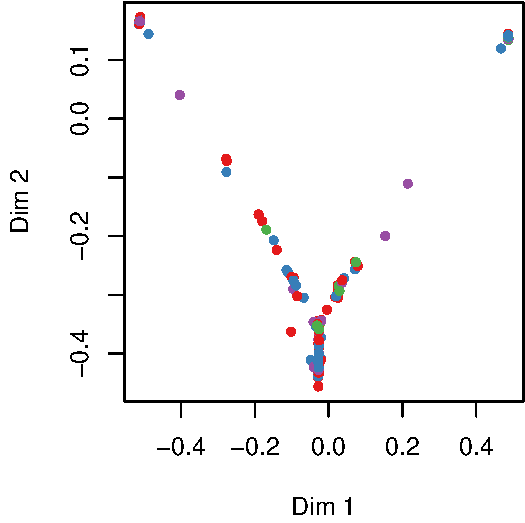
\includegraphics{markdown_v50_files/figure-latex/unnamed-chunk-107-2.pdf}

\begin{verbatim}
## $points
##           Dim 1       Dim 2
## 1    0.48706199  0.13832372
## 2   -0.51365242  0.16158370
## 3   -0.02750134 -0.42840656
## 4   -0.51421632  0.16082709
## 5    0.48679248  0.14277997
## 6   -0.02131776 -0.40854075
## 7    0.48693772  0.14015690
## 8   -0.51327875  0.16319477
## 9    0.48705865  0.14047510
## 10   0.48701012  0.13644992
## 11  -0.02117122 -0.41037581
## 12  -0.51238672  0.16591077
## 13  -0.51271311  0.16600004
## 14  -0.10991013 -0.26153938
## 15   0.01947657 -0.30229950
## 16   0.48667965  0.14432116
## 17   0.48686064  0.14103881
## 18  -0.51238717  0.16834268
## 19  -0.02699864 -0.39933997
## 20   0.04154658 -0.27156286
## 21   0.48713386  0.14038301
## 22   0.02551741 -0.30464243
## 23   0.48718274  0.13896670
## 24  -0.02648562 -0.37242162
## 25   0.48675624  0.13981756
## 26   0.48709071  0.14046916
## 27   0.48715317  0.13510545
## 28  -0.51313117  0.16543880
## 29  -0.51276292  0.16514584
## 30   0.02682511 -0.28482271
## 31  -0.02757584 -0.43194056
## 32  -0.51272403  0.16316354
## 33   0.48690474  0.14113806
## 34  -0.02865857 -0.43591082
## 35  -0.51303738  0.16424189
## 36  -0.51248334  0.16749880
## 37  -0.51215508  0.16600790
## 38  -0.10183763 -0.36258945
## 39   0.48702333  0.13658432
## 40   0.48693958  0.13649018
## 41  -0.51237553  0.16691228
## 42  -0.51234092  0.16680098
## 43  -0.02699718 -0.39929196
## 44  -0.02726683 -0.39099294
## 45  -0.02730537 -0.41886757
## 46  -0.51219454  0.16611299
## 47  -0.02850523 -0.44039193
## 48   0.48717604  0.13995521
## 49   0.02412469 -0.28381847
## 50   0.48681814  0.14171034
## 51  -0.51338052  0.16472197
## 52   0.48688923  0.13921130
## 53   0.48699855  0.14329725
## 54  -0.51225865  0.16581270
## 55   0.48712351  0.13739097
## 56   0.48690213  0.14373172
## 57  -0.51294988  0.16102077
## 58  -0.02723839 -0.39134711
## 59   0.48697233  0.14004293
## 60  -0.02695162 -0.38182752
## 61  -0.02815733 -0.34394660
## 62  -0.51216657  0.16749710
## 63  -0.02636481 -0.36192195
## 64   0.48711134  0.14052867
## 65  -0.51293719  0.16657409
## 66  -0.51261710  0.16646151
## 67  -0.51286110  0.16721306
## 68  -0.51261819  0.16534741
## 69   0.48689809  0.14003513
## 70  -0.51301522  0.16502153
## 71   0.48681471  0.13509451
## 72   0.48665569  0.14257094
## 73  -0.51285631  0.16478926
## 74   0.48689714  0.14304658
## 75  -0.51278494  0.16647662
## 76  -0.51296779  0.16372824
## 77   0.48670241  0.14252392
## 78   0.48693608  0.14052451
## 79  -0.51129826  0.16881451
## 80   0.02437334 -0.29657388
## 81   0.48686531  0.14342124
## 82  -0.02677348 -0.37428525
## 83   0.48742713  0.13940288
## 84   0.48719106  0.13718388
## 85  -0.51166458  0.16799148
## 86  -0.01981900 -0.34443188
## 87   0.48728385  0.13744844
## 88   0.48689565  0.13746035
## 89  -0.51305557  0.16272527
## 90   0.48678616  0.13935915
## 91  -0.02698745 -0.39889988
## 92  -0.27634708 -0.07189875
## 93   0.48706546  0.14057651
## 94  -0.02803162 -0.37616517
## 95  -0.51236972  0.16700094
## 96  -0.51248995  0.16771292
## 97   0.48668713  0.14096192
## 98  -0.51218448  0.16823943
## 99  -0.51247077  0.16662417
## 100  0.46752282  0.11960607
## 101 -0.51371125  0.16555960
## 102  0.48683060  0.14260857
## 103 -0.51351012  0.16167892
## 104 -0.51283980  0.16433681
## 105  0.48692979  0.14111019
## 106  0.48682207  0.14188806
## 107 -0.51198205  0.16808075
## 108 -0.51152081  0.16823935
## 109 -0.02764897 -0.41701336
## 110  0.48693682  0.14202035
## 111  0.48731521  0.13856962
## 112 -0.02677750 -0.37115267
## 113 -0.51363921  0.16334882
## 114  0.48677564  0.13951098
## 115 -0.51361237  0.16212182
## 116 -0.02658209 -0.35632541
## 117  0.01799079 -0.30383719
## 118 -0.51272649  0.16564816
## 119  0.48683120  0.13878201
## 120 -0.51267492  0.16587556
## 121 -0.02742694 -0.42470876
## 122 -0.51392212  0.16213507
## 123 -0.02879347 -0.43308084
## 124 -0.51241930  0.16410973
## 125  0.48675023  0.14353522
## 126 -0.02753120 -0.42989795
## 127  0.48706838  0.14217114
## 128  0.48712265  0.14099518
## 129  0.48710370  0.13943988
## 130  0.48685602  0.14219728
## 131  0.48733089  0.13590943
## 132 -0.14098885 -0.22321685
## 133  0.48716762  0.13835724
## 134  0.07084709 -0.25643887
## 135  0.48677467  0.13654052
## 136 -0.51252582  0.16673436
## 137  0.48688807  0.13876374
## 138 -0.51259265  0.16755862
## 139  0.48713394  0.13804966
## 140  0.48689335  0.14119695
## 141 -0.02679312 -0.38985238
## 142 -0.51175094  0.16676012
## 143 -0.02613236 -0.35592516
## 144  0.48705429  0.14231249
## 145 -0.04107436 -0.41519562
## 146 -0.02717412 -0.41263674
## 147  0.48686004  0.13979715
## 148  0.48699291  0.14004156
## 149 -0.02886886 -0.42313365
## 150  0.02501296 -0.29475983
## 151 -0.51162990  0.17031526
## 152  0.48702195  0.14039900
## 153 -0.51274420  0.16436318
## 154  0.48722826  0.13801171
## 155  0.01968680 -0.30226424
## 156 -0.02632681 -0.34668667
## 157 -0.02691977 -0.38775423
## 158 -0.02033183 -0.34543060
## 159 -0.51261479  0.16550819
## 160 -0.02865173 -0.42796055
## 161 -0.09585502 -0.29015171
## 162  0.48745620  0.13741749
## 163  0.48737790  0.13555559
## 164 -0.02863077 -0.43218836
## 165  0.48697541  0.13870282
## 166 -0.04916135 -0.41089847
## 167 -0.02639562 -0.36298240
## 168 -0.14903641 -0.20720847
## 169 -0.51305531  0.16514226
## 170 -0.02847864 -0.43882395
## 171 -0.51249729  0.16467793
## 172 -0.02879449 -0.43201723
## 173 -0.06775527 -0.30478065
## 174  0.48702931  0.14067225
## 175 -0.51275935  0.16719808
## 176 -0.51352657  0.16129565
## 177 -0.02779315 -0.38284137
## 178 -0.02807487 -0.45583784
## 179  0.07136452 -0.24386469
## 180  0.48684386  0.13918389
## 181  0.48715704  0.13719982
## 182 -0.11434129 -0.25734655
## 183 -0.10089361 -0.26946633
## 184 -0.51212758  0.16576037
## 185  0.48686902  0.14014498
## 186 -0.02744236 -0.42535800
## 187 -0.51261937  0.16571058
## 188  0.48703868  0.13783354
## 189 -0.51331720  0.16348032
## 190 -0.51312792  0.16765108
## 191 -0.01962682 -0.34283921
## 192  0.48728429  0.13859410
## 193 -0.51247188  0.16625739
## 194 -0.51304480  0.16390961
## 195 -0.02766244 -0.43581360
## 196  0.48710408  0.14173396
## 197 -0.02701554 -0.40008268
## 198 -0.18020933 -0.17451139
## 199 -0.01988743 -0.34229844
## 200  0.48670003  0.14136218
## 201  0.48683441  0.13922578
## 202 -0.51226991  0.16962762
## 203 -0.51325596  0.16629632
## 204 -0.51203049  0.16768635
## 205  0.48711727  0.14079768
## 206  0.48712167  0.13741070
## 207  0.48716227  0.13763595
## 208  0.48710292  0.13684606
## 209 -0.40387636  0.04037033
## 210 -0.51266389  0.16541010
## 211 -0.51281341  0.16555359
## 212  0.48677849  0.14145723
## 213  0.48684726  0.13547234
## 214 -0.51200852  0.16593581
## 215  0.48682317  0.13805461
## 216 -0.02755464 -0.43102921
## 217  0.48736030  0.13359581
## 218 -0.51266232  0.16714897
## 219 -0.02652428 -0.37109718
## 220 -0.04090641 -0.41806977
## 221 -0.02699519 -0.39921547
## 222  0.48729329  0.13858438
## 223 -0.51251745  0.16645630
## 224  0.48683906  0.14268678
## 225 -0.02755466 -0.43088461
## 226  0.02716698 -0.28448030
## 227 -0.51376070  0.16132913
## 228  0.48731155  0.13780587
## 229  0.48684166  0.14294897
## 230  0.48707262  0.14009725
## 231 -0.51347531  0.16423083
## 232 -0.51363359  0.16350513
## 233  0.48708318  0.13805878
## 234  0.48716188  0.13863956
## 235 -0.02770025 -0.43770354
## 236  0.48677469  0.14311460
## 237  0.03658463 -0.27908817
## 238 -0.51289085  0.16455586
## 239  0.48726335  0.13824146
## 240  0.48728391  0.13978108
## 241 -0.51240042  0.16728700
## 242 -0.51255067  0.16803133
## 243  0.48661658  0.14327695
## 244 -0.27794539 -0.06834729
## 245 -0.02670451 -0.39963091
## 246 -0.04042645 -0.42286147
## 247 -0.51308664  0.16613406
## 248 -0.51244523  0.16753746
## 249  0.48721608  0.13665123
## 250 -0.51288278  0.16522315
## 251  0.48698186  0.14368084
## 252  0.48668045  0.14265837
## 253 -0.51141931  0.16694052
## 254 -0.00453419 -0.32520622
## 255 -0.51267141  0.16733883
## 256  0.48661624  0.14016976
## 257 -0.51310350  0.16410470
## 258  0.07864277 -0.25073087
## 259  0.48691045  0.14393707
## 260  0.48734348  0.13952489
## 261 -0.51225584  0.16716570
## 262 -0.51289831  0.16586784
## 263 -0.51258181  0.16742951
## 264 -0.08511403 -0.30224045
## 265 -0.02757866 -0.43211185
## 266  0.48697287  0.13631054
## 267  0.48681327  0.14154556
## 268  0.48698168  0.14379076
## 269 -0.51305795  0.16412834
## 270  0.48707777  0.14042342
## 271 -0.02748428 -0.42754660
## 272 -0.02647677 -0.37189129
## 273  0.48687838  0.14291487
## 274  0.48696233  0.14082511
## 275 -0.51273349  0.16961432
## 276 -0.02699344 -0.39913739
## 277 -0.02730852 -0.41914205
## 278 -0.51245495  0.16489852
## 279 -0.51277281  0.16394382
## 280  0.48742279  0.13835302
## 281 -0.27716911 -0.09055552
## 282 -0.51245236  0.16676575
## 283  0.48679742  0.14373217
## 284 -0.02679408 -0.38712427
## 285 -0.51220282  0.16528078
## 286 -0.51230287  0.16663843
## 287 -0.02054016 -0.37254261
## 288  0.48684735  0.14108828
## 289 -0.51236937  0.16343541
## 290 -0.51317466  0.16501285
## 291 -0.04112937 -0.34588925
## 292 -0.02624756 -0.36120923
## 293  0.48687318  0.14058910
## 294 -0.02699516 -0.39922389
## 295  0.48684550  0.14314310
## 296  0.48694506  0.13592962
## 297 -0.02629063 -0.36303073
## 298 -0.51231005  0.16629853
## 299 -0.02662651 -0.37852043
## 300  0.48688854  0.14094432
## 301 -0.02805030 -0.41113155
## 302 -0.51264168  0.16687987
## 303 -0.51135055  0.17030416
## 304  0.48694605  0.14209908
## 305  0.48744217  0.13773746
## 306 -0.02744578 -0.42550302
## 307  0.48683741  0.14298847
## 308 -0.19025785 -0.16304372
## 309  0.48702921  0.13942301
## 310 -0.02746720 -0.42684704
## 311  0.48725663  0.13868637
## 312 -0.51243092  0.16680334
## 313  0.03659801 -0.27495730
## 314 -0.51265628  0.16573157
## 315  0.48675151  0.14032994
## 316 -0.51252227  0.16784669
## 317 -0.01965163 -0.34370677
## 318  0.48724528  0.14029093
## 319 -0.51168456  0.16922867
## 320 -0.51300243  0.16404932
## 321 -0.51206755  0.16795136
## 322  0.48724421  0.14200713
## 323 -0.03376552 -0.35394892
## 324  0.48683046  0.13894574
## 325 -0.51243970  0.16823839
## 326  0.48707520  0.13666069
## 327 -0.51247426  0.16856061
## 328  0.48675715  0.14407659
## 329 -0.51261620  0.16400547
## 330 -0.51255017  0.16624650
## 331 -0.51247536  0.16841587
## 332 -0.51301859  0.16387049
## 333 -0.02700314 -0.39956895
## 334 -0.51309135  0.16386227
## 335  0.48702901  0.13527142
## 336 -0.51204534  0.16920909
## 337  0.02937912 -0.29359522
## 338 -0.51241516  0.16826474
## 339 -0.02700374 -0.39955138
## 340 -0.51290371  0.16321342
## 341 -0.02748788 -0.42785094
## 342  0.48726679  0.13646004
## 343 -0.51282513  0.16644322
## 344  0.48712265  0.13797419
## 345 -0.48852491  0.14403628
## 346 -0.51258047  0.16689961
## 347 -0.51282179  0.16427595
## 348 -0.51220253  0.16461256
## 349  0.48708182  0.13810691
## 350  0.48678353  0.14102360
## 351 -0.02624421 -0.36100305
## 352  0.48697290  0.14221124
## 353 -0.02743446 -0.42505979
## 354  0.21438274 -0.11038038
## 355  0.48658705  0.13946612
## 356 -0.51258418  0.16887355
## 357  0.48682528  0.14276050
## 358  0.48722649  0.13412936
## 359 -0.51285970  0.16586034
## 360 -0.09505898 -0.27060771
## 361  0.48695566  0.14063531
## 362 -0.51125007  0.17314715
## 363 -0.51328656  0.16411544
## 364 -0.02660096 -0.37747199
## 365 -0.51265053  0.16379868
## 366 -0.02706361 -0.36177415
## 367  0.48661595  0.14463254
## 368 -0.02739921 -0.42327784
## 369  0.48714593  0.13669515
## 370 -0.02719841 -0.40200509
## 371  0.48675316  0.13764749
## 372  0.48693916  0.13743158
## 373  0.48715096  0.13702714
## 374 -0.16878086 -0.18892277
## 375 -0.02619131 -0.35859311
## 376 -0.51365279  0.16134746
## 377  0.48678569  0.14105265
## 378  0.48691964  0.14040297
## 379 -0.08816316 -0.28388893
## 380 -0.51294478  0.16359337
## 381  0.15290156 -0.19961962
## 382 -0.51246314  0.16724572
## 383 -0.09538355 -0.27566479
## 384  0.48688223  0.13889805
## 385 -0.51316047  0.16457519
## 386  0.48712275  0.13856442
## 387 -0.02739635 -0.42336184
## 388 -0.51121711  0.16894316
## 389  0.48725629  0.13753840
## 390 -0.02810609 -0.41421775
## 391  0.48704760  0.14004000
## 392 -0.51271540  0.16433242
## 393 -0.51278317  0.16355149
## 394 -0.51223688  0.16778839
## 395  0.48718956  0.13989236
## 396 -0.03058124 -0.34978519
## 397 -0.03125394 -0.35207884
## 398  0.48718975  0.13584490
## 399 -0.51191851  0.16934609
## 400 -0.51209990  0.16761729
## 401  0.48717265  0.13736091
## 402  0.07393553 -0.24431152
## 403 -0.51183214  0.16739802
## 404  0.48744910  0.13535988
## 405 -0.51211312  0.16581973
## 406  0.48695569  0.13833650
## 407  0.48702684  0.13967578
## 408  0.48700728  0.14215552
## 
## $eig
##   [1]  7.154072e+01  2.260444e+01  6.142944e+00  5.612111e+00  5.356335e+00
##   [6]  4.228210e+00  3.284671e+00  2.922426e+00  2.778434e+00  2.681691e+00
##  [11]  2.620385e+00  2.510296e+00  2.467015e+00  2.191005e+00  2.078947e+00
##  [16]  1.917182e+00  1.846059e+00  1.792800e+00  1.158628e+00  1.089363e+00
##  [21]  1.009891e+00  9.371735e-01  7.206314e-01  5.370035e-01  5.189383e-01
##  [26]  4.860600e-01  4.656067e-01  4.281153e-01  4.173279e-01  4.025849e-01
##  [31]  3.732467e-01  3.633766e-01  3.491361e-01  3.312614e-01  3.178951e-01
##  [36]  3.075031e-01  3.000037e-01  2.946116e-01  2.412091e-01  2.327315e-01
##  [41]  2.188737e-01  2.129291e-01  2.051127e-01  1.931579e-01  1.914391e-01
##  [46]  1.820200e-01  1.776070e-01  1.684189e-01  1.597512e-01  1.536129e-01
##  [51]  1.441120e-01  1.415717e-01  1.328320e-01  1.230696e-01  1.181261e-01
##  [56]  1.114740e-01  1.070471e-01  1.032831e-01  1.008210e-01  9.480377e-02
##  [61]  8.729672e-02  8.323205e-02  8.137579e-02  7.295963e-02  6.890010e-02
##  [66]  6.741029e-02  6.549907e-02  6.195604e-02  5.916309e-02  5.706993e-02
##  [71]  5.591420e-02  5.325271e-02  4.949706e-02  4.795811e-02  4.547968e-02
##  [76]  4.126039e-02  3.862348e-02  3.738781e-02  3.580720e-02  3.210857e-02
##  [81]  3.044963e-02  2.509894e-02  2.246196e-02  2.104936e-02  1.778965e-02
##  [86]  1.391910e-02  1.264778e-02  1.204355e-02  1.131545e-02  9.546429e-03
##  [91]  7.541357e-03  5.573194e-03  2.725189e-03  2.064650e-03  6.078363e-04
##  [96]  4.138645e-15  2.634612e-15  1.175688e-15  6.330920e-16  5.890808e-16
## [101]  5.555422e-16  5.402404e-16  5.172120e-16  4.907629e-16  4.615918e-16
## [106]  3.442972e-16  3.417240e-16  2.987823e-16  2.921588e-16  2.908981e-16
## [111]  2.622128e-16  2.611105e-16  2.364166e-16  1.913130e-16  1.790187e-16
## [116]  1.768161e-16  1.640063e-16  1.598318e-16  1.503600e-16  1.485370e-16
## [121]  1.372126e-16  1.332630e-16  1.312929e-16  1.299645e-16  1.134943e-16
## [126]  1.105201e-16  1.095396e-16  1.095218e-16  1.049813e-16  9.747550e-17
## [131]  8.969762e-17  8.102185e-17  7.953630e-17  6.845039e-17  6.039355e-17
## [136]  5.537779e-17  5.250938e-17  4.949924e-17  4.869363e-17  4.850911e-17
## [141]  4.301308e-17  3.954418e-17  3.949639e-17  3.671258e-17  3.628826e-17
## [146]  3.570248e-17  3.564546e-17  3.521152e-17  3.488612e-17  3.450431e-17
## [151]  2.988645e-17  2.671491e-17  2.645389e-17  2.613598e-17  2.484533e-17
## [156]  2.403978e-17  2.401784e-17  2.379152e-17  2.362956e-17  2.359985e-17
## [161]  2.327335e-17  2.236586e-17  2.154002e-17  2.149519e-17  2.028517e-17
## [166]  2.007724e-17  1.977315e-17  1.840639e-17  1.828335e-17  1.773784e-17
## [171]  1.631547e-17  1.628754e-17  1.614066e-17  1.602094e-17  1.596290e-17
## [176]  1.588612e-17  1.578621e-17  1.570502e-17  1.545980e-17  1.435951e-17
## [181]  1.397178e-17  1.387791e-17  1.383539e-17  1.360247e-17  1.358778e-17
## [186]  1.327493e-17  1.289235e-17  1.202899e-17  1.068537e-17  1.060518e-17
## [191]  8.424352e-18  8.386574e-18  8.060100e-18  7.920085e-18  7.090664e-18
## [196]  6.782495e-18  6.749501e-18  6.537259e-18  6.375203e-18  5.896398e-18
## [201]  5.699499e-18  5.495396e-18  5.149090e-18  4.894049e-18  4.728270e-18
## [206]  4.648356e-18  4.642101e-18  4.489704e-18  4.250791e-18  4.056572e-18
## [211]  3.416414e-18  3.160013e-18  3.102442e-18  3.002409e-18  2.857604e-18
## [216]  2.639762e-18  1.707803e-18  1.611843e-18  1.227324e-18  1.129270e-18
## [221]  9.446178e-19  8.847936e-19  7.569917e-19  6.290560e-19  5.945541e-19
## [226]  5.343330e-19  4.243650e-19 -9.359642e-19 -1.226441e-18 -2.190531e-18
## [231] -2.278966e-18 -2.340581e-18 -2.570205e-18 -2.655616e-18 -2.946622e-18
## [236] -4.910198e-18 -4.920260e-18 -4.940601e-18 -5.118634e-18 -5.390240e-18
## [241] -5.766580e-18 -5.819451e-18 -6.115810e-18 -7.519902e-18 -7.760665e-18
## [246] -8.236694e-18 -8.447660e-18 -8.452402e-18 -8.884159e-18 -8.978156e-18
## [251] -9.614729e-18 -9.624937e-18 -9.695860e-18 -1.041532e-17 -1.159739e-17
## [256] -1.186978e-17 -1.212565e-17 -1.218597e-17 -1.229858e-17 -1.274439e-17
## [261] -1.416147e-17 -1.465689e-17 -1.476018e-17 -1.541887e-17 -1.740426e-17
## [266] -1.773165e-17 -1.776412e-17 -1.835683e-17 -1.876019e-17 -1.909112e-17
## [271] -1.965292e-17 -1.988369e-17 -1.996469e-17 -2.003620e-17 -2.043187e-17
## [276] -2.044032e-17 -2.067933e-17 -2.133117e-17 -2.156873e-17 -2.186353e-17
## [281] -2.301569e-17 -2.504849e-17 -2.506474e-17 -2.565723e-17 -2.574737e-17
## [286] -2.653549e-17 -2.704155e-17 -2.956625e-17 -3.242186e-17 -3.294802e-17
## [291] -3.442858e-17 -3.507684e-17 -3.546032e-17 -3.547032e-17 -3.634026e-17
## [296] -3.859902e-17 -3.894960e-17 -4.421730e-17 -4.687827e-17 -4.808756e-17
## [301] -5.038506e-17 -5.419574e-17 -5.423806e-17 -5.994962e-17 -6.871194e-17
## [306] -8.465594e-17 -1.041368e-16 -1.185283e-16 -1.193142e-16 -1.328431e-16
## [311] -1.360447e-16 -1.860684e-16 -1.980117e-16 -2.004490e-16 -2.195498e-16
## [316] -2.204128e-16 -2.574140e-16 -3.302231e-16 -3.419604e-16 -3.422964e-16
## [321] -3.660549e-16 -5.583986e-16 -5.773028e-16 -6.745385e-16 -1.227583e-15
## [326] -1.352065e-15 -2.753607e-15 -3.571514e-15 -3.206919e-05 -8.623957e-04
## [331] -1.252205e-03 -1.545425e-03 -1.849052e-03 -2.163410e-03 -5.078032e-03
## [336] -5.698310e-03 -7.468272e-03 -8.654237e-03 -8.960363e-03 -1.093129e-02
## [341] -1.156955e-02 -1.289780e-02 -1.392421e-02 -1.759915e-02 -1.794018e-02
## [346] -2.103592e-02 -2.547492e-02 -2.662051e-02 -2.929132e-02 -3.447477e-02
## [351] -3.711743e-02 -3.803192e-02 -3.994176e-02 -4.228982e-02 -4.542149e-02
## [356] -4.775701e-02 -4.939157e-02 -5.116449e-02 -5.546252e-02 -5.848408e-02
## [361] -5.908713e-02 -6.361706e-02 -6.521525e-02 -6.789260e-02 -7.036070e-02
## [366] -7.460343e-02 -7.675212e-02 -7.811232e-02 -7.929642e-02 -8.494227e-02
## [371] -8.533985e-02 -8.748983e-02 -9.005717e-02 -9.519660e-02 -1.023627e-01
## [376] -1.055915e-01 -1.110482e-01 -1.140106e-01 -1.209387e-01 -1.239211e-01
## [381] -1.344748e-01 -1.390099e-01 -1.458075e-01 -1.608968e-01 -1.631702e-01
## [386] -1.691948e-01 -1.771840e-01 -1.832890e-01 -1.986827e-01 -2.060067e-01
## [391] -2.149887e-01 -2.215848e-01 -2.288375e-01 -2.351471e-01 -2.394344e-01
## [396] -2.547218e-01 -2.749835e-01 -2.761848e-01 -2.912567e-01 -3.011581e-01
## [401] -3.464090e-01 -3.643249e-01 -3.815793e-01 -3.987337e-01 -4.147181e-01
## [406] -4.326975e-01 -4.482354e-01 -5.330642e-01
## 
## $x
## NULL
## 
## $ac
## [1] 0
## 
## $GOF
## [1] 0.5529590 0.5875442
\end{verbatim}

\begin{Shaded}
\begin{Highlighting}[]
\NormalTok{(}\DataTypeTok{MDIM_teste =} \KeywordTok{MDSplot}\NormalTok{(rf3, db_modelo}\OperatorTok{$}\NormalTok{DIRETORIA, }\DataTypeTok{pch=}\DecValTok{20}\NormalTok{))}
\end{Highlighting}
\end{Shaded}

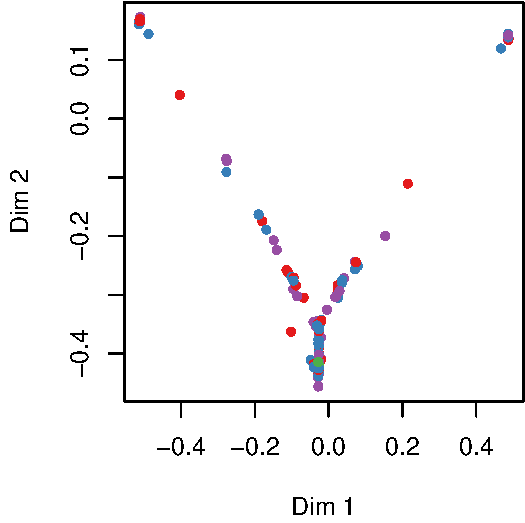
\includegraphics{markdown_v50_files/figure-latex/unnamed-chunk-107-3.pdf}

\begin{verbatim}
## $points
##           Dim 1       Dim 2
## 1    0.48706199  0.13832372
## 2   -0.51365242  0.16158370
## 3   -0.02750134 -0.42840656
## 4   -0.51421632  0.16082709
## 5    0.48679248  0.14277997
## 6   -0.02131776 -0.40854075
## 7    0.48693772  0.14015690
## 8   -0.51327875  0.16319477
## 9    0.48705865  0.14047510
## 10   0.48701012  0.13644992
## 11  -0.02117122 -0.41037581
## 12  -0.51238672  0.16591077
## 13  -0.51271311  0.16600004
## 14  -0.10991013 -0.26153938
## 15   0.01947657 -0.30229950
## 16   0.48667965  0.14432116
## 17   0.48686064  0.14103881
## 18  -0.51238717  0.16834268
## 19  -0.02699864 -0.39933997
## 20   0.04154658 -0.27156286
## 21   0.48713386  0.14038301
## 22   0.02551741 -0.30464243
## 23   0.48718274  0.13896670
## 24  -0.02648562 -0.37242162
## 25   0.48675624  0.13981756
## 26   0.48709071  0.14046916
## 27   0.48715317  0.13510545
## 28  -0.51313117  0.16543880
## 29  -0.51276292  0.16514584
## 30   0.02682511 -0.28482271
## 31  -0.02757584 -0.43194056
## 32  -0.51272403  0.16316354
## 33   0.48690474  0.14113806
## 34  -0.02865857 -0.43591082
## 35  -0.51303738  0.16424189
## 36  -0.51248334  0.16749880
## 37  -0.51215508  0.16600790
## 38  -0.10183763 -0.36258945
## 39   0.48702333  0.13658432
## 40   0.48693958  0.13649018
## 41  -0.51237553  0.16691228
## 42  -0.51234092  0.16680098
## 43  -0.02699718 -0.39929196
## 44  -0.02726683 -0.39099294
## 45  -0.02730537 -0.41886757
## 46  -0.51219454  0.16611299
## 47  -0.02850523 -0.44039193
## 48   0.48717604  0.13995521
## 49   0.02412469 -0.28381847
## 50   0.48681814  0.14171034
## 51  -0.51338052  0.16472197
## 52   0.48688923  0.13921130
## 53   0.48699855  0.14329725
## 54  -0.51225865  0.16581270
## 55   0.48712351  0.13739097
## 56   0.48690213  0.14373172
## 57  -0.51294988  0.16102077
## 58  -0.02723839 -0.39134711
## 59   0.48697233  0.14004293
## 60  -0.02695162 -0.38182752
## 61  -0.02815733 -0.34394660
## 62  -0.51216657  0.16749710
## 63  -0.02636481 -0.36192195
## 64   0.48711134  0.14052867
## 65  -0.51293719  0.16657409
## 66  -0.51261710  0.16646151
## 67  -0.51286110  0.16721306
## 68  -0.51261819  0.16534741
## 69   0.48689809  0.14003513
## 70  -0.51301522  0.16502153
## 71   0.48681471  0.13509451
## 72   0.48665569  0.14257094
## 73  -0.51285631  0.16478926
## 74   0.48689714  0.14304658
## 75  -0.51278494  0.16647662
## 76  -0.51296779  0.16372824
## 77   0.48670241  0.14252392
## 78   0.48693608  0.14052451
## 79  -0.51129826  0.16881451
## 80   0.02437334 -0.29657388
## 81   0.48686531  0.14342124
## 82  -0.02677348 -0.37428525
## 83   0.48742713  0.13940288
## 84   0.48719106  0.13718388
## 85  -0.51166458  0.16799148
## 86  -0.01981900 -0.34443188
## 87   0.48728385  0.13744844
## 88   0.48689565  0.13746035
## 89  -0.51305557  0.16272527
## 90   0.48678616  0.13935915
## 91  -0.02698745 -0.39889988
## 92  -0.27634708 -0.07189875
## 93   0.48706546  0.14057651
## 94  -0.02803162 -0.37616517
## 95  -0.51236972  0.16700094
## 96  -0.51248995  0.16771292
## 97   0.48668713  0.14096192
## 98  -0.51218448  0.16823943
## 99  -0.51247077  0.16662417
## 100  0.46752282  0.11960607
## 101 -0.51371125  0.16555960
## 102  0.48683060  0.14260857
## 103 -0.51351012  0.16167892
## 104 -0.51283980  0.16433681
## 105  0.48692979  0.14111019
## 106  0.48682207  0.14188806
## 107 -0.51198205  0.16808075
## 108 -0.51152081  0.16823935
## 109 -0.02764897 -0.41701336
## 110  0.48693682  0.14202035
## 111  0.48731521  0.13856962
## 112 -0.02677750 -0.37115267
## 113 -0.51363921  0.16334882
## 114  0.48677564  0.13951098
## 115 -0.51361237  0.16212182
## 116 -0.02658209 -0.35632541
## 117  0.01799079 -0.30383719
## 118 -0.51272649  0.16564816
## 119  0.48683120  0.13878201
## 120 -0.51267492  0.16587556
## 121 -0.02742694 -0.42470876
## 122 -0.51392212  0.16213507
## 123 -0.02879347 -0.43308084
## 124 -0.51241930  0.16410973
## 125  0.48675023  0.14353522
## 126 -0.02753120 -0.42989795
## 127  0.48706838  0.14217114
## 128  0.48712265  0.14099518
## 129  0.48710370  0.13943988
## 130  0.48685602  0.14219728
## 131  0.48733089  0.13590943
## 132 -0.14098885 -0.22321685
## 133  0.48716762  0.13835724
## 134  0.07084709 -0.25643887
## 135  0.48677467  0.13654052
## 136 -0.51252582  0.16673436
## 137  0.48688807  0.13876374
## 138 -0.51259265  0.16755862
## 139  0.48713394  0.13804966
## 140  0.48689335  0.14119695
## 141 -0.02679312 -0.38985238
## 142 -0.51175094  0.16676012
## 143 -0.02613236 -0.35592516
## 144  0.48705429  0.14231249
## 145 -0.04107436 -0.41519562
## 146 -0.02717412 -0.41263674
## 147  0.48686004  0.13979715
## 148  0.48699291  0.14004156
## 149 -0.02886886 -0.42313365
## 150  0.02501296 -0.29475983
## 151 -0.51162990  0.17031526
## 152  0.48702195  0.14039900
## 153 -0.51274420  0.16436318
## 154  0.48722826  0.13801171
## 155  0.01968680 -0.30226424
## 156 -0.02632681 -0.34668667
## 157 -0.02691977 -0.38775423
## 158 -0.02033183 -0.34543060
## 159 -0.51261479  0.16550819
## 160 -0.02865173 -0.42796055
## 161 -0.09585502 -0.29015171
## 162  0.48745620  0.13741749
## 163  0.48737790  0.13555559
## 164 -0.02863077 -0.43218836
## 165  0.48697541  0.13870282
## 166 -0.04916135 -0.41089847
## 167 -0.02639562 -0.36298240
## 168 -0.14903641 -0.20720847
## 169 -0.51305531  0.16514226
## 170 -0.02847864 -0.43882395
## 171 -0.51249729  0.16467793
## 172 -0.02879449 -0.43201723
## 173 -0.06775527 -0.30478065
## 174  0.48702931  0.14067225
## 175 -0.51275935  0.16719808
## 176 -0.51352657  0.16129565
## 177 -0.02779315 -0.38284137
## 178 -0.02807487 -0.45583784
## 179  0.07136452 -0.24386469
## 180  0.48684386  0.13918389
## 181  0.48715704  0.13719982
## 182 -0.11434129 -0.25734655
## 183 -0.10089361 -0.26946633
## 184 -0.51212758  0.16576037
## 185  0.48686902  0.14014498
## 186 -0.02744236 -0.42535800
## 187 -0.51261937  0.16571058
## 188  0.48703868  0.13783354
## 189 -0.51331720  0.16348032
## 190 -0.51312792  0.16765108
## 191 -0.01962682 -0.34283921
## 192  0.48728429  0.13859410
## 193 -0.51247188  0.16625739
## 194 -0.51304480  0.16390961
## 195 -0.02766244 -0.43581360
## 196  0.48710408  0.14173396
## 197 -0.02701554 -0.40008268
## 198 -0.18020933 -0.17451139
## 199 -0.01988743 -0.34229844
## 200  0.48670003  0.14136218
## 201  0.48683441  0.13922578
## 202 -0.51226991  0.16962762
## 203 -0.51325596  0.16629632
## 204 -0.51203049  0.16768635
## 205  0.48711727  0.14079768
## 206  0.48712167  0.13741070
## 207  0.48716227  0.13763595
## 208  0.48710292  0.13684606
## 209 -0.40387636  0.04037033
## 210 -0.51266389  0.16541010
## 211 -0.51281341  0.16555359
## 212  0.48677849  0.14145723
## 213  0.48684726  0.13547234
## 214 -0.51200852  0.16593581
## 215  0.48682317  0.13805461
## 216 -0.02755464 -0.43102921
## 217  0.48736030  0.13359581
## 218 -0.51266232  0.16714897
## 219 -0.02652428 -0.37109718
## 220 -0.04090641 -0.41806977
## 221 -0.02699519 -0.39921547
## 222  0.48729329  0.13858438
## 223 -0.51251745  0.16645630
## 224  0.48683906  0.14268678
## 225 -0.02755466 -0.43088461
## 226  0.02716698 -0.28448030
## 227 -0.51376070  0.16132913
## 228  0.48731155  0.13780587
## 229  0.48684166  0.14294897
## 230  0.48707262  0.14009725
## 231 -0.51347531  0.16423083
## 232 -0.51363359  0.16350513
## 233  0.48708318  0.13805878
## 234  0.48716188  0.13863956
## 235 -0.02770025 -0.43770354
## 236  0.48677469  0.14311460
## 237  0.03658463 -0.27908817
## 238 -0.51289085  0.16455586
## 239  0.48726335  0.13824146
## 240  0.48728391  0.13978108
## 241 -0.51240042  0.16728700
## 242 -0.51255067  0.16803133
## 243  0.48661658  0.14327695
## 244 -0.27794539 -0.06834729
## 245 -0.02670451 -0.39963091
## 246 -0.04042645 -0.42286147
## 247 -0.51308664  0.16613406
## 248 -0.51244523  0.16753746
## 249  0.48721608  0.13665123
## 250 -0.51288278  0.16522315
## 251  0.48698186  0.14368084
## 252  0.48668045  0.14265837
## 253 -0.51141931  0.16694052
## 254 -0.00453419 -0.32520622
## 255 -0.51267141  0.16733883
## 256  0.48661624  0.14016976
## 257 -0.51310350  0.16410470
## 258  0.07864277 -0.25073087
## 259  0.48691045  0.14393707
## 260  0.48734348  0.13952489
## 261 -0.51225584  0.16716570
## 262 -0.51289831  0.16586784
## 263 -0.51258181  0.16742951
## 264 -0.08511403 -0.30224045
## 265 -0.02757866 -0.43211185
## 266  0.48697287  0.13631054
## 267  0.48681327  0.14154556
## 268  0.48698168  0.14379076
## 269 -0.51305795  0.16412834
## 270  0.48707777  0.14042342
## 271 -0.02748428 -0.42754660
## 272 -0.02647677 -0.37189129
## 273  0.48687838  0.14291487
## 274  0.48696233  0.14082511
## 275 -0.51273349  0.16961432
## 276 -0.02699344 -0.39913739
## 277 -0.02730852 -0.41914205
## 278 -0.51245495  0.16489852
## 279 -0.51277281  0.16394382
## 280  0.48742279  0.13835302
## 281 -0.27716911 -0.09055552
## 282 -0.51245236  0.16676575
## 283  0.48679742  0.14373217
## 284 -0.02679408 -0.38712427
## 285 -0.51220282  0.16528078
## 286 -0.51230287  0.16663843
## 287 -0.02054016 -0.37254261
## 288  0.48684735  0.14108828
## 289 -0.51236937  0.16343541
## 290 -0.51317466  0.16501285
## 291 -0.04112937 -0.34588925
## 292 -0.02624756 -0.36120923
## 293  0.48687318  0.14058910
## 294 -0.02699516 -0.39922389
## 295  0.48684550  0.14314310
## 296  0.48694506  0.13592962
## 297 -0.02629063 -0.36303073
## 298 -0.51231005  0.16629853
## 299 -0.02662651 -0.37852043
## 300  0.48688854  0.14094432
## 301 -0.02805030 -0.41113155
## 302 -0.51264168  0.16687987
## 303 -0.51135055  0.17030416
## 304  0.48694605  0.14209908
## 305  0.48744217  0.13773746
## 306 -0.02744578 -0.42550302
## 307  0.48683741  0.14298847
## 308 -0.19025785 -0.16304372
## 309  0.48702921  0.13942301
## 310 -0.02746720 -0.42684704
## 311  0.48725663  0.13868637
## 312 -0.51243092  0.16680334
## 313  0.03659801 -0.27495730
## 314 -0.51265628  0.16573157
## 315  0.48675151  0.14032994
## 316 -0.51252227  0.16784669
## 317 -0.01965163 -0.34370677
## 318  0.48724528  0.14029093
## 319 -0.51168456  0.16922867
## 320 -0.51300243  0.16404932
## 321 -0.51206755  0.16795136
## 322  0.48724421  0.14200713
## 323 -0.03376552 -0.35394892
## 324  0.48683046  0.13894574
## 325 -0.51243970  0.16823839
## 326  0.48707520  0.13666069
## 327 -0.51247426  0.16856061
## 328  0.48675715  0.14407659
## 329 -0.51261620  0.16400547
## 330 -0.51255017  0.16624650
## 331 -0.51247536  0.16841587
## 332 -0.51301859  0.16387049
## 333 -0.02700314 -0.39956895
## 334 -0.51309135  0.16386227
## 335  0.48702901  0.13527142
## 336 -0.51204534  0.16920909
## 337  0.02937912 -0.29359522
## 338 -0.51241516  0.16826474
## 339 -0.02700374 -0.39955138
## 340 -0.51290371  0.16321342
## 341 -0.02748788 -0.42785094
## 342  0.48726679  0.13646004
## 343 -0.51282513  0.16644322
## 344  0.48712265  0.13797419
## 345 -0.48852491  0.14403628
## 346 -0.51258047  0.16689961
## 347 -0.51282179  0.16427595
## 348 -0.51220253  0.16461256
## 349  0.48708182  0.13810691
## 350  0.48678353  0.14102360
## 351 -0.02624421 -0.36100305
## 352  0.48697290  0.14221124
## 353 -0.02743446 -0.42505979
## 354  0.21438274 -0.11038038
## 355  0.48658705  0.13946612
## 356 -0.51258418  0.16887355
## 357  0.48682528  0.14276050
## 358  0.48722649  0.13412936
## 359 -0.51285970  0.16586034
## 360 -0.09505898 -0.27060771
## 361  0.48695566  0.14063531
## 362 -0.51125007  0.17314715
## 363 -0.51328656  0.16411544
## 364 -0.02660096 -0.37747199
## 365 -0.51265053  0.16379868
## 366 -0.02706361 -0.36177415
## 367  0.48661595  0.14463254
## 368 -0.02739921 -0.42327784
## 369  0.48714593  0.13669515
## 370 -0.02719841 -0.40200509
## 371  0.48675316  0.13764749
## 372  0.48693916  0.13743158
## 373  0.48715096  0.13702714
## 374 -0.16878086 -0.18892277
## 375 -0.02619131 -0.35859311
## 376 -0.51365279  0.16134746
## 377  0.48678569  0.14105265
## 378  0.48691964  0.14040297
## 379 -0.08816316 -0.28388893
## 380 -0.51294478  0.16359337
## 381  0.15290156 -0.19961962
## 382 -0.51246314  0.16724572
## 383 -0.09538355 -0.27566479
## 384  0.48688223  0.13889805
## 385 -0.51316047  0.16457519
## 386  0.48712275  0.13856442
## 387 -0.02739635 -0.42336184
## 388 -0.51121711  0.16894316
## 389  0.48725629  0.13753840
## 390 -0.02810609 -0.41421775
## 391  0.48704760  0.14004000
## 392 -0.51271540  0.16433242
## 393 -0.51278317  0.16355149
## 394 -0.51223688  0.16778839
## 395  0.48718956  0.13989236
## 396 -0.03058124 -0.34978519
## 397 -0.03125394 -0.35207884
## 398  0.48718975  0.13584490
## 399 -0.51191851  0.16934609
## 400 -0.51209990  0.16761729
## 401  0.48717265  0.13736091
## 402  0.07393553 -0.24431152
## 403 -0.51183214  0.16739802
## 404  0.48744910  0.13535988
## 405 -0.51211312  0.16581973
## 406  0.48695569  0.13833650
## 407  0.48702684  0.13967578
## 408  0.48700728  0.14215552
## 
## $eig
##   [1]  7.154072e+01  2.260444e+01  6.142944e+00  5.612111e+00  5.356335e+00
##   [6]  4.228210e+00  3.284671e+00  2.922426e+00  2.778434e+00  2.681691e+00
##  [11]  2.620385e+00  2.510296e+00  2.467015e+00  2.191005e+00  2.078947e+00
##  [16]  1.917182e+00  1.846059e+00  1.792800e+00  1.158628e+00  1.089363e+00
##  [21]  1.009891e+00  9.371735e-01  7.206314e-01  5.370035e-01  5.189383e-01
##  [26]  4.860600e-01  4.656067e-01  4.281153e-01  4.173279e-01  4.025849e-01
##  [31]  3.732467e-01  3.633766e-01  3.491361e-01  3.312614e-01  3.178951e-01
##  [36]  3.075031e-01  3.000037e-01  2.946116e-01  2.412091e-01  2.327315e-01
##  [41]  2.188737e-01  2.129291e-01  2.051127e-01  1.931579e-01  1.914391e-01
##  [46]  1.820200e-01  1.776070e-01  1.684189e-01  1.597512e-01  1.536129e-01
##  [51]  1.441120e-01  1.415717e-01  1.328320e-01  1.230696e-01  1.181261e-01
##  [56]  1.114740e-01  1.070471e-01  1.032831e-01  1.008210e-01  9.480377e-02
##  [61]  8.729672e-02  8.323205e-02  8.137579e-02  7.295963e-02  6.890010e-02
##  [66]  6.741029e-02  6.549907e-02  6.195604e-02  5.916309e-02  5.706993e-02
##  [71]  5.591420e-02  5.325271e-02  4.949706e-02  4.795811e-02  4.547968e-02
##  [76]  4.126039e-02  3.862348e-02  3.738781e-02  3.580720e-02  3.210857e-02
##  [81]  3.044963e-02  2.509894e-02  2.246196e-02  2.104936e-02  1.778965e-02
##  [86]  1.391910e-02  1.264778e-02  1.204355e-02  1.131545e-02  9.546429e-03
##  [91]  7.541357e-03  5.573194e-03  2.725189e-03  2.064650e-03  6.078363e-04
##  [96]  4.138645e-15  2.634612e-15  1.175688e-15  6.330920e-16  5.890808e-16
## [101]  5.555422e-16  5.402404e-16  5.172120e-16  4.907629e-16  4.615918e-16
## [106]  3.442972e-16  3.417240e-16  2.987823e-16  2.921588e-16  2.908981e-16
## [111]  2.622128e-16  2.611105e-16  2.364166e-16  1.913130e-16  1.790187e-16
## [116]  1.768161e-16  1.640063e-16  1.598318e-16  1.503600e-16  1.485370e-16
## [121]  1.372126e-16  1.332630e-16  1.312929e-16  1.299645e-16  1.134943e-16
## [126]  1.105201e-16  1.095396e-16  1.095218e-16  1.049813e-16  9.747550e-17
## [131]  8.969762e-17  8.102185e-17  7.953630e-17  6.845039e-17  6.039355e-17
## [136]  5.537779e-17  5.250938e-17  4.949924e-17  4.869363e-17  4.850911e-17
## [141]  4.301308e-17  3.954418e-17  3.949639e-17  3.671258e-17  3.628826e-17
## [146]  3.570248e-17  3.564546e-17  3.521152e-17  3.488612e-17  3.450431e-17
## [151]  2.988645e-17  2.671491e-17  2.645389e-17  2.613598e-17  2.484533e-17
## [156]  2.403978e-17  2.401784e-17  2.379152e-17  2.362956e-17  2.359985e-17
## [161]  2.327335e-17  2.236586e-17  2.154002e-17  2.149519e-17  2.028517e-17
## [166]  2.007724e-17  1.977315e-17  1.840639e-17  1.828335e-17  1.773784e-17
## [171]  1.631547e-17  1.628754e-17  1.614066e-17  1.602094e-17  1.596290e-17
## [176]  1.588612e-17  1.578621e-17  1.570502e-17  1.545980e-17  1.435951e-17
## [181]  1.397178e-17  1.387791e-17  1.383539e-17  1.360247e-17  1.358778e-17
## [186]  1.327493e-17  1.289235e-17  1.202899e-17  1.068537e-17  1.060518e-17
## [191]  8.424352e-18  8.386574e-18  8.060100e-18  7.920085e-18  7.090664e-18
## [196]  6.782495e-18  6.749501e-18  6.537259e-18  6.375203e-18  5.896398e-18
## [201]  5.699499e-18  5.495396e-18  5.149090e-18  4.894049e-18  4.728270e-18
## [206]  4.648356e-18  4.642101e-18  4.489704e-18  4.250791e-18  4.056572e-18
## [211]  3.416414e-18  3.160013e-18  3.102442e-18  3.002409e-18  2.857604e-18
## [216]  2.639762e-18  1.707803e-18  1.611843e-18  1.227324e-18  1.129270e-18
## [221]  9.446178e-19  8.847936e-19  7.569917e-19  6.290560e-19  5.945541e-19
## [226]  5.343330e-19  4.243650e-19 -9.359642e-19 -1.226441e-18 -2.190531e-18
## [231] -2.278966e-18 -2.340581e-18 -2.570205e-18 -2.655616e-18 -2.946622e-18
## [236] -4.910198e-18 -4.920260e-18 -4.940601e-18 -5.118634e-18 -5.390240e-18
## [241] -5.766580e-18 -5.819451e-18 -6.115810e-18 -7.519902e-18 -7.760665e-18
## [246] -8.236694e-18 -8.447660e-18 -8.452402e-18 -8.884159e-18 -8.978156e-18
## [251] -9.614729e-18 -9.624937e-18 -9.695860e-18 -1.041532e-17 -1.159739e-17
## [256] -1.186978e-17 -1.212565e-17 -1.218597e-17 -1.229858e-17 -1.274439e-17
## [261] -1.416147e-17 -1.465689e-17 -1.476018e-17 -1.541887e-17 -1.740426e-17
## [266] -1.773165e-17 -1.776412e-17 -1.835683e-17 -1.876019e-17 -1.909112e-17
## [271] -1.965292e-17 -1.988369e-17 -1.996469e-17 -2.003620e-17 -2.043187e-17
## [276] -2.044032e-17 -2.067933e-17 -2.133117e-17 -2.156873e-17 -2.186353e-17
## [281] -2.301569e-17 -2.504849e-17 -2.506474e-17 -2.565723e-17 -2.574737e-17
## [286] -2.653549e-17 -2.704155e-17 -2.956625e-17 -3.242186e-17 -3.294802e-17
## [291] -3.442858e-17 -3.507684e-17 -3.546032e-17 -3.547032e-17 -3.634026e-17
## [296] -3.859902e-17 -3.894960e-17 -4.421730e-17 -4.687827e-17 -4.808756e-17
## [301] -5.038506e-17 -5.419574e-17 -5.423806e-17 -5.994962e-17 -6.871194e-17
## [306] -8.465594e-17 -1.041368e-16 -1.185283e-16 -1.193142e-16 -1.328431e-16
## [311] -1.360447e-16 -1.860684e-16 -1.980117e-16 -2.004490e-16 -2.195498e-16
## [316] -2.204128e-16 -2.574140e-16 -3.302231e-16 -3.419604e-16 -3.422964e-16
## [321] -3.660549e-16 -5.583986e-16 -5.773028e-16 -6.745385e-16 -1.227583e-15
## [326] -1.352065e-15 -2.753607e-15 -3.571514e-15 -3.206919e-05 -8.623957e-04
## [331] -1.252205e-03 -1.545425e-03 -1.849052e-03 -2.163410e-03 -5.078032e-03
## [336] -5.698310e-03 -7.468272e-03 -8.654237e-03 -8.960363e-03 -1.093129e-02
## [341] -1.156955e-02 -1.289780e-02 -1.392421e-02 -1.759915e-02 -1.794018e-02
## [346] -2.103592e-02 -2.547492e-02 -2.662051e-02 -2.929132e-02 -3.447477e-02
## [351] -3.711743e-02 -3.803192e-02 -3.994176e-02 -4.228982e-02 -4.542149e-02
## [356] -4.775701e-02 -4.939157e-02 -5.116449e-02 -5.546252e-02 -5.848408e-02
## [361] -5.908713e-02 -6.361706e-02 -6.521525e-02 -6.789260e-02 -7.036070e-02
## [366] -7.460343e-02 -7.675212e-02 -7.811232e-02 -7.929642e-02 -8.494227e-02
## [371] -8.533985e-02 -8.748983e-02 -9.005717e-02 -9.519660e-02 -1.023627e-01
## [376] -1.055915e-01 -1.110482e-01 -1.140106e-01 -1.209387e-01 -1.239211e-01
## [381] -1.344748e-01 -1.390099e-01 -1.458075e-01 -1.608968e-01 -1.631702e-01
## [386] -1.691948e-01 -1.771840e-01 -1.832890e-01 -1.986827e-01 -2.060067e-01
## [391] -2.149887e-01 -2.215848e-01 -2.288375e-01 -2.351471e-01 -2.394344e-01
## [396] -2.547218e-01 -2.749835e-01 -2.761848e-01 -2.912567e-01 -3.011581e-01
## [401] -3.464090e-01 -3.643249e-01 -3.815793e-01 -3.987337e-01 -4.147181e-01
## [406] -4.326975e-01 -4.482354e-01 -5.330642e-01
## 
## $x
## NULL
## 
## $ac
## [1] 0
## 
## $GOF
## [1] 0.5529590 0.5875442
\end{verbatim}

\begin{Shaded}
\begin{Highlighting}[]
\KeywordTok{sum}\NormalTok{(MDIM_treino}\OperatorTok{$}\NormalTok{eig[}\DecValTok{1}\OperatorTok{:}\DecValTok{2}\NormalTok{]); }\CommentTok{# sum(MDIM_teste$eig[1:2])  # is the same}
\end{Highlighting}
\end{Shaded}

\begin{verbatim}
## [1] 94.14515
\end{verbatim}

\begin{Shaded}
\begin{Highlighting}[]
\NormalTok{DIR = db_modelo$DIRETORIA}
\NormalTok{x = db_modelo}\KeywordTok{[,}\NormalTok{-1}\KeywordTok{]}\NormalTok{; colnames(x) <- c(DIR)}
\FunctionTok{x = x[,1:}\AttributeTok{300]}
\NormalTok{hchart(princomp(x, cor = FALSE))}
\end{Highlighting}
\end{Shaded}


\end{document}
